% OxyDrop research paper. Build: cd paper && latexmk -pdf OxyDrop_paper.tex
% Numbers come from numbers.tex and tables/*.tex (generated by make_numbers.py from
% results/photon/TABLE.csv) and from the results/ files named next to each number.
% Figures come from docs/figures/ and paper/figures_ieee/.
% Layout follows a classic single-column white-paper style (US Letter, 1in margins, Times).
\documentclass[11pt,letterpaper]{article}

\usepackage[utf8]{inputenc}
\usepackage[T1]{fontenc}
\usepackage[margin=1in]{geometry}
\usepackage{newtxtext,newtxmath}
\usepackage[final]{microtype}
\usepackage{amsmath}
\usepackage{booktabs,array}
\usepackage{graphicx}
\usepackage{float}
\usepackage{adjustbox}
\usepackage[font=small,labelfont=bf,labelsep=period]{caption}
\usepackage{titlesec}
\usepackage{setspace}
\usepackage{enumitem}
\usepackage{cite}
\usepackage{url}
\usepackage[hidelinks]{hyperref}
\Urlmuskip=0mu plus 2mu\relax

\setstretch{1.15}
\setlength{\parindent}{0pt}
\setlength{\parskip}{0.6em plus 0.2em minus 0.1em}
\titleformat{\section}{\normalfont\large\bfseries}{\thesection.}{0.5em}{}
\titleformat{\subsection}{\normalfont\normalsize\bfseries}{\thesubsection}{0.6em}{}
\titleformat{\paragraph}[runin]{\normalfont\normalsize\itshape}{}{0em}{}[.]
\titlespacing*{\section}{0pt}{1.4em}{0.4em}
\titlespacing*{\subsection}{0pt}{1.0em}{0.2em}
\titlespacing*{\paragraph}{0pt}{0.4em}{0.5em}
\setlength{\textfloatsep}{1.1em plus 0.3em minus 0.3em}
\setlength{\floatsep}{0.9em plus 0.3em minus 0.3em}
\setlength{\intextsep}{0.9em plus 0.3em minus 0.3em}
\setlength{\abovecaptionskip}{0.4em}
\renewcommand{\figurename}{Figure}
\clubpenalty=10000
\renewcommand{\topfraction}{0.9}
\renewcommand{\bottomfraction}{0.8}
\renewcommand{\textfraction}{0.1}
\renewcommand{\floatpagefraction}{0.6}
\setcounter{topnumber}{3}
\setcounter{bottomnumber}{2}
\setcounter{totalnumber}{5}
\makeatletter
\setlength{\@fptop}{0pt}
\makeatother
\widowpenalty=10000
\setlist{itemsep=0.1em,topsep=0.2em,parsep=0pt}

% GENERATED by paper/make_numbers.py from results/photon/TABLE.csv, WINNER2.md and NULLS.csv. Do not edit.
% shipped model key: distill2 (source: command line)
\newif\ifDraft
\Draftfalse
\newcommand{\WinKey}{\texttt{distill2}}
\newcommand{\WinName}{PhotonDistill2}
\newcommand{\WinSource}{command line}
\newcommand{\ChainLzero}{0.796}
\newcommand{\ChainLzeroCI}{[0.636, 0.857]}
\newcommand{\ChainLzeroLo}{0.636}
\newcommand{\ChainLzeroHi}{0.857}
\newcommand{\ChainLzeroDiff}{n/a}
\newcommand{\ChainLzeroDiffCI}{n/a}
\newcommand{\ChainLzeroVerdict}{reference}
\newcommand{\ChainLzeroBetter}{n/a}
\newcommand{\ChainLzeroWorst}{0.458}
\newcommand{\ChainLzeroCov}{0.84}
\newcommand{\ChainLzeroAnsAcc}{0.939}
\newcommand{\ChainLzeroAuroc}{0.947}
\newcommand{\ChainLzeroMae}{n/a}
\newcommand{\ChainLone}{0.805}
\newcommand{\ChainLoneCI}{[0.646, 0.862]}
\newcommand{\ChainLoneLo}{0.646}
\newcommand{\ChainLoneHi}{0.862}
\newcommand{\ChainLoneDiff}{n/a}
\newcommand{\ChainLoneDiffCI}{n/a}
\newcommand{\ChainLoneVerdict}{reference}
\newcommand{\ChainLoneBetter}{n/a}
\newcommand{\ChainLoneWorst}{0.431}
\newcommand{\ChainLoneCov}{0.84}
\newcommand{\ChainLoneAnsAcc}{0.929}
\newcommand{\ChainLoneAuroc}{0.945}
\newcommand{\ChainLoneMae}{n/a}
\newcommand{\ChainLtwo}{0.742}
\newcommand{\ChainLtwoCI}{[0.585, 0.820]}
\newcommand{\ChainLtwoLo}{0.585}
\newcommand{\ChainLtwoHi}{0.820}
\newcommand{\ChainLtwoDiff}{n/a}
\newcommand{\ChainLtwoDiffCI}{n/a}
\newcommand{\ChainLtwoVerdict}{reference}
\newcommand{\ChainLtwoBetter}{n/a}
\newcommand{\ChainLtwoWorst}{0.500}
\newcommand{\ChainLtwoCov}{0.88}
\newcommand{\ChainLtwoAnsAcc}{0.822}
\newcommand{\ChainLtwoAuroc}{0.814}
\newcommand{\ChainLtwoMae}{n/a}
\newcommand{\ChainLthree}{0.565}
\newcommand{\ChainLthreeCI}{[0.503, 0.625]}
\newcommand{\ChainLthreeLo}{0.503}
\newcommand{\ChainLthreeHi}{0.625}
\newcommand{\ChainLthreeDiff}{n/a}
\newcommand{\ChainLthreeDiffCI}{n/a}
\newcommand{\ChainLthreeVerdict}{reference}
\newcommand{\ChainLthreeBetter}{n/a}
\newcommand{\ChainLthreeWorst}{0.502}
\newcommand{\ChainLthreeCov}{0.92}
\newcommand{\ChainLthreeAnsAcc}{0.534}
\newcommand{\ChainLthreeAuroc}{0.557}
\newcommand{\ChainLthreeMae}{n/a}
\newcommand{\ChainLfour}{0.598}
\newcommand{\ChainLfourCI}{[0.526, 0.640]}
\newcommand{\ChainLfourLo}{0.526}
\newcommand{\ChainLfourHi}{0.640}
\newcommand{\ChainLfourDiff}{n/a}
\newcommand{\ChainLfourDiffCI}{n/a}
\newcommand{\ChainLfourVerdict}{reference}
\newcommand{\ChainLfourBetter}{n/a}
\newcommand{\ChainLfourWorst}{0.445}
\newcommand{\ChainLfourCov}{0.86}
\newcommand{\ChainLfourAnsAcc}{0.576}
\newcommand{\ChainLfourAuroc}{0.621}
\newcommand{\ChainLfourMae}{n/a}
\newcommand{\ChainLfive}{0.535}
\newcommand{\ChainLfiveCI}{[0.477, 0.598]}
\newcommand{\ChainLfiveLo}{0.477}
\newcommand{\ChainLfiveHi}{0.598}
\newcommand{\ChainLfiveDiff}{n/a}
\newcommand{\ChainLfiveDiffCI}{n/a}
\newcommand{\ChainLfiveVerdict}{reference}
\newcommand{\ChainLfiveBetter}{n/a}
\newcommand{\ChainLfiveWorst}{0.393}
\newcommand{\ChainLfiveCov}{0.91}
\newcommand{\ChainLfiveAnsAcc}{0.491}
\newcommand{\ChainLfiveAuroc}{0.542}
\newcommand{\ChainLfiveMae}{n/a}
\newcommand{\ChainXone}{0.508}
\newcommand{\ChainXoneCI}{[0.439, 0.554]}
\newcommand{\ChainXoneLo}{0.439}
\newcommand{\ChainXoneHi}{0.554}
\newcommand{\ChainXoneDiff}{n/a}
\newcommand{\ChainXoneDiffCI}{n/a}
\newcommand{\ChainXoneVerdict}{reference}
\newcommand{\ChainXoneBetter}{n/a}
\newcommand{\ChainXoneWorst}{0.393}
\newcommand{\ChainXoneCov}{0.92}
\newcommand{\ChainXoneAnsAcc}{0.507}
\newcommand{\ChainXoneAuroc}{0.533}
\newcommand{\ChainXoneMae}{n/a}
\newcommand{\ChainNestedLzero}{0.786}
\newcommand{\ChainNestedLzeroCI}{[0.596, 0.860]}
\newcommand{\ChainNestedLzeroLo}{0.596}
\newcommand{\ChainNestedLzeroHi}{0.860}
\newcommand{\ChainNestedLzeroDiff}{$-$0.010}
\newcommand{\ChainNestedLzeroDiffCI}{[$-$0.082, $+$0.028]}
\newcommand{\ChainNestedLzeroVerdict}{tie}
\newcommand{\ChainNestedLzeroBetter}{3/6}
\newcommand{\ChainNestedLzeroWorst}{0.463}
\newcommand{\ChainNestedLzeroCov}{0.82}
\newcommand{\ChainNestedLzeroAnsAcc}{0.903}
\newcommand{\ChainNestedLzeroAuroc}{0.930}
\newcommand{\ChainNestedLzeroMae}{n/a}
\newcommand{\ChainNestedLone}{0.791}
\newcommand{\ChainNestedLoneCI}{[0.595, 0.864]}
\newcommand{\ChainNestedLoneLo}{0.595}
\newcommand{\ChainNestedLoneHi}{0.864}
\newcommand{\ChainNestedLoneDiff}{$-$0.014}
\newcommand{\ChainNestedLoneDiffCI}{[$-$0.084, $+$0.016]}
\newcommand{\ChainNestedLoneVerdict}{tie}
\newcommand{\ChainNestedLoneBetter}{1/6}
\newcommand{\ChainNestedLoneWorst}{0.410}
\newcommand{\ChainNestedLoneCov}{0.81}
\newcommand{\ChainNestedLoneAnsAcc}{0.894}
\newcommand{\ChainNestedLoneAuroc}{0.927}
\newcommand{\ChainNestedLoneMae}{n/a}
\newcommand{\ChainNestedLtwo}{0.746}
\newcommand{\ChainNestedLtwoCI}{[0.589, 0.832]}
\newcommand{\ChainNestedLtwoLo}{0.589}
\newcommand{\ChainNestedLtwoHi}{0.832}
\newcommand{\ChainNestedLtwoDiff}{$+$0.003}
\newcommand{\ChainNestedLtwoDiffCI}{[$-$0.023, $+$0.030]}
\newcommand{\ChainNestedLtwoVerdict}{tie}
\newcommand{\ChainNestedLtwoBetter}{2/5}
\newcommand{\ChainNestedLtwoWorst}{0.500}
\newcommand{\ChainNestedLtwoCov}{0.85}
\newcommand{\ChainNestedLtwoAnsAcc}{0.820}
\newcommand{\ChainNestedLtwoAuroc}{0.811}
\newcommand{\ChainNestedLtwoMae}{n/a}
\newcommand{\ChainNestedLthree}{0.541}
\newcommand{\ChainNestedLthreeCI}{[0.476, 0.606]}
\newcommand{\ChainNestedLthreeLo}{0.476}
\newcommand{\ChainNestedLthreeHi}{0.606}
\newcommand{\ChainNestedLthreeDiff}{$-$0.023}
\newcommand{\ChainNestedLthreeDiffCI}{[$-$0.049, $-$0.007]}
\newcommand{\ChainNestedLthreeVerdict}{loss}
\newcommand{\ChainNestedLthreeBetter}{0/5}
\newcommand{\ChainNestedLthreeWorst}{0.481}
\newcommand{\ChainNestedLthreeCov}{0.91}
\newcommand{\ChainNestedLthreeAnsAcc}{0.520}
\newcommand{\ChainNestedLthreeAuroc}{0.559}
\newcommand{\ChainNestedLthreeMae}{n/a}
\newcommand{\ChainNestedLfour}{0.579}
\newcommand{\ChainNestedLfourCI}{[0.518, 0.615]}
\newcommand{\ChainNestedLfourLo}{0.518}
\newcommand{\ChainNestedLfourHi}{0.615}
\newcommand{\ChainNestedLfourDiff}{$-$0.019}
\newcommand{\ChainNestedLfourDiffCI}{[$-$0.036, $+$0.002]}
\newcommand{\ChainNestedLfourVerdict}{tie}
\newcommand{\ChainNestedLfourBetter}{2/6}
\newcommand{\ChainNestedLfourWorst}{0.431}
\newcommand{\ChainNestedLfourCov}{0.82}
\newcommand{\ChainNestedLfourAnsAcc}{0.551}
\newcommand{\ChainNestedLfourAuroc}{0.609}
\newcommand{\ChainNestedLfourMae}{n/a}
\newcommand{\ChainNestedLfive}{0.518}
\newcommand{\ChainNestedLfiveCI}{[0.467, 0.574]}
\newcommand{\ChainNestedLfiveLo}{0.467}
\newcommand{\ChainNestedLfiveHi}{0.574}
\newcommand{\ChainNestedLfiveDiff}{$-$0.016}
\newcommand{\ChainNestedLfiveDiffCI}{[$-$0.033, $-$0.002]}
\newcommand{\ChainNestedLfiveVerdict}{loss}
\newcommand{\ChainNestedLfiveBetter}{1/5}
\newcommand{\ChainNestedLfiveWorst}{0.375}
\newcommand{\ChainNestedLfiveCov}{0.84}
\newcommand{\ChainNestedLfiveAnsAcc}{0.494}
\newcommand{\ChainNestedLfiveAuroc}{0.543}
\newcommand{\ChainNestedLfiveMae}{n/a}
\newcommand{\ChainNestedXone}{0.493}
\newcommand{\ChainNestedXoneCI}{[0.424, 0.539]}
\newcommand{\ChainNestedXoneLo}{0.424}
\newcommand{\ChainNestedXoneHi}{0.539}
\newcommand{\ChainNestedXoneDiff}{$-$0.014}
\newcommand{\ChainNestedXoneDiffCI}{[$-$0.026, $-$0.002]}
\newcommand{\ChainNestedXoneVerdict}{loss}
\newcommand{\ChainNestedXoneBetter}{2/5}
\newcommand{\ChainNestedXoneWorst}{0.379}
\newcommand{\ChainNestedXoneCov}{0.92}
\newcommand{\ChainNestedXoneAnsAcc}{0.495}
\newcommand{\ChainNestedXoneAuroc}{0.541}
\newcommand{\ChainNestedXoneMae}{n/a}
\newcommand{\HybridLzero}{0.779}
\newcommand{\HybridLzeroCI}{[0.638, 0.831]}
\newcommand{\HybridLzeroLo}{0.638}
\newcommand{\HybridLzeroHi}{0.831}
\newcommand{\HybridLzeroDiff}{$-$0.017}
\newcommand{\HybridLzeroDiffCI}{[$-$0.103, $+$0.069]}
\newcommand{\HybridLzeroVerdict}{tie}
\newcommand{\HybridLzeroBetter}{2/5}
\newcommand{\HybridLzeroWorst}{0.517}
\newcommand{\HybridLzeroCov}{1.00}
\newcommand{\HybridLzeroAnsAcc}{0.813}
\newcommand{\HybridLzeroAuroc}{0.891}
\newcommand{\HybridLzeroMae}{n/a}
\newcommand{\HybridLone}{n/a}
\newcommand{\HybridLoneCI}{n/a}
\newcommand{\HybridLoneLo}{n/a}
\newcommand{\HybridLoneHi}{n/a}
\newcommand{\HybridLoneDiff}{n/a}
\newcommand{\HybridLoneDiffCI}{n/a}
\newcommand{\HybridLoneVerdict}{n/a}
\newcommand{\HybridLoneBetter}{n/a}
\newcommand{\HybridLoneWorst}{n/a}
\newcommand{\HybridLoneCov}{n/a}
\newcommand{\HybridLoneAnsAcc}{n/a}
\newcommand{\HybridLoneAuroc}{n/a}
\newcommand{\HybridLoneMae}{n/a}
\newcommand{\HybridLtwo}{n/a}
\newcommand{\HybridLtwoCI}{n/a}
\newcommand{\HybridLtwoLo}{n/a}
\newcommand{\HybridLtwoHi}{n/a}
\newcommand{\HybridLtwoDiff}{n/a}
\newcommand{\HybridLtwoDiffCI}{n/a}
\newcommand{\HybridLtwoVerdict}{n/a}
\newcommand{\HybridLtwoBetter}{n/a}
\newcommand{\HybridLtwoWorst}{n/a}
\newcommand{\HybridLtwoCov}{n/a}
\newcommand{\HybridLtwoAnsAcc}{n/a}
\newcommand{\HybridLtwoAuroc}{n/a}
\newcommand{\HybridLtwoMae}{n/a}
\newcommand{\HybridLthree}{n/a}
\newcommand{\HybridLthreeCI}{n/a}
\newcommand{\HybridLthreeLo}{n/a}
\newcommand{\HybridLthreeHi}{n/a}
\newcommand{\HybridLthreeDiff}{n/a}
\newcommand{\HybridLthreeDiffCI}{n/a}
\newcommand{\HybridLthreeVerdict}{n/a}
\newcommand{\HybridLthreeBetter}{n/a}
\newcommand{\HybridLthreeWorst}{n/a}
\newcommand{\HybridLthreeCov}{n/a}
\newcommand{\HybridLthreeAnsAcc}{n/a}
\newcommand{\HybridLthreeAuroc}{n/a}
\newcommand{\HybridLthreeMae}{n/a}
\newcommand{\HybridLfour}{n/a}
\newcommand{\HybridLfourCI}{n/a}
\newcommand{\HybridLfourLo}{n/a}
\newcommand{\HybridLfourHi}{n/a}
\newcommand{\HybridLfourDiff}{n/a}
\newcommand{\HybridLfourDiffCI}{n/a}
\newcommand{\HybridLfourVerdict}{n/a}
\newcommand{\HybridLfourBetter}{n/a}
\newcommand{\HybridLfourWorst}{n/a}
\newcommand{\HybridLfourCov}{n/a}
\newcommand{\HybridLfourAnsAcc}{n/a}
\newcommand{\HybridLfourAuroc}{n/a}
\newcommand{\HybridLfourMae}{n/a}
\newcommand{\HybridLfive}{n/a}
\newcommand{\HybridLfiveCI}{n/a}
\newcommand{\HybridLfiveLo}{n/a}
\newcommand{\HybridLfiveHi}{n/a}
\newcommand{\HybridLfiveDiff}{n/a}
\newcommand{\HybridLfiveDiffCI}{n/a}
\newcommand{\HybridLfiveVerdict}{n/a}
\newcommand{\HybridLfiveBetter}{n/a}
\newcommand{\HybridLfiveWorst}{n/a}
\newcommand{\HybridLfiveCov}{n/a}
\newcommand{\HybridLfiveAnsAcc}{n/a}
\newcommand{\HybridLfiveAuroc}{n/a}
\newcommand{\HybridLfiveMae}{n/a}
\newcommand{\HybridXone}{n/a}
\newcommand{\HybridXoneCI}{n/a}
\newcommand{\HybridXoneLo}{n/a}
\newcommand{\HybridXoneHi}{n/a}
\newcommand{\HybridXoneDiff}{n/a}
\newcommand{\HybridXoneDiffCI}{n/a}
\newcommand{\HybridXoneVerdict}{n/a}
\newcommand{\HybridXoneBetter}{n/a}
\newcommand{\HybridXoneWorst}{n/a}
\newcommand{\HybridXoneCov}{n/a}
\newcommand{\HybridXoneAnsAcc}{n/a}
\newcommand{\HybridXoneAuroc}{n/a}
\newcommand{\HybridXoneMae}{n/a}
\newcommand{\CnnLzero}{0.753}
\newcommand{\CnnLzeroCI}{[0.573, 0.817]}
\newcommand{\CnnLzeroLo}{0.573}
\newcommand{\CnnLzeroHi}{0.817}
\newcommand{\CnnLzeroDiff}{$-$0.043}
\newcommand{\CnnLzeroDiffCI}{[$-$0.140, $+$0.005]}
\newcommand{\CnnLzeroVerdict}{tie}
\newcommand{\CnnLzeroBetter}{2/6}
\newcommand{\CnnLzeroWorst}{0.500}
\newcommand{\CnnLzeroCov}{1.00}
\newcommand{\CnnLzeroAnsAcc}{0.798}
\newcommand{\CnnLzeroAuroc}{0.883}
\newcommand{\CnnLzeroMae}{4.6}
\newcommand{\CnnLone}{n/a}
\newcommand{\CnnLoneCI}{n/a}
\newcommand{\CnnLoneLo}{n/a}
\newcommand{\CnnLoneHi}{n/a}
\newcommand{\CnnLoneDiff}{n/a}
\newcommand{\CnnLoneDiffCI}{n/a}
\newcommand{\CnnLoneVerdict}{n/a}
\newcommand{\CnnLoneBetter}{n/a}
\newcommand{\CnnLoneWorst}{n/a}
\newcommand{\CnnLoneCov}{n/a}
\newcommand{\CnnLoneAnsAcc}{n/a}
\newcommand{\CnnLoneAuroc}{n/a}
\newcommand{\CnnLoneMae}{n/a}
\newcommand{\CnnLtwo}{n/a}
\newcommand{\CnnLtwoCI}{n/a}
\newcommand{\CnnLtwoLo}{n/a}
\newcommand{\CnnLtwoHi}{n/a}
\newcommand{\CnnLtwoDiff}{n/a}
\newcommand{\CnnLtwoDiffCI}{n/a}
\newcommand{\CnnLtwoVerdict}{n/a}
\newcommand{\CnnLtwoBetter}{n/a}
\newcommand{\CnnLtwoWorst}{n/a}
\newcommand{\CnnLtwoCov}{n/a}
\newcommand{\CnnLtwoAnsAcc}{n/a}
\newcommand{\CnnLtwoAuroc}{n/a}
\newcommand{\CnnLtwoMae}{n/a}
\newcommand{\CnnLthree}{n/a}
\newcommand{\CnnLthreeCI}{n/a}
\newcommand{\CnnLthreeLo}{n/a}
\newcommand{\CnnLthreeHi}{n/a}
\newcommand{\CnnLthreeDiff}{n/a}
\newcommand{\CnnLthreeDiffCI}{n/a}
\newcommand{\CnnLthreeVerdict}{n/a}
\newcommand{\CnnLthreeBetter}{n/a}
\newcommand{\CnnLthreeWorst}{n/a}
\newcommand{\CnnLthreeCov}{n/a}
\newcommand{\CnnLthreeAnsAcc}{n/a}
\newcommand{\CnnLthreeAuroc}{n/a}
\newcommand{\CnnLthreeMae}{n/a}
\newcommand{\CnnLfour}{n/a}
\newcommand{\CnnLfourCI}{n/a}
\newcommand{\CnnLfourLo}{n/a}
\newcommand{\CnnLfourHi}{n/a}
\newcommand{\CnnLfourDiff}{n/a}
\newcommand{\CnnLfourDiffCI}{n/a}
\newcommand{\CnnLfourVerdict}{n/a}
\newcommand{\CnnLfourBetter}{n/a}
\newcommand{\CnnLfourWorst}{n/a}
\newcommand{\CnnLfourCov}{n/a}
\newcommand{\CnnLfourAnsAcc}{n/a}
\newcommand{\CnnLfourAuroc}{n/a}
\newcommand{\CnnLfourMae}{n/a}
\newcommand{\CnnLfive}{n/a}
\newcommand{\CnnLfiveCI}{n/a}
\newcommand{\CnnLfiveLo}{n/a}
\newcommand{\CnnLfiveHi}{n/a}
\newcommand{\CnnLfiveDiff}{n/a}
\newcommand{\CnnLfiveDiffCI}{n/a}
\newcommand{\CnnLfiveVerdict}{n/a}
\newcommand{\CnnLfiveBetter}{n/a}
\newcommand{\CnnLfiveWorst}{n/a}
\newcommand{\CnnLfiveCov}{n/a}
\newcommand{\CnnLfiveAnsAcc}{n/a}
\newcommand{\CnnLfiveAuroc}{n/a}
\newcommand{\CnnLfiveMae}{n/a}
\newcommand{\CnnXone}{n/a}
\newcommand{\CnnXoneCI}{n/a}
\newcommand{\CnnXoneLo}{n/a}
\newcommand{\CnnXoneHi}{n/a}
\newcommand{\CnnXoneDiff}{n/a}
\newcommand{\CnnXoneDiffCI}{n/a}
\newcommand{\CnnXoneVerdict}{n/a}
\newcommand{\CnnXoneBetter}{n/a}
\newcommand{\CnnXoneWorst}{n/a}
\newcommand{\CnnXoneCov}{n/a}
\newcommand{\CnnXoneAnsAcc}{n/a}
\newcommand{\CnnXoneAuroc}{n/a}
\newcommand{\CnnXoneMae}{n/a}
\newcommand{\DcLrLzero}{0.744}
\newcommand{\DcLrLzeroCI}{[0.543, 0.848]}
\newcommand{\DcLrLzeroLo}{0.543}
\newcommand{\DcLrLzeroHi}{0.848}
\newcommand{\DcLrLzeroDiff}{$-$0.052}
\newcommand{\DcLrLzeroDiffCI}{[$-$0.155, $+$0.043]}
\newcommand{\DcLrLzeroVerdict}{tie}
\newcommand{\DcLrLzeroBetter}{2/6}
\newcommand{\DcLrLzeroWorst}{0.514}
\newcommand{\DcLrLzeroCov}{0.57}
\newcommand{\DcLrLzeroAnsAcc}{0.917}
\newcommand{\DcLrLzeroAuroc}{0.874}
\newcommand{\DcLrLzeroMae}{n/a}
\newcommand{\DcLrLone}{0.741}
\newcommand{\DcLrLoneCI}{[0.541, 0.845]}
\newcommand{\DcLrLoneLo}{0.541}
\newcommand{\DcLrLoneHi}{0.845}
\newcommand{\DcLrLoneDiff}{$-$0.064}
\newcommand{\DcLrLoneDiffCI}{[$-$0.192, $+$0.040]}
\newcommand{\DcLrLoneVerdict}{tie}
\newcommand{\DcLrLoneBetter}{2/6}
\newcommand{\DcLrLoneWorst}{0.503}
\newcommand{\DcLrLoneCov}{0.56}
\newcommand{\DcLrLoneAnsAcc}{0.917}
\newcommand{\DcLrLoneAuroc}{0.873}
\newcommand{\DcLrLoneMae}{n/a}
\newcommand{\DcLrLtwo}{0.722}
\newcommand{\DcLrLtwoCI}{[0.534, 0.813]}
\newcommand{\DcLrLtwoLo}{0.534}
\newcommand{\DcLrLtwoHi}{0.813}
\newcommand{\DcLrLtwoDiff}{$-$0.020}
\newcommand{\DcLrLtwoDiffCI}{[$-$0.135, $+$0.105]}
\newcommand{\DcLrLtwoVerdict}{tie}
\newcommand{\DcLrLtwoBetter}{2/6}
\newcommand{\DcLrLtwoWorst}{0.510}
\newcommand{\DcLrLtwoCov}{0.56}
\newcommand{\DcLrLtwoAnsAcc}{0.914}
\newcommand{\DcLrLtwoAuroc}{0.873}
\newcommand{\DcLrLtwoMae}{n/a}
\newcommand{\DcLrLthree}{0.692}
\newcommand{\DcLrLthreeCI}{[0.529, 0.769]}
\newcommand{\DcLrLthreeLo}{0.529}
\newcommand{\DcLrLthreeHi}{0.769}
\newcommand{\DcLrLthreeDiff}{$+$0.127}
\newcommand{\DcLrLthreeDiffCI}{[$-$0.015, $+$0.232]}
\newcommand{\DcLrLthreeVerdict}{tie}
\newcommand{\DcLrLthreeBetter}{4/6}
\newcommand{\DcLrLthreeWorst}{0.548}
\newcommand{\DcLrLthreeCov}{0.53}
\newcommand{\DcLrLthreeAnsAcc}{0.909}
\newcommand{\DcLrLthreeAuroc}{0.872}
\newcommand{\DcLrLthreeMae}{n/a}
\newcommand{\DcLrLfour}{0.658}
\newcommand{\DcLrLfourCI}{[0.511, 0.748]}
\newcommand{\DcLrLfourLo}{0.511}
\newcommand{\DcLrLfourHi}{0.748}
\newcommand{\DcLrLfourDiff}{$+$0.060}
\newcommand{\DcLrLfourDiffCI}{[$-$0.051, $+$0.163]}
\newcommand{\DcLrLfourVerdict}{tie}
\newcommand{\DcLrLfourBetter}{5/6}
\newcommand{\DcLrLfourWorst}{0.500}
\newcommand{\DcLrLfourCov}{0.45}
\newcommand{\DcLrLfourAnsAcc}{0.882}
\newcommand{\DcLrLfourAuroc}{0.872}
\newcommand{\DcLrLfourMae}{n/a}
\newcommand{\DcLrLfive}{0.599}
\newcommand{\DcLrLfiveCI}{[0.536, 0.652]}
\newcommand{\DcLrLfiveLo}{0.536}
\newcommand{\DcLrLfiveHi}{0.652}
\newcommand{\DcLrLfiveDiff}{$+$0.064}
\newcommand{\DcLrLfiveDiffCI}{[$-$0.026, $+$0.150]}
\newcommand{\DcLrLfiveVerdict}{tie}
\newcommand{\DcLrLfiveBetter}{4/6}
\newcommand{\DcLrLfiveWorst}{0.500}
\newcommand{\DcLrLfiveCov}{0.45}
\newcommand{\DcLrLfiveAnsAcc}{0.733}
\newcommand{\DcLrLfiveAuroc}{0.858}
\newcommand{\DcLrLfiveMae}{n/a}
\newcommand{\DcLrXone}{0.646}
\newcommand{\DcLrXoneCI}{[0.511, 0.735]}
\newcommand{\DcLrXoneLo}{0.511}
\newcommand{\DcLrXoneHi}{0.735}
\newcommand{\DcLrXoneDiff}{$+$0.139}
\newcommand{\DcLrXoneDiffCI}{[$-$0.014, $+$0.225]}
\newcommand{\DcLrXoneVerdict}{tie}
\newcommand{\DcLrXoneBetter}{5/5}
\newcommand{\DcLrXoneWorst}{0.500}
\newcommand{\DcLrXoneCov}{0.47}
\newcommand{\DcLrXoneAnsAcc}{0.861}
\newcommand{\DcLrXoneAuroc}{0.865}
\newcommand{\DcLrXoneMae}{n/a}
\newcommand{\DcRorLrLzero}{0.701}
\newcommand{\DcRorLrLzeroCI}{[0.545, 0.782]}
\newcommand{\DcRorLrLzeroLo}{0.545}
\newcommand{\DcRorLrLzeroHi}{0.782}
\newcommand{\DcRorLrLzeroDiff}{$-$0.096}
\newcommand{\DcRorLrLzeroDiffCI}{[$-$0.197, $-$0.011]}
\newcommand{\DcRorLrLzeroVerdict}{loss}
\newcommand{\DcRorLrLzeroBetter}{2/6}
\newcommand{\DcRorLrLzeroWorst}{0.500}
\newcommand{\DcRorLrLzeroCov}{0.50}
\newcommand{\DcRorLrLzeroAnsAcc}{0.820}
\newcommand{\DcRorLrLzeroAuroc}{0.813}
\newcommand{\DcRorLrLzeroMae}{n/a}
\newcommand{\DcRorLrLone}{0.684}
\newcommand{\DcRorLrLoneCI}{[0.543, 0.764]}
\newcommand{\DcRorLrLoneLo}{0.543}
\newcommand{\DcRorLrLoneHi}{0.764}
\newcommand{\DcRorLrLoneDiff}{$-$0.121}
\newcommand{\DcRorLrLoneDiffCI}{[$-$0.242, $-$0.021]}
\newcommand{\DcRorLrLoneVerdict}{loss}
\newcommand{\DcRorLrLoneBetter}{2/6}
\newcommand{\DcRorLrLoneWorst}{0.500}
\newcommand{\DcRorLrLoneCov}{0.50}
\newcommand{\DcRorLrLoneAnsAcc}{0.796}
\newcommand{\DcRorLrLoneAuroc}{0.793}
\newcommand{\DcRorLrLoneMae}{n/a}
\newcommand{\DcRorLrLtwo}{0.670}
\newcommand{\DcRorLrLtwoCI}{[0.538, 0.753]}
\newcommand{\DcRorLrLtwoLo}{0.538}
\newcommand{\DcRorLrLtwoHi}{0.753}
\newcommand{\DcRorLrLtwoDiff}{$-$0.072}
\newcommand{\DcRorLrLtwoDiffCI}{[$-$0.153, $+$0.007]}
\newcommand{\DcRorLrLtwoVerdict}{tie}
\newcommand{\DcRorLrLtwoBetter}{1/5}
\newcommand{\DcRorLrLtwoWorst}{0.500}
\newcommand{\DcRorLrLtwoCov}{0.50}
\newcommand{\DcRorLrLtwoAnsAcc}{0.723}
\newcommand{\DcRorLrLtwoAuroc}{0.756}
\newcommand{\DcRorLrLtwoMae}{n/a}
\newcommand{\DcRorLrLthree}{0.694}
\newcommand{\DcRorLrLthreeCI}{[0.596, 0.759]}
\newcommand{\DcRorLrLthreeLo}{0.596}
\newcommand{\DcRorLrLthreeHi}{0.759}
\newcommand{\DcRorLrLthreeDiff}{$+$0.130}
\newcommand{\DcRorLrLthreeDiffCI}{[$+$0.037, $+$0.188]}
\newcommand{\DcRorLrLthreeVerdict}{win}
\newcommand{\DcRorLrLthreeBetter}{3/6}
\newcommand{\DcRorLrLthreeWorst}{0.500}
\newcommand{\DcRorLrLthreeCov}{0.38}
\newcommand{\DcRorLrLthreeAnsAcc}{0.722}
\newcommand{\DcRorLrLthreeAuroc}{0.790}
\newcommand{\DcRorLrLthreeMae}{n/a}
\newcommand{\DcRorLrLfour}{0.639}
\newcommand{\DcRorLrLfourCI}{[0.581, 0.687]}
\newcommand{\DcRorLrLfourLo}{0.581}
\newcommand{\DcRorLrLfourHi}{0.687}
\newcommand{\DcRorLrLfourDiff}{$+$0.041}
\newcommand{\DcRorLrLfourDiffCI}{[$+$0.005, $+$0.107]}
\newcommand{\DcRorLrLfourVerdict}{win}
\newcommand{\DcRorLrLfourBetter}{6/6}
\newcommand{\DcRorLrLfourWorst}{0.553}
\newcommand{\DcRorLrLfourCov}{0.34}
\newcommand{\DcRorLrLfourAnsAcc}{0.817}
\newcommand{\DcRorLrLfourAuroc}{0.858}
\newcommand{\DcRorLrLfourMae}{n/a}
\newcommand{\DcRorLrLfive}{0.566}
\newcommand{\DcRorLrLfiveCI}{[0.502, 0.638]}
\newcommand{\DcRorLrLfiveLo}{0.502}
\newcommand{\DcRorLrLfiveHi}{0.638}
\newcommand{\DcRorLrLfiveDiff}{$+$0.031}
\newcommand{\DcRorLrLfiveDiffCI}{[$-$0.061, $+$0.114]}
\newcommand{\DcRorLrLfiveVerdict}{tie}
\newcommand{\DcRorLrLfiveBetter}{4/6}
\newcommand{\DcRorLrLfiveWorst}{0.504}
\newcommand{\DcRorLrLfiveCov}{0.38}
\newcommand{\DcRorLrLfiveAnsAcc}{0.709}
\newcommand{\DcRorLrLfiveAuroc}{0.783}
\newcommand{\DcRorLrLfiveMae}{n/a}
\newcommand{\DcRorLrXone}{0.643}
\newcommand{\DcRorLrXoneCI}{[0.560, 0.701]}
\newcommand{\DcRorLrXoneLo}{0.560}
\newcommand{\DcRorLrXoneHi}{0.701}
\newcommand{\DcRorLrXoneDiff}{$+$0.136}
\newcommand{\DcRorLrXoneDiffCI}{[$+$0.050, $+$0.222]}
\newcommand{\DcRorLrXoneVerdict}{win}
\newcommand{\DcRorLrXoneBetter}{6/6}
\newcommand{\DcRorLrXoneWorst}{0.478}
\newcommand{\DcRorLrXoneCov}{0.40}
\newcommand{\DcRorLrXoneAnsAcc}{0.702}
\newcommand{\DcRorLrXoneAuroc}{0.798}
\newcommand{\DcRorLrXoneMae}{n/a}
\newcommand{\DcHrLrLzero}{0.694}
\newcommand{\DcHrLrLzeroCI}{[0.546, 0.793]}
\newcommand{\DcHrLrLzeroLo}{0.546}
\newcommand{\DcHrLrLzeroHi}{0.793}
\newcommand{\DcHrLrLzeroDiff}{$-$0.102}
\newcommand{\DcHrLrLzeroDiffCI}{[$-$0.165, $-$0.016]}
\newcommand{\DcHrLrLzeroVerdict}{loss}
\newcommand{\DcHrLrLzeroBetter}{2/6}
\newcommand{\DcHrLrLzeroWorst}{0.526}
\newcommand{\DcHrLrLzeroCov}{0.62}
\newcommand{\DcHrLrLzeroAnsAcc}{0.876}
\newcommand{\DcHrLrLzeroAuroc}{0.878}
\newcommand{\DcHrLrLzeroMae}{n/a}
\newcommand{\DcHrLrLone}{0.698}
\newcommand{\DcHrLrLoneCI}{[0.556, 0.792]}
\newcommand{\DcHrLrLoneLo}{0.556}
\newcommand{\DcHrLrLoneHi}{0.792}
\newcommand{\DcHrLrLoneDiff}{$-$0.107}
\newcommand{\DcHrLrLoneDiffCI}{[$-$0.177, $-$0.013]}
\newcommand{\DcHrLrLoneVerdict}{loss}
\newcommand{\DcHrLrLoneBetter}{2/6}
\newcommand{\DcHrLrLoneWorst}{0.553}
\newcommand{\DcHrLrLoneCov}{0.61}
\newcommand{\DcHrLrLoneAnsAcc}{0.871}
\newcommand{\DcHrLrLoneAuroc}{0.877}
\newcommand{\DcHrLrLoneMae}{n/a}
\newcommand{\DcHrLrLtwo}{0.660}
\newcommand{\DcHrLrLtwoCI}{[0.540, 0.757]}
\newcommand{\DcHrLrLtwoLo}{0.540}
\newcommand{\DcHrLrLtwoHi}{0.757}
\newcommand{\DcHrLrLtwoDiff}{$-$0.083}
\newcommand{\DcHrLrLtwoDiffCI}{[$-$0.144, $+$0.004]}
\newcommand{\DcHrLrLtwoVerdict}{tie}
\newcommand{\DcHrLrLtwoBetter}{2/5}
\newcommand{\DcHrLrLtwoWorst}{0.500}
\newcommand{\DcHrLrLtwoCov}{0.65}
\newcommand{\DcHrLrLtwoAnsAcc}{0.804}
\newcommand{\DcHrLrLtwoAuroc}{0.795}
\newcommand{\DcHrLrLtwoMae}{n/a}
\newcommand{\DcHrLrLthree}{0.613}
\newcommand{\DcHrLrLthreeCI}{[0.498, 0.722]}
\newcommand{\DcHrLrLthreeLo}{0.498}
\newcommand{\DcHrLrLthreeHi}{0.722}
\newcommand{\DcHrLrLthreeDiff}{$+$0.049}
\newcommand{\DcHrLrLthreeDiffCI}{[$-$0.033, $+$0.117]}
\newcommand{\DcHrLrLthreeVerdict}{tie}
\newcommand{\DcHrLrLthreeBetter}{5/5}
\newcommand{\DcHrLrLthreeWorst}{0.528}
\newcommand{\DcHrLrLthreeCov}{0.72}
\newcommand{\DcHrLrLthreeAnsAcc}{0.608}
\newcommand{\DcHrLrLthreeAuroc}{0.694}
\newcommand{\DcHrLrLthreeMae}{n/a}
\newcommand{\DcHrLrLfour}{0.615}
\newcommand{\DcHrLrLfourCI}{[0.540, 0.666]}
\newcommand{\DcHrLrLfourLo}{0.540}
\newcommand{\DcHrLrLfourHi}{0.666}
\newcommand{\DcHrLrLfourDiff}{$+$0.017}
\newcommand{\DcHrLrLfourDiffCI}{[$-$0.003, $+$0.043]}
\newcommand{\DcHrLrLfourVerdict}{tie}
\newcommand{\DcHrLrLfourBetter}{6/6}
\newcommand{\DcHrLrLfourWorst}{0.491}
\newcommand{\DcHrLrLfourCov}{0.54}
\newcommand{\DcHrLrLfourAnsAcc}{0.693}
\newcommand{\DcHrLrLfourAuroc}{0.729}
\newcommand{\DcHrLrLfourMae}{n/a}
\newcommand{\DcHrLrLfive}{0.590}
\newcommand{\DcHrLrLfiveCI}{[0.517, 0.684]}
\newcommand{\DcHrLrLfiveLo}{0.517}
\newcommand{\DcHrLrLfiveHi}{0.684}
\newcommand{\DcHrLrLfiveDiff}{$+$0.056}
\newcommand{\DcHrLrLfiveDiffCI}{[$+$0.004, $+$0.107]}
\newcommand{\DcHrLrLfiveVerdict}{win}
\newcommand{\DcHrLrLfiveBetter}{5/5}
\newcommand{\DcHrLrLfiveWorst}{0.489}
\newcommand{\DcHrLrLfiveCov}{0.55}
\newcommand{\DcHrLrLfiveAnsAcc}{0.553}
\newcommand{\DcHrLrLfiveAuroc}{0.659}
\newcommand{\DcHrLrLfiveMae}{n/a}
\newcommand{\DcHrLrXone}{0.580}
\newcommand{\DcHrLrXoneCI}{[0.469, 0.665]}
\newcommand{\DcHrLrXoneLo}{0.469}
\newcommand{\DcHrLrXoneHi}{0.665}
\newcommand{\DcHrLrXoneDiff}{$+$0.073}
\newcommand{\DcHrLrXoneDiffCI}{[$-$0.033, $+$0.192]}
\newcommand{\DcHrLrXoneVerdict}{tie}
\newcommand{\DcHrLrXoneBetter}{6/6}
\newcommand{\DcHrLrXoneWorst}{0.455}
\newcommand{\DcHrLrXoneCov}{0.70}
\newcommand{\DcHrLrXoneAnsAcc}{0.553}
\newcommand{\DcHrLrXoneAuroc}{0.626}
\newcommand{\DcHrLrXoneMae}{n/a}
\newcommand{\TwinInvLzero}{0.752}
\newcommand{\TwinInvLzeroCI}{[0.577, 0.810]}
\newcommand{\TwinInvLzeroLo}{0.577}
\newcommand{\TwinInvLzeroHi}{0.810}
\newcommand{\TwinInvLzeroDiff}{$-$0.044}
\newcommand{\TwinInvLzeroDiffCI}{[$-$0.127, 0.000]}
\newcommand{\TwinInvLzeroVerdict}{loss}
\newcommand{\TwinInvLzeroBetter}{2/6}
\newcommand{\TwinInvLzeroWorst}{0.500}
\newcommand{\TwinInvLzeroCov}{0.35}
\newcommand{\TwinInvLzeroAnsAcc}{0.915}
\newcommand{\TwinInvLzeroAuroc}{0.904}
\newcommand{\TwinInvLzeroMae}{4.6}
\newcommand{\TwinInvLone}{0.757}
\newcommand{\TwinInvLoneCI}{[0.580, 0.805]}
\newcommand{\TwinInvLoneLo}{0.580}
\newcommand{\TwinInvLoneHi}{0.805}
\newcommand{\TwinInvLoneDiff}{$-$0.048}
\newcommand{\TwinInvLoneDiffCI}{[$-$0.126, $+$0.004]}
\newcommand{\TwinInvLoneVerdict}{tie}
\newcommand{\TwinInvLoneBetter}{3/6}
\newcommand{\TwinInvLoneWorst}{0.500}
\newcommand{\TwinInvLoneCov}{0.34}
\newcommand{\TwinInvLoneAnsAcc}{0.900}
\newcommand{\TwinInvLoneAuroc}{0.897}
\newcommand{\TwinInvLoneMae}{4.7}
\newcommand{\TwinInvLtwo}{0.706}
\newcommand{\TwinInvLtwoCI}{[0.572, 0.780]}
\newcommand{\TwinInvLtwoLo}{0.572}
\newcommand{\TwinInvLtwoHi}{0.780}
\newcommand{\TwinInvLtwoDiff}{$-$0.037}
\newcommand{\TwinInvLtwoDiffCI}{[$-$0.085, $+$0.016]}
\newcommand{\TwinInvLtwoVerdict}{tie}
\newcommand{\TwinInvLtwoBetter}{1/5}
\newcommand{\TwinInvLtwoWorst}{0.500}
\newcommand{\TwinInvLtwoCov}{0.37}
\newcommand{\TwinInvLtwoAnsAcc}{0.779}
\newcommand{\TwinInvLtwoAuroc}{0.819}
\newcommand{\TwinInvLtwoMae}{5.8}
\newcommand{\TwinInvLthree}{0.652}
\newcommand{\TwinInvLthreeCI}{[0.524, 0.770]}
\newcommand{\TwinInvLthreeLo}{0.524}
\newcommand{\TwinInvLthreeHi}{0.770}
\newcommand{\TwinInvLthreeDiff}{$+$0.087}
\newcommand{\TwinInvLthreeDiffCI}{[0.000, $+$0.170]}
\newcommand{\TwinInvLthreeVerdict}{win}
\newcommand{\TwinInvLthreeBetter}{4/6}
\newcommand{\TwinInvLthreeWorst}{0.531}
\newcommand{\TwinInvLthreeCov}{0.23}
\newcommand{\TwinInvLthreeAnsAcc}{0.697}
\newcommand{\TwinInvLthreeAuroc}{0.729}
\newcommand{\TwinInvLthreeMae}{7.2}
\newcommand{\TwinInvLfour}{0.624}
\newcommand{\TwinInvLfourCI}{[0.550, 0.702]}
\newcommand{\TwinInvLfourLo}{0.550}
\newcommand{\TwinInvLfourHi}{0.702}
\newcommand{\TwinInvLfourDiff}{$+$0.026}
\newcommand{\TwinInvLfourDiffCI}{[$-$0.020, $+$0.087]}
\newcommand{\TwinInvLfourVerdict}{tie}
\newcommand{\TwinInvLfourBetter}{4/6}
\newcommand{\TwinInvLfourWorst}{0.385}
\newcommand{\TwinInvLfourCov}{0.01}
\newcommand{\TwinInvLfourAnsAcc}{0.568}
\newcommand{\TwinInvLfourAuroc}{0.744}
\newcommand{\TwinInvLfourMae}{6.9}
\newcommand{\TwinInvLfive}{0.625}
\newcommand{\TwinInvLfiveCI}{[0.537, 0.724]}
\newcommand{\TwinInvLfiveLo}{0.537}
\newcommand{\TwinInvLfiveHi}{0.724}
\newcommand{\TwinInvLfiveDiff}{$+$0.090}
\newcommand{\TwinInvLfiveDiffCI}{[$+$0.020, $+$0.154]}
\newcommand{\TwinInvLfiveVerdict}{win}
\newcommand{\TwinInvLfiveBetter}{5/5}
\newcommand{\TwinInvLfiveWorst}{0.500}
\newcommand{\TwinInvLfiveCov}{0.00}
\newcommand{\TwinInvLfiveAnsAcc}{n/a}
\newcommand{\TwinInvLfiveAuroc}{0.688}
\newcommand{\TwinInvLfiveMae}{8.0}
\newcommand{\TwinInvXone}{0.615}
\newcommand{\TwinInvXoneCI}{[0.530, 0.683]}
\newcommand{\TwinInvXoneLo}{0.530}
\newcommand{\TwinInvXoneHi}{0.683}
\newcommand{\TwinInvXoneDiff}{$+$0.107}
\newcommand{\TwinInvXoneDiffCI}{[$+$0.023, $+$0.213]}
\newcommand{\TwinInvXoneVerdict}{win}
\newcommand{\TwinInvXoneBetter}{6/6}
\newcommand{\TwinInvXoneWorst}{0.455}
\newcommand{\TwinInvXoneCov}{0.18}
\newcommand{\TwinInvXoneAnsAcc}{0.637}
\newcommand{\TwinInvXoneAuroc}{0.736}
\newcommand{\TwinInvXoneMae}{8.0}
\newcommand{\TwinInvNoResidLzero}{0.693}
\newcommand{\TwinInvNoResidLzeroCI}{[0.550, 0.759]}
\newcommand{\TwinInvNoResidLzeroLo}{0.550}
\newcommand{\TwinInvNoResidLzeroHi}{0.759}
\newcommand{\TwinInvNoResidLzeroDiff}{$-$0.103}
\newcommand{\TwinInvNoResidLzeroDiffCI}{[$-$0.226, $-$0.010]}
\newcommand{\TwinInvNoResidLzeroVerdict}{loss}
\newcommand{\TwinInvNoResidLzeroBetter}{2/6}
\newcommand{\TwinInvNoResidLzeroWorst}{0.500}
\newcommand{\TwinInvNoResidLzeroCov}{0.39}
\newcommand{\TwinInvNoResidLzeroAnsAcc}{0.896}
\newcommand{\TwinInvNoResidLzeroAuroc}{0.859}
\newcommand{\TwinInvNoResidLzeroMae}{5.1}
\newcommand{\TwinInvNoResidLone}{0.694}
\newcommand{\TwinInvNoResidLoneCI}{[0.552, 0.762]}
\newcommand{\TwinInvNoResidLoneLo}{0.552}
\newcommand{\TwinInvNoResidLoneHi}{0.762}
\newcommand{\TwinInvNoResidLoneDiff}{$-$0.111}
\newcommand{\TwinInvNoResidLoneDiffCI}{[$-$0.228, $-$0.010]}
\newcommand{\TwinInvNoResidLoneVerdict}{loss}
\newcommand{\TwinInvNoResidLoneBetter}{2/6}
\newcommand{\TwinInvNoResidLoneWorst}{0.500}
\newcommand{\TwinInvNoResidLoneCov}{0.37}
\newcommand{\TwinInvNoResidLoneAnsAcc}{0.895}
\newcommand{\TwinInvNoResidLoneAuroc}{0.860}
\newcommand{\TwinInvNoResidLoneMae}{5.1}
\newcommand{\TwinInvNoResidLtwo}{0.696}
\newcommand{\TwinInvNoResidLtwoCI}{[0.546, 0.764]}
\newcommand{\TwinInvNoResidLtwoLo}{0.546}
\newcommand{\TwinInvNoResidLtwoHi}{0.764}
\newcommand{\TwinInvNoResidLtwoDiff}{$-$0.046}
\newcommand{\TwinInvNoResidLtwoDiffCI}{[$-$0.137, $+$0.034]}
\newcommand{\TwinInvNoResidLtwoVerdict}{tie}
\newcommand{\TwinInvNoResidLtwoBetter}{2/6}
\newcommand{\TwinInvNoResidLtwoWorst}{0.500}
\newcommand{\TwinInvNoResidLtwoCov}{0.33}
\newcommand{\TwinInvNoResidLtwoAnsAcc}{0.921}
\newcommand{\TwinInvNoResidLtwoAuroc}{0.870}
\newcommand{\TwinInvNoResidLtwoMae}{5.1}
\newcommand{\TwinInvNoResidLthree}{0.719}
\newcommand{\TwinInvNoResidLthreeCI}{[0.561, 0.774]}
\newcommand{\TwinInvNoResidLthreeLo}{0.561}
\newcommand{\TwinInvNoResidLthreeHi}{0.774}
\newcommand{\TwinInvNoResidLthreeDiff}{$+$0.154}
\newcommand{\TwinInvNoResidLthreeDiffCI}{[$+$0.016, $+$0.226]}
\newcommand{\TwinInvNoResidLthreeVerdict}{win}
\newcommand{\TwinInvNoResidLthreeBetter}{4/6}
\newcommand{\TwinInvNoResidLthreeWorst}{0.500}
\newcommand{\TwinInvNoResidLthreeCov}{0.23}
\newcommand{\TwinInvNoResidLthreeAnsAcc}{0.988}
\newcommand{\TwinInvNoResidLthreeAuroc}{0.894}
\newcommand{\TwinInvNoResidLthreeMae}{5.0}
\newcommand{\TwinInvNoResidLfour}{0.715}
\newcommand{\TwinInvNoResidLfourCI}{[0.621, 0.751]}
\newcommand{\TwinInvNoResidLfourLo}{0.621}
\newcommand{\TwinInvNoResidLfourHi}{0.751}
\newcommand{\TwinInvNoResidLfourDiff}{$+$0.117}
\newcommand{\TwinInvNoResidLfourDiffCI}{[$+$0.061, $+$0.178]}
\newcommand{\TwinInvNoResidLfourVerdict}{win}
\newcommand{\TwinInvNoResidLfourBetter}{6/6}
\newcommand{\TwinInvNoResidLfourWorst}{0.500}
\newcommand{\TwinInvNoResidLfourCov}{0.01}
\newcommand{\TwinInvNoResidLfourAnsAcc}{0.967}
\newcommand{\TwinInvNoResidLfourAuroc}{0.908}
\newcommand{\TwinInvNoResidLfourMae}{5.2}
\newcommand{\TwinInvNoResidLfive}{0.647}
\newcommand{\TwinInvNoResidLfiveCI}{[0.561, 0.717]}
\newcommand{\TwinInvNoResidLfiveLo}{0.561}
\newcommand{\TwinInvNoResidLfiveHi}{0.717}
\newcommand{\TwinInvNoResidLfiveDiff}{$+$0.112}
\newcommand{\TwinInvNoResidLfiveDiffCI}{[$+$0.022, $+$0.207]}
\newcommand{\TwinInvNoResidLfiveVerdict}{win}
\newcommand{\TwinInvNoResidLfiveBetter}{5/6}
\newcommand{\TwinInvNoResidLfiveWorst}{0.537}
\newcommand{\TwinInvNoResidLfiveCov}{0.00}
\newcommand{\TwinInvNoResidLfiveAnsAcc}{n/a}
\newcommand{\TwinInvNoResidLfiveAuroc}{0.871}
\newcommand{\TwinInvNoResidLfiveMae}{6.1}
\newcommand{\TwinInvNoResidXone}{0.693}
\newcommand{\TwinInvNoResidXoneCI}{[0.608, 0.746]}
\newcommand{\TwinInvNoResidXoneLo}{0.608}
\newcommand{\TwinInvNoResidXoneHi}{0.746}
\newcommand{\TwinInvNoResidXoneDiff}{$+$0.185}
\newcommand{\TwinInvNoResidXoneDiffCI}{[$+$0.086, $+$0.264]}
\newcommand{\TwinInvNoResidXoneVerdict}{win}
\newcommand{\TwinInvNoResidXoneBetter}{6/6}
\newcommand{\TwinInvNoResidXoneWorst}{0.517}
\newcommand{\TwinInvNoResidXoneCov}{0.13}
\newcommand{\TwinInvNoResidXoneAnsAcc}{0.939}
\newcommand{\TwinInvNoResidXoneAuroc}{0.878}
\newcommand{\TwinInvNoResidXoneMae}{6.0}
\newcommand{\TwinGateLzero}{0.796}
\newcommand{\TwinGateLzeroCI}{[0.636, 0.857]}
\newcommand{\TwinGateLzeroLo}{0.636}
\newcommand{\TwinGateLzeroHi}{0.857}
\newcommand{\TwinGateLzeroDiff}{0.000}
\newcommand{\TwinGateLzeroDiffCI}{[0.000, 0.000]}
\newcommand{\TwinGateLzeroVerdict}{tie}
\newcommand{\TwinGateLzeroBetter}{0/0}
\newcommand{\TwinGateLzeroWorst}{0.458}
\newcommand{\TwinGateLzeroCov}{0.84}
\newcommand{\TwinGateLzeroAnsAcc}{0.939}
\newcommand{\TwinGateLzeroAuroc}{0.947}
\newcommand{\TwinGateLzeroMae}{n/a}
\newcommand{\TwinGateLone}{0.799}
\newcommand{\TwinGateLoneCI}{[0.641, 0.850]}
\newcommand{\TwinGateLoneLo}{0.641}
\newcommand{\TwinGateLoneHi}{0.850}
\newcommand{\TwinGateLoneDiff}{$-$0.006}
\newcommand{\TwinGateLoneDiffCI}{[$-$0.022, 0.000]}
\newcommand{\TwinGateLoneVerdict}{tie}
\newcommand{\TwinGateLoneBetter}{0/1}
\newcommand{\TwinGateLoneWorst}{0.431}
\newcommand{\TwinGateLoneCov}{0.83}
\newcommand{\TwinGateLoneAnsAcc}{0.924}
\newcommand{\TwinGateLoneAuroc}{0.936}
\newcommand{\TwinGateLoneMae}{n/a}
\newcommand{\TwinGateLtwo}{0.752}
\newcommand{\TwinGateLtwoCI}{[0.591, 0.820]}
\newcommand{\TwinGateLtwoLo}{0.591}
\newcommand{\TwinGateLtwoHi}{0.820}
\newcommand{\TwinGateLtwoDiff}{$+$0.009}
\newcommand{\TwinGateLtwoDiffCI}{[0.000, $+$0.035]}
\newcommand{\TwinGateLtwoVerdict}{tie}
\newcommand{\TwinGateLtwoBetter}{1/1}
\newcommand{\TwinGateLtwoWorst}{0.545}
\newcommand{\TwinGateLtwoCov}{0.79}
\newcommand{\TwinGateLtwoAnsAcc}{0.889}
\newcommand{\TwinGateLtwoAuroc}{0.891}
\newcommand{\TwinGateLtwoMae}{n/a}
\newcommand{\TwinGateLthree}{0.677}
\newcommand{\TwinGateLthreeCI}{[0.600, 0.752]}
\newcommand{\TwinGateLthreeLo}{0.600}
\newcommand{\TwinGateLthreeHi}{0.752}
\newcommand{\TwinGateLthreeDiff}{$+$0.112}
\newcommand{\TwinGateLthreeDiffCI}{[$+$0.052, $+$0.172]}
\newcommand{\TwinGateLthreeVerdict}{win}
\newcommand{\TwinGateLthreeBetter}{5/6}
\newcommand{\TwinGateLthreeWorst}{0.537}
\newcommand{\TwinGateLthreeCov}{0.62}
\newcommand{\TwinGateLthreeAnsAcc}{0.650}
\newcommand{\TwinGateLthreeAuroc}{0.694}
\newcommand{\TwinGateLthreeMae}{n/a}
\newcommand{\TwinGateLfour}{0.715}
\newcommand{\TwinGateLfourCI}{[0.621, 0.751]}
\newcommand{\TwinGateLfourLo}{0.621}
\newcommand{\TwinGateLfourHi}{0.751}
\newcommand{\TwinGateLfourDiff}{$+$0.117}
\newcommand{\TwinGateLfourDiffCI}{[$+$0.061, $+$0.178]}
\newcommand{\TwinGateLfourVerdict}{win}
\newcommand{\TwinGateLfourBetter}{6/6}
\newcommand{\TwinGateLfourWorst}{0.500}
\newcommand{\TwinGateLfourCov}{0.01}
\newcommand{\TwinGateLfourAnsAcc}{0.967}
\newcommand{\TwinGateLfourAuroc}{0.908}
\newcommand{\TwinGateLfourMae}{n/a}
\newcommand{\TwinGateLfive}{0.647}
\newcommand{\TwinGateLfiveCI}{[0.561, 0.717]}
\newcommand{\TwinGateLfiveLo}{0.561}
\newcommand{\TwinGateLfiveHi}{0.717}
\newcommand{\TwinGateLfiveDiff}{$+$0.112}
\newcommand{\TwinGateLfiveDiffCI}{[$+$0.022, $+$0.207]}
\newcommand{\TwinGateLfiveVerdict}{win}
\newcommand{\TwinGateLfiveBetter}{5/6}
\newcommand{\TwinGateLfiveWorst}{0.537}
\newcommand{\TwinGateLfiveCov}{0.00}
\newcommand{\TwinGateLfiveAnsAcc}{n/a}
\newcommand{\TwinGateLfiveAuroc}{0.871}
\newcommand{\TwinGateLfiveMae}{n/a}
\newcommand{\TwinGateXone}{0.514}
\newcommand{\TwinGateXoneCI}{[0.454, 0.557]}
\newcommand{\TwinGateXoneLo}{0.454}
\newcommand{\TwinGateXoneHi}{0.557}
\newcommand{\TwinGateXoneDiff}{$+$0.007}
\newcommand{\TwinGateXoneDiffCI}{[0.000, $+$0.026]}
\newcommand{\TwinGateXoneVerdict}{tie}
\newcommand{\TwinGateXoneBetter}{1/1}
\newcommand{\TwinGateXoneWorst}{0.393}
\newcommand{\TwinGateXoneCov}{0.82}
\newcommand{\TwinGateXoneAnsAcc}{0.523}
\newcommand{\TwinGateXoneAuroc}{0.560}
\newcommand{\TwinGateXoneMae}{n/a}
\newcommand{\FlashgapLzero}{0.740}
\newcommand{\FlashgapLzeroCI}{[0.607, 0.831]}
\newcommand{\FlashgapLzeroLo}{0.607}
\newcommand{\FlashgapLzeroHi}{0.831}
\newcommand{\FlashgapLzeroDiff}{$-$0.057}
\newcommand{\FlashgapLzeroDiffCI}{[$-$0.127, $+$0.021]}
\newcommand{\FlashgapLzeroVerdict}{tie}
\newcommand{\FlashgapLzeroBetter}{1/4}
\newcommand{\FlashgapLzeroWorst}{0.458}
\newcommand{\FlashgapLzeroCov}{0.23}
\newcommand{\FlashgapLzeroAnsAcc}{0.977}
\newcommand{\FlashgapLzeroAuroc}{0.899}
\newcommand{\FlashgapLzeroMae}{n/a}
\newcommand{\FlashgapLone}{0.738}
\newcommand{\FlashgapLoneCI}{[0.605, 0.827]}
\newcommand{\FlashgapLoneLo}{0.605}
\newcommand{\FlashgapLoneHi}{0.827}
\newcommand{\FlashgapLoneDiff}{$-$0.067}
\newcommand{\FlashgapLoneDiffCI}{[$-$0.157, $+$0.025]}
\newcommand{\FlashgapLoneVerdict}{tie}
\newcommand{\FlashgapLoneBetter}{1/4}
\newcommand{\FlashgapLoneWorst}{0.431}
\newcommand{\FlashgapLoneCov}{0.16}
\newcommand{\FlashgapLoneAnsAcc}{0.972}
\newcommand{\FlashgapLoneAuroc}{0.898}
\newcommand{\FlashgapLoneMae}{n/a}
\newcommand{\FlashgapLtwo}{0.680}
\newcommand{\FlashgapLtwoCI}{[0.545, 0.759]}
\newcommand{\FlashgapLtwoLo}{0.545}
\newcommand{\FlashgapLtwoHi}{0.759}
\newcommand{\FlashgapLtwoDiff}{$-$0.062}
\newcommand{\FlashgapLtwoDiffCI}{[$-$0.140, $+$0.031]}
\newcommand{\FlashgapLtwoVerdict}{tie}
\newcommand{\FlashgapLtwoBetter}{2/4}
\newcommand{\FlashgapLtwoWorst}{0.537}
\newcommand{\FlashgapLtwoCov}{0.18}
\newcommand{\FlashgapLtwoAnsAcc}{0.753}
\newcommand{\FlashgapLtwoAuroc}{0.843}
\newcommand{\FlashgapLtwoMae}{n/a}
\newcommand{\FlashgapLthree}{0.603}
\newcommand{\FlashgapLthreeCI}{[0.490, 0.732]}
\newcommand{\FlashgapLthreeLo}{0.490}
\newcommand{\FlashgapLthreeHi}{0.732}
\newcommand{\FlashgapLthreeDiff}{$+$0.038}
\newcommand{\FlashgapLthreeDiffCI}{[$-$0.037, $+$0.136]}
\newcommand{\FlashgapLthreeVerdict}{tie}
\newcommand{\FlashgapLthreeBetter}{3/4}
\newcommand{\FlashgapLthreeWorst}{0.502}
\newcommand{\FlashgapLthreeCov}{0.07}
\newcommand{\FlashgapLthreeAnsAcc}{0.589}
\newcommand{\FlashgapLthreeAuroc}{0.648}
\newcommand{\FlashgapLthreeMae}{n/a}
\newcommand{\FlashgapLfour}{0.663}
\newcommand{\FlashgapLfourCI}{[0.548, 0.770]}
\newcommand{\FlashgapLfourLo}{0.548}
\newcommand{\FlashgapLfourHi}{0.770}
\newcommand{\FlashgapLfourDiff}{$+$0.065}
\newcommand{\FlashgapLfourDiffCI}{[$-$0.018, $+$0.159]}
\newcommand{\FlashgapLfourVerdict}{tie}
\newcommand{\FlashgapLfourBetter}{5/5}
\newcommand{\FlashgapLfourWorst}{0.565}
\newcommand{\FlashgapLfourCov}{0.01}
\newcommand{\FlashgapLfourAnsAcc}{0.905}
\newcommand{\FlashgapLfourAuroc}{0.806}
\newcommand{\FlashgapLfourMae}{n/a}
\newcommand{\FlashgapLfive}{0.619}
\newcommand{\FlashgapLfiveCI}{[0.533, 0.709]}
\newcommand{\FlashgapLfiveLo}{0.533}
\newcommand{\FlashgapLfiveHi}{0.709}
\newcommand{\FlashgapLfiveDiff}{$+$0.085}
\newcommand{\FlashgapLfiveDiffCI}{[$+$0.013, $+$0.163]}
\newcommand{\FlashgapLfiveVerdict}{win}
\newcommand{\FlashgapLfiveBetter}{4/5}
\newcommand{\FlashgapLfiveWorst}{0.500}
\newcommand{\FlashgapLfiveCov}{0.00}
\newcommand{\FlashgapLfiveAnsAcc}{n/a}
\newcommand{\FlashgapLfiveAuroc}{0.715}
\newcommand{\FlashgapLfiveMae}{n/a}
\newcommand{\FlashgapXone}{0.628}
\newcommand{\FlashgapXoneCI}{[0.503, 0.714]}
\newcommand{\FlashgapXoneLo}{0.503}
\newcommand{\FlashgapXoneHi}{0.714}
\newcommand{\FlashgapXoneDiff}{$+$0.121}
\newcommand{\FlashgapXoneDiffCI}{[0.000, $+$0.240]}
\newcommand{\FlashgapXoneVerdict}{tie}
\newcommand{\FlashgapXoneBetter}{4/5}
\newcommand{\FlashgapXoneWorst}{0.441}
\newcommand{\FlashgapXoneCov}{0.11}
\newcommand{\FlashgapXoneAnsAcc}{0.574}
\newcommand{\FlashgapXoneAuroc}{0.685}
\newcommand{\FlashgapXoneMae}{n/a}
\newcommand{\FlashgapGateLzero}{0.740}
\newcommand{\FlashgapGateLzeroCI}{[0.606, 0.839]}
\newcommand{\FlashgapGateLzeroLo}{0.606}
\newcommand{\FlashgapGateLzeroHi}{0.839}
\newcommand{\FlashgapGateLzeroDiff}{$-$0.057}
\newcommand{\FlashgapGateLzeroDiffCI}{[$-$0.115, $+$0.014]}
\newcommand{\FlashgapGateLzeroVerdict}{tie}
\newcommand{\FlashgapGateLzeroBetter}{0/3}
\newcommand{\FlashgapGateLzeroWorst}{0.458}
\newcommand{\FlashgapGateLzeroCov}{0.67}
\newcommand{\FlashgapGateLzeroAnsAcc}{0.914}
\newcommand{\FlashgapGateLzeroAuroc}{0.933}
\newcommand{\FlashgapGateLzeroMae}{n/a}
\newcommand{\FlashgapGateLone}{0.735}
\newcommand{\FlashgapGateLoneCI}{[0.607, 0.828]}
\newcommand{\FlashgapGateLoneLo}{0.607}
\newcommand{\FlashgapGateLoneHi}{0.828}
\newcommand{\FlashgapGateLoneDiff}{$-$0.070}
\newcommand{\FlashgapGateLoneDiffCI}{[$-$0.147, $+$0.008]}
\newcommand{\FlashgapGateLoneVerdict}{tie}
\newcommand{\FlashgapGateLoneBetter}{0/3}
\newcommand{\FlashgapGateLoneWorst}{0.431}
\newcommand{\FlashgapGateLoneCov}{0.58}
\newcommand{\FlashgapGateLoneAnsAcc}{0.902}
\newcommand{\FlashgapGateLoneAuroc}{0.933}
\newcommand{\FlashgapGateLoneMae}{n/a}
\newcommand{\FlashgapGateLtwo}{0.672}
\newcommand{\FlashgapGateLtwoCI}{[0.535, 0.752]}
\newcommand{\FlashgapGateLtwoLo}{0.535}
\newcommand{\FlashgapGateLtwoHi}{0.752}
\newcommand{\FlashgapGateLtwoDiff}{$-$0.070}
\newcommand{\FlashgapGateLtwoDiffCI}{[$-$0.148, $+$0.014]}
\newcommand{\FlashgapGateLtwoVerdict}{tie}
\newcommand{\FlashgapGateLtwoBetter}{0/3}
\newcommand{\FlashgapGateLtwoWorst}{0.500}
\newcommand{\FlashgapGateLtwoCov}{0.52}
\newcommand{\FlashgapGateLtwoAnsAcc}{0.856}
\newcommand{\FlashgapGateLtwoAuroc}{0.803}
\newcommand{\FlashgapGateLtwoMae}{n/a}
\newcommand{\FlashgapGateLthree}{0.608}
\newcommand{\FlashgapGateLthreeCI}{[0.479, 0.732]}
\newcommand{\FlashgapGateLthreeLo}{0.479}
\newcommand{\FlashgapGateLthreeHi}{0.732}
\newcommand{\FlashgapGateLthreeDiff}{$+$0.043}
\newcommand{\FlashgapGateLthreeDiffCI}{[$-$0.045, $+$0.125]}
\newcommand{\FlashgapGateLthreeVerdict}{tie}
\newcommand{\FlashgapGateLthreeBetter}{4/5}
\newcommand{\FlashgapGateLthreeWorst}{0.505}
\newcommand{\FlashgapGateLthreeCov}{0.36}
\newcommand{\FlashgapGateLthreeAnsAcc}{0.712}
\newcommand{\FlashgapGateLthreeAuroc}{0.635}
\newcommand{\FlashgapGateLthreeMae}{n/a}
\newcommand{\FlashgapGateLfour}{0.650}
\newcommand{\FlashgapGateLfourCI}{[0.553, 0.741]}
\newcommand{\FlashgapGateLfourLo}{0.553}
\newcommand{\FlashgapGateLfourHi}{0.741}
\newcommand{\FlashgapGateLfourDiff}{$+$0.052}
\newcommand{\FlashgapGateLfourDiffCI}{[$-$0.017, $+$0.135]}
\newcommand{\FlashgapGateLfourVerdict}{tie}
\newcommand{\FlashgapGateLfourBetter}{6/6}
\newcommand{\FlashgapGateLfourWorst}{0.565}
\newcommand{\FlashgapGateLfourCov}{0.39}
\newcommand{\FlashgapGateLfourAnsAcc}{0.835}
\newcommand{\FlashgapGateLfourAuroc}{0.806}
\newcommand{\FlashgapGateLfourMae}{n/a}
\newcommand{\FlashgapGateLfive}{0.653}
\newcommand{\FlashgapGateLfiveCI}{[0.579, 0.724]}
\newcommand{\FlashgapGateLfiveLo}{0.579}
\newcommand{\FlashgapGateLfiveHi}{0.724}
\newcommand{\FlashgapGateLfiveDiff}{$+$0.118}
\newcommand{\FlashgapGateLfiveDiffCI}{[$+$0.059, $+$0.173]}
\newcommand{\FlashgapGateLfiveVerdict}{win}
\newcommand{\FlashgapGateLfiveBetter}{5/6}
\newcommand{\FlashgapGateLfiveWorst}{0.526}
\newcommand{\FlashgapGateLfiveCov}{0.28}
\newcommand{\FlashgapGateLfiveAnsAcc}{0.845}
\newcommand{\FlashgapGateLfiveAuroc}{0.792}
\newcommand{\FlashgapGateLfiveMae}{n/a}
\newcommand{\FlashgapGateXone}{0.616}
\newcommand{\FlashgapGateXoneCI}{[0.490, 0.708]}
\newcommand{\FlashgapGateXoneLo}{0.490}
\newcommand{\FlashgapGateXoneHi}{0.708}
\newcommand{\FlashgapGateXoneDiff}{$+$0.109}
\newcommand{\FlashgapGateXoneDiffCI}{[$-$0.020, $+$0.228]}
\newcommand{\FlashgapGateXoneVerdict}{tie}
\newcommand{\FlashgapGateXoneBetter}{5/5}
\newcommand{\FlashgapGateXoneWorst}{0.404}
\newcommand{\FlashgapGateXoneCov}{0.46}
\newcommand{\FlashgapGateXoneAnsAcc}{0.667}
\newcommand{\FlashgapGateXoneAuroc}{0.659}
\newcommand{\FlashgapGateXoneMae}{n/a}
\newcommand{\OxytrackLzero}{0.809}
\newcommand{\OxytrackLzeroCI}{[0.656, 0.893]}
\newcommand{\OxytrackLzeroLo}{0.656}
\newcommand{\OxytrackLzeroHi}{0.893}
\newcommand{\OxytrackLzeroDiff}{$+$0.013}
\newcommand{\OxytrackLzeroDiffCI}{[$-$0.052, $+$0.092]}
\newcommand{\OxytrackLzeroVerdict}{tie}
\newcommand{\OxytrackLzeroBetter}{3/6}
\newcommand{\OxytrackLzeroWorst}{0.500}
\newcommand{\OxytrackLzeroCov}{0.83}
\newcommand{\OxytrackLzeroAnsAcc}{0.875}
\newcommand{\OxytrackLzeroAuroc}{0.912}
\newcommand{\OxytrackLzeroMae}{5.7}
\newcommand{\OxytrackLone}{0.802}
\newcommand{\OxytrackLoneCI}{[0.647, 0.883]}
\newcommand{\OxytrackLoneLo}{0.647}
\newcommand{\OxytrackLoneHi}{0.883}
\newcommand{\OxytrackLoneDiff}{$-$0.003}
\newcommand{\OxytrackLoneDiffCI}{[$-$0.058, $+$0.059]}
\newcommand{\OxytrackLoneVerdict}{tie}
\newcommand{\OxytrackLoneBetter}{2/6}
\newcommand{\OxytrackLoneWorst}{0.527}
\newcommand{\OxytrackLoneCov}{0.83}
\newcommand{\OxytrackLoneAnsAcc}{0.851}
\newcommand{\OxytrackLoneAuroc}{0.907}
\newcommand{\OxytrackLoneMae}{5.6}
\newcommand{\OxytrackLtwo}{0.753}
\newcommand{\OxytrackLtwoCI}{[0.611, 0.856]}
\newcommand{\OxytrackLtwoLo}{0.611}
\newcommand{\OxytrackLtwoHi}{0.856}
\newcommand{\OxytrackLtwoDiff}{$+$0.011}
\newcommand{\OxytrackLtwoDiffCI}{[$-$0.037, $+$0.057]}
\newcommand{\OxytrackLtwoVerdict}{tie}
\newcommand{\OxytrackLtwoBetter}{2/5}
\newcommand{\OxytrackLtwoWorst}{0.500}
\newcommand{\OxytrackLtwoCov}{0.86}
\newcommand{\OxytrackLtwoAnsAcc}{0.787}
\newcommand{\OxytrackLtwoAuroc}{0.802}
\newcommand{\OxytrackLtwoMae}{9.2}
\newcommand{\OxytrackLthree}{0.594}
\newcommand{\OxytrackLthreeCI}{[0.488, 0.675]}
\newcommand{\OxytrackLthreeLo}{0.488}
\newcommand{\OxytrackLthreeHi}{0.675}
\newcommand{\OxytrackLthreeDiff}{$+$0.029}
\newcommand{\OxytrackLthreeDiffCI}{[$-$0.023, $+$0.070]}
\newcommand{\OxytrackLthreeVerdict}{tie}
\newcommand{\OxytrackLthreeBetter}{2/6}
\newcommand{\OxytrackLthreeWorst}{0.500}
\newcommand{\OxytrackLthreeCov}{0.73}
\newcommand{\OxytrackLthreeAnsAcc}{0.590}
\newcommand{\OxytrackLthreeAuroc}{0.588}
\newcommand{\OxytrackLthreeMae}{15.9}
\newcommand{\OxytrackLfour}{0.613}
\newcommand{\OxytrackLfourCI}{[0.541, 0.686]}
\newcommand{\OxytrackLfourLo}{0.541}
\newcommand{\OxytrackLfourHi}{0.686}
\newcommand{\OxytrackLfourDiff}{$+$0.015}
\newcommand{\OxytrackLfourDiffCI}{[$-$0.044, $+$0.082]}
\newcommand{\OxytrackLfourVerdict}{tie}
\newcommand{\OxytrackLfourBetter}{4/6}
\newcommand{\OxytrackLfourWorst}{0.403}
\newcommand{\OxytrackLfourCov}{0.03}
\newcommand{\OxytrackLfourAnsAcc}{0.611}
\newcommand{\OxytrackLfourAuroc}{0.625}
\newcommand{\OxytrackLfourMae}{17.9}
\newcommand{\OxytrackLfive}{0.502}
\newcommand{\OxytrackLfiveCI}{[0.453, 0.570]}
\newcommand{\OxytrackLfiveLo}{0.453}
\newcommand{\OxytrackLfiveHi}{0.570}
\newcommand{\OxytrackLfiveDiff}{$-$0.033}
\newcommand{\OxytrackLfiveDiffCI}{[$-$0.108, $+$0.034]}
\newcommand{\OxytrackLfiveVerdict}{tie}
\newcommand{\OxytrackLfiveBetter}{4/6}
\newcommand{\OxytrackLfiveWorst}{0.442}
\newcommand{\OxytrackLfiveCov}{0.00}
\newcommand{\OxytrackLfiveAnsAcc}{n/a}
\newcommand{\OxytrackLfiveAuroc}{0.497}
\newcommand{\OxytrackLfiveMae}{41.2}
\newcommand{\OxytrackXone}{0.552}
\newcommand{\OxytrackXoneCI}{[0.503, 0.613]}
\newcommand{\OxytrackXoneLo}{0.503}
\newcommand{\OxytrackXoneHi}{0.613}
\newcommand{\OxytrackXoneDiff}{$+$0.044}
\newcommand{\OxytrackXoneDiffCI}{[$-$0.001, $+$0.104]}
\newcommand{\OxytrackXoneVerdict}{tie}
\newcommand{\OxytrackXoneBetter}{4/6}
\newcommand{\OxytrackXoneWorst}{0.213}
\newcommand{\OxytrackXoneCov}{0.61}
\newcommand{\OxytrackXoneAnsAcc}{0.557}
\newcommand{\OxytrackXoneAuroc}{0.572}
\newcommand{\OxytrackXoneMae}{18.5}
\newcommand{\DistillLzero}{0.758}
\newcommand{\DistillLzeroCI}{[0.603, 0.813]}
\newcommand{\DistillLzeroLo}{0.603}
\newcommand{\DistillLzeroHi}{0.813}
\newcommand{\DistillLzeroDiff}{$-$0.038}
\newcommand{\DistillLzeroDiffCI}{[$-$0.103, $-$0.001]}
\newcommand{\DistillLzeroVerdict}{loss}
\newcommand{\DistillLzeroBetter}{2/6}
\newcommand{\DistillLzeroWorst}{0.516}
\newcommand{\DistillLzeroCov}{0.61}
\newcommand{\DistillLzeroAnsAcc}{0.922}
\newcommand{\DistillLzeroAuroc}{0.944}
\newcommand{\DistillLzeroMae}{4.5}
\newcommand{\DistillLone}{0.706}
\newcommand{\DistillLoneCI}{[0.564, 0.788]}
\newcommand{\DistillLoneLo}{0.564}
\newcommand{\DistillLoneHi}{0.788}
\newcommand{\DistillLoneDiff}{$-$0.099}
\newcommand{\DistillLoneDiffCI}{[$-$0.201, $+$0.007]}
\newcommand{\DistillLoneVerdict}{tie}
\newcommand{\DistillLoneBetter}{2/6}
\newcommand{\DistillLoneWorst}{0.500}
\newcommand{\DistillLoneCov}{0.59}
\newcommand{\DistillLoneAnsAcc}{0.926}
\newcommand{\DistillLoneAuroc}{0.934}
\newcommand{\DistillLoneMae}{4.4}
\newcommand{\DistillLtwo}{0.704}
\newcommand{\DistillLtwoCI}{[0.561, 0.791]}
\newcommand{\DistillLtwoLo}{0.561}
\newcommand{\DistillLtwoHi}{0.791}
\newcommand{\DistillLtwoDiff}{$-$0.038}
\newcommand{\DistillLtwoDiffCI}{[$-$0.129, $+$0.078]}
\newcommand{\DistillLtwoVerdict}{tie}
\newcommand{\DistillLtwoBetter}{2/6}
\newcommand{\DistillLtwoWorst}{0.500}
\newcommand{\DistillLtwoCov}{0.60}
\newcommand{\DistillLtwoAnsAcc}{0.920}
\newcommand{\DistillLtwoAuroc}{0.928}
\newcommand{\DistillLtwoMae}{4.9}
\newcommand{\DistillLthree}{0.680}
\newcommand{\DistillLthreeCI}{[0.552, 0.772]}
\newcommand{\DistillLthreeLo}{0.552}
\newcommand{\DistillLthreeHi}{0.772}
\newcommand{\DistillLthreeDiff}{$+$0.116}
\newcommand{\DistillLthreeDiffCI}{[$-$0.002, $+$0.226]}
\newcommand{\DistillLthreeVerdict}{tie}
\newcommand{\DistillLthreeBetter}{4/6}
\newcommand{\DistillLthreeWorst}{0.500}
\newcommand{\DistillLthreeCov}{0.49}
\newcommand{\DistillLthreeAnsAcc}{0.937}
\newcommand{\DistillLthreeAuroc}{0.912}
\newcommand{\DistillLthreeMae}{5.2}
\newcommand{\DistillLfour}{0.681}
\newcommand{\DistillLfourCI}{[0.566, 0.772]}
\newcommand{\DistillLfourLo}{0.566}
\newcommand{\DistillLfourHi}{0.772}
\newcommand{\DistillLfourDiff}{$+$0.083}
\newcommand{\DistillLfourDiffCI}{[$+$0.008, $+$0.178]}
\newcommand{\DistillLfourVerdict}{win}
\newcommand{\DistillLfourBetter}{6/6}
\newcommand{\DistillLfourWorst}{0.516}
\newcommand{\DistillLfourCov}{0.42}
\newcommand{\DistillLfourAnsAcc}{0.946}
\newcommand{\DistillLfourAuroc}{0.915}
\newcommand{\DistillLfourMae}{4.5}
\newcommand{\DistillLfive}{0.701}
\newcommand{\DistillLfiveCI}{[0.570, 0.770]}
\newcommand{\DistillLfiveLo}{0.570}
\newcommand{\DistillLfiveHi}{0.770}
\newcommand{\DistillLfiveDiff}{$+$0.166}
\newcommand{\DistillLfiveDiffCI}{[$+$0.035, $+$0.242]}
\newcommand{\DistillLfiveVerdict}{win}
\newcommand{\DistillLfiveBetter}{5/6}
\newcommand{\DistillLfiveWorst}{0.516}
\newcommand{\DistillLfiveCov}{0.21}
\newcommand{\DistillLfiveAnsAcc}{0.943}
\newcommand{\DistillLfiveAuroc}{0.912}
\newcommand{\DistillLfiveMae}{4.5}
\newcommand{\DistillXone}{0.676}
\newcommand{\DistillXoneCI}{[0.564, 0.747]}
\newcommand{\DistillXoneLo}{0.564}
\newcommand{\DistillXoneHi}{0.747}
\newcommand{\DistillXoneDiff}{$+$0.169}
\newcommand{\DistillXoneDiffCI}{[$+$0.058, $+$0.285]}
\newcommand{\DistillXoneVerdict}{win}
\newcommand{\DistillXoneBetter}{6/6}
\newcommand{\DistillXoneWorst}{0.500}
\newcommand{\DistillXoneCov}{0.27}
\newcommand{\DistillXoneAnsAcc}{0.964}
\newcommand{\DistillXoneAuroc}{0.908}
\newcommand{\DistillXoneMae}{5.1}
\newcommand{\DistillNoKdLzero}{0.660}
\newcommand{\DistillNoKdLzeroCI}{[0.529, 0.760]}
\newcommand{\DistillNoKdLzeroLo}{0.529}
\newcommand{\DistillNoKdLzeroHi}{0.760}
\newcommand{\DistillNoKdLzeroDiff}{$-$0.136}
\newcommand{\DistillNoKdLzeroDiffCI}{[$-$0.216, $-$0.038]}
\newcommand{\DistillNoKdLzeroVerdict}{loss}
\newcommand{\DistillNoKdLzeroBetter}{2/6}
\newcommand{\DistillNoKdLzeroWorst}{0.505}
\newcommand{\DistillNoKdLzeroCov}{0.49}
\newcommand{\DistillNoKdLzeroAnsAcc}{0.940}
\newcommand{\DistillNoKdLzeroAuroc}{0.878}
\newcommand{\DistillNoKdLzeroMae}{5.1}
\newcommand{\DistillNoKdLone}{0.670}
\newcommand{\DistillNoKdLoneCI}{[0.534, 0.763]}
\newcommand{\DistillNoKdLoneLo}{0.534}
\newcommand{\DistillNoKdLoneHi}{0.763}
\newcommand{\DistillNoKdLoneDiff}{$-$0.135}
\newcommand{\DistillNoKdLoneDiffCI}{[$-$0.234, $-$0.025]}
\newcommand{\DistillNoKdLoneVerdict}{loss}
\newcommand{\DistillNoKdLoneBetter}{2/6}
\newcommand{\DistillNoKdLoneWorst}{0.502}
\newcommand{\DistillNoKdLoneCov}{0.48}
\newcommand{\DistillNoKdLoneAnsAcc}{0.938}
\newcommand{\DistillNoKdLoneAuroc}{0.870}
\newcommand{\DistillNoKdLoneMae}{4.9}
\newcommand{\DistillNoKdLtwo}{0.663}
\newcommand{\DistillNoKdLtwoCI}{[0.536, 0.761]}
\newcommand{\DistillNoKdLtwoLo}{0.536}
\newcommand{\DistillNoKdLtwoHi}{0.761}
\newcommand{\DistillNoKdLtwoDiff}{$-$0.080}
\newcommand{\DistillNoKdLtwoDiffCI}{[$-$0.176, $+$0.067]}
\newcommand{\DistillNoKdLtwoVerdict}{tie}
\newcommand{\DistillNoKdLtwoBetter}{3/6}
\newcommand{\DistillNoKdLtwoWorst}{0.500}
\newcommand{\DistillNoKdLtwoCov}{0.42}
\newcommand{\DistillNoKdLtwoAnsAcc}{0.944}
\newcommand{\DistillNoKdLtwoAuroc}{0.850}
\newcommand{\DistillNoKdLtwoMae}{6.0}
\newcommand{\DistillNoKdLthree}{0.633}
\newcommand{\DistillNoKdLthreeCI}{[0.503, 0.771]}
\newcommand{\DistillNoKdLthreeLo}{0.503}
\newcommand{\DistillNoKdLthreeHi}{0.771}
\newcommand{\DistillNoKdLthreeDiff}{$+$0.068}
\newcommand{\DistillNoKdLthreeDiffCI}{[$-$0.044, $+$0.192]}
\newcommand{\DistillNoKdLthreeVerdict}{tie}
\newcommand{\DistillNoKdLthreeBetter}{3/6}
\newcommand{\DistillNoKdLthreeWorst}{0.508}
\newcommand{\DistillNoKdLthreeCov}{0.42}
\newcommand{\DistillNoKdLthreeAnsAcc}{0.909}
\newcommand{\DistillNoKdLthreeAuroc}{0.814}
\newcommand{\DistillNoKdLthreeMae}{5.5}
\newcommand{\DistillNoKdLfour}{0.654}
\newcommand{\DistillNoKdLfourCI}{[0.504, 0.750]}
\newcommand{\DistillNoKdLfourLo}{0.504}
\newcommand{\DistillNoKdLfourHi}{0.750}
\newcommand{\DistillNoKdLfourDiff}{$+$0.056}
\newcommand{\DistillNoKdLfourDiffCI}{[$-$0.049, $+$0.150]}
\newcommand{\DistillNoKdLfourVerdict}{tie}
\newcommand{\DistillNoKdLfourBetter}{5/6}
\newcommand{\DistillNoKdLfourWorst}{0.492}
\newcommand{\DistillNoKdLfourCov}{0.22}
\newcommand{\DistillNoKdLfourAnsAcc}{0.981}
\newcommand{\DistillNoKdLfourAuroc}{0.864}
\newcommand{\DistillNoKdLfourMae}{4.3}
\newcommand{\DistillNoKdLfive}{0.705}
\newcommand{\DistillNoKdLfiveCI}{[0.548, 0.767]}
\newcommand{\DistillNoKdLfiveLo}{0.548}
\newcommand{\DistillNoKdLfiveHi}{0.767}
\newcommand{\DistillNoKdLfiveDiff}{$+$0.171}
\newcommand{\DistillNoKdLfiveDiffCI}{[$+$0.022, $+$0.253]}
\newcommand{\DistillNoKdLfiveVerdict}{win}
\newcommand{\DistillNoKdLfiveBetter}{5/6}
\newcommand{\DistillNoKdLfiveWorst}{0.547}
\newcommand{\DistillNoKdLfiveCov}{0.03}
\newcommand{\DistillNoKdLfiveAnsAcc}{0.990}
\newcommand{\DistillNoKdLfiveAuroc}{0.895}
\newcommand{\DistillNoKdLfiveMae}{5.2}
\newcommand{\DistillNoKdXone}{0.626}
\newcommand{\DistillNoKdXoneCI}{[0.483, 0.750]}
\newcommand{\DistillNoKdXoneLo}{0.483}
\newcommand{\DistillNoKdXoneHi}{0.750}
\newcommand{\DistillNoKdXoneDiff}{$+$0.119}
\newcommand{\DistillNoKdXoneDiffCI}{[$-$0.019, $+$0.291]}
\newcommand{\DistillNoKdXoneVerdict}{tie}
\newcommand{\DistillNoKdXoneBetter}{6/6}
\newcommand{\DistillNoKdXoneWorst}{0.447}
\newcommand{\DistillNoKdXoneCov}{0.28}
\newcommand{\DistillNoKdXoneAnsAcc}{0.883}
\newcommand{\DistillNoKdXoneAuroc}{0.787}
\newcommand{\DistillNoKdXoneMae}{5.5}
\newcommand{\DistillVoneLzero}{0.696}
\newcommand{\DistillVoneLzeroCI}{[0.524, 0.795]}
\newcommand{\DistillVoneLzeroLo}{0.524}
\newcommand{\DistillVoneLzeroHi}{0.795}
\newcommand{\DistillVoneLzeroDiff}{$-$0.100}
\newcommand{\DistillVoneLzeroDiffCI}{[$-$0.201, $-$0.022]}
\newcommand{\DistillVoneLzeroVerdict}{loss}
\newcommand{\DistillVoneLzeroBetter}{2/6}
\newcommand{\DistillVoneLzeroWorst}{0.500}
\newcommand{\DistillVoneLzeroCov}{0.59}
\newcommand{\DistillVoneLzeroAnsAcc}{0.949}
\newcommand{\DistillVoneLzeroAuroc}{0.933}
\newcommand{\DistillVoneLzeroMae}{4.8}
\newcommand{\DistillVoneLone}{0.705}
\newcommand{\DistillVoneLoneCI}{[0.544, 0.814]}
\newcommand{\DistillVoneLoneLo}{0.544}
\newcommand{\DistillVoneLoneHi}{0.814}
\newcommand{\DistillVoneLoneDiff}{$-$0.100}
\newcommand{\DistillVoneLoneDiffCI}{[$-$0.218, $+$0.009]}
\newcommand{\DistillVoneLoneVerdict}{tie}
\newcommand{\DistillVoneLoneBetter}{2/6}
\newcommand{\DistillVoneLoneWorst}{0.508}
\newcommand{\DistillVoneLoneCov}{0.60}
\newcommand{\DistillVoneLoneAnsAcc}{0.956}
\newcommand{\DistillVoneLoneAuroc}{0.935}
\newcommand{\DistillVoneLoneMae}{4.7}
\newcommand{\DistillVoneLtwo}{0.692}
\newcommand{\DistillVoneLtwoCI}{[0.535, 0.792]}
\newcommand{\DistillVoneLtwoLo}{0.535}
\newcommand{\DistillVoneLtwoHi}{0.792}
\newcommand{\DistillVoneLtwoDiff}{$-$0.050}
\newcommand{\DistillVoneLtwoDiffCI}{[$-$0.155, $+$0.100]}
\newcommand{\DistillVoneLtwoVerdict}{tie}
\newcommand{\DistillVoneLtwoBetter}{2/6}
\newcommand{\DistillVoneLtwoWorst}{0.517}
\newcommand{\DistillVoneLtwoCov}{0.57}
\newcommand{\DistillVoneLtwoAnsAcc}{0.955}
\newcommand{\DistillVoneLtwoAuroc}{0.909}
\newcommand{\DistillVoneLtwoMae}{5.4}
\newcommand{\DistillVoneLthree}{0.650}
\newcommand{\DistillVoneLthreeCI}{[0.516, 0.783]}
\newcommand{\DistillVoneLthreeLo}{0.516}
\newcommand{\DistillVoneLthreeHi}{0.783}
\newcommand{\DistillVoneLthreeDiff}{$+$0.086}
\newcommand{\DistillVoneLthreeDiffCI}{[$-$0.032, $+$0.205]}
\newcommand{\DistillVoneLthreeVerdict}{tie}
\newcommand{\DistillVoneLthreeBetter}{4/6}
\newcommand{\DistillVoneLthreeWorst}{0.516}
\newcommand{\DistillVoneLthreeCov}{0.52}
\newcommand{\DistillVoneLthreeAnsAcc}{0.925}
\newcommand{\DistillVoneLthreeAuroc}{0.889}
\newcommand{\DistillVoneLthreeMae}{5.5}
\newcommand{\DistillVoneLfour}{0.667}
\newcommand{\DistillVoneLfourCI}{[0.536, 0.760]}
\newcommand{\DistillVoneLfourLo}{0.536}
\newcommand{\DistillVoneLfourHi}{0.760}
\newcommand{\DistillVoneLfourDiff}{$+$0.069}
\newcommand{\DistillVoneLfourDiffCI}{[$-$0.025, $+$0.163]}
\newcommand{\DistillVoneLfourVerdict}{tie}
\newcommand{\DistillVoneLfourBetter}{6/6}
\newcommand{\DistillVoneLfourWorst}{0.500}
\newcommand{\DistillVoneLfourCov}{0.46}
\newcommand{\DistillVoneLfourAnsAcc}{0.939}
\newcommand{\DistillVoneLfourAuroc}{0.914}
\newcommand{\DistillVoneLfourMae}{4.9}
\newcommand{\DistillVoneLfive}{0.706}
\newcommand{\DistillVoneLfiveCI}{[0.581, 0.776]}
\newcommand{\DistillVoneLfiveLo}{0.581}
\newcommand{\DistillVoneLfiveHi}{0.776}
\newcommand{\DistillVoneLfiveDiff}{$+$0.171}
\newcommand{\DistillVoneLfiveDiffCI}{[$+$0.041, $+$0.260]}
\newcommand{\DistillVoneLfiveVerdict}{win}
\newcommand{\DistillVoneLfiveBetter}{5/6}
\newcommand{\DistillVoneLfiveWorst}{0.572}
\newcommand{\DistillVoneLfiveCov}{0.21}
\newcommand{\DistillVoneLfiveAnsAcc}{0.965}
\newcommand{\DistillVoneLfiveAuroc}{0.919}
\newcommand{\DistillVoneLfiveMae}{4.4}
\newcommand{\DistillVoneXone}{0.658}
\newcommand{\DistillVoneXoneCI}{[0.523, 0.782]}
\newcommand{\DistillVoneXoneLo}{0.523}
\newcommand{\DistillVoneXoneHi}{0.782}
\newcommand{\DistillVoneXoneDiff}{$+$0.150}
\newcommand{\DistillVoneXoneDiffCI}{[$+$0.007, $+$0.318]}
\newcommand{\DistillVoneXoneVerdict}{win}
\newcommand{\DistillVoneXoneBetter}{6/6}
\newcommand{\DistillVoneXoneWorst}{0.500}
\newcommand{\DistillVoneXoneCov}{0.35}
\newcommand{\DistillVoneXoneAnsAcc}{0.906}
\newcommand{\DistillVoneXoneAuroc}{0.876}
\newcommand{\DistillVoneXoneMae}{5.2}
\newcommand{\OxyseqLzero}{0.708}
\newcommand{\OxyseqLzeroCI}{[0.452, 0.790]}
\newcommand{\OxyseqLzeroLo}{0.452}
\newcommand{\OxyseqLzeroHi}{0.790}
\newcommand{\OxyseqLzeroDiff}{$-$0.088}
\newcommand{\OxyseqLzeroDiffCI}{[$-$0.221, $-$0.023]}
\newcommand{\OxyseqLzeroVerdict}{loss}
\newcommand{\OxyseqLzeroBetter}{2/6}
\newcommand{\OxyseqLzeroWorst}{0.516}
\newcommand{\OxyseqLzeroCov}{0.79}
\newcommand{\OxyseqLzeroAnsAcc}{0.769}
\newcommand{\OxyseqLzeroAuroc}{0.877}
\newcommand{\OxyseqLzeroMae}{4.4}
\newcommand{\OxyseqLone}{0.694}
\newcommand{\OxyseqLoneCI}{[0.440, 0.776]}
\newcommand{\OxyseqLoneLo}{0.440}
\newcommand{\OxyseqLoneHi}{0.776}
\newcommand{\OxyseqLoneDiff}{$-$0.110}
\newcommand{\OxyseqLoneDiffCI}{[$-$0.248, $-$0.035]}
\newcommand{\OxyseqLoneVerdict}{loss}
\newcommand{\OxyseqLoneBetter}{1/6}
\newcommand{\OxyseqLoneWorst}{0.514}
\newcommand{\OxyseqLoneCov}{0.78}
\newcommand{\OxyseqLoneAnsAcc}{0.743}
\newcommand{\OxyseqLoneAuroc}{0.874}
\newcommand{\OxyseqLoneMae}{4.4}
\newcommand{\OxyseqLtwo}{0.656}
\newcommand{\OxyseqLtwoCI}{[0.466, 0.740]}
\newcommand{\OxyseqLtwoLo}{0.466}
\newcommand{\OxyseqLtwoHi}{0.740}
\newcommand{\OxyseqLtwoDiff}{$-$0.087}
\newcommand{\OxyseqLtwoDiffCI}{[$-$0.161, $-$0.031]}
\newcommand{\OxyseqLtwoVerdict}{loss}
\newcommand{\OxyseqLtwoBetter}{1/5}
\newcommand{\OxyseqLtwoWorst}{0.439}
\newcommand{\OxyseqLtwoCov}{0.77}
\newcommand{\OxyseqLtwoAnsAcc}{0.699}
\newcommand{\OxyseqLtwoAuroc}{0.787}
\newcommand{\OxyseqLtwoMae}{5.8}
\newcommand{\OxyseqLthree}{0.533}
\newcommand{\OxyseqLthreeCI}{[0.399, 0.620]}
\newcommand{\OxyseqLthreeLo}{0.399}
\newcommand{\OxyseqLthreeHi}{0.620}
\newcommand{\OxyseqLthreeDiff}{$-$0.032}
\newcommand{\OxyseqLthreeDiffCI}{[$-$0.133, $+$0.046]}
\newcommand{\OxyseqLthreeVerdict}{tie}
\newcommand{\OxyseqLthreeBetter}{3/6}
\newcommand{\OxyseqLthreeWorst}{0.438}
\newcommand{\OxyseqLthreeCov}{0.71}
\newcommand{\OxyseqLthreeAnsAcc}{0.556}
\newcommand{\OxyseqLthreeAuroc}{0.617}
\newcommand{\OxyseqLthreeMae}{8.2}
\newcommand{\OxyseqLfour}{0.503}
\newcommand{\OxyseqLfourCI}{[0.493, 0.515]}
\newcommand{\OxyseqLfourLo}{0.493}
\newcommand{\OxyseqLfourHi}{0.515}
\newcommand{\OxyseqLfourDiff}{$-$0.094}
\newcommand{\OxyseqLfourDiffCI}{[$-$0.137, $-$0.015]}
\newcommand{\OxyseqLfourVerdict}{loss}
\newcommand{\OxyseqLfourBetter}{3/6}
\newcommand{\OxyseqLfourWorst}{0.483}
\newcommand{\OxyseqLfourCov}{0.71}
\newcommand{\OxyseqLfourAnsAcc}{0.543}
\newcommand{\OxyseqLfourAuroc}{0.644}
\newcommand{\OxyseqLfourMae}{7.5}
\newcommand{\OxyseqLfive}{0.498}
\newcommand{\OxyseqLfiveCI}{[0.490, 0.505]}
\newcommand{\OxyseqLfiveLo}{0.490}
\newcommand{\OxyseqLfiveHi}{0.505}
\newcommand{\OxyseqLfiveDiff}{$-$0.036}
\newcommand{\OxyseqLfiveDiffCI}{[$-$0.098, $+$0.017]}
\newcommand{\OxyseqLfiveVerdict}{tie}
\newcommand{\OxyseqLfiveBetter}{2/6}
\newcommand{\OxyseqLfiveWorst}{0.357}
\newcommand{\OxyseqLfiveCov}{0.71}
\newcommand{\OxyseqLfiveAnsAcc}{0.539}
\newcommand{\OxyseqLfiveAuroc}{0.568}
\newcommand{\OxyseqLfiveMae}{7.9}
\newcommand{\OxyseqXone}{0.508}
\newcommand{\OxyseqXoneCI}{[0.441, 0.587]}
\newcommand{\OxyseqXoneLo}{0.441}
\newcommand{\OxyseqXoneHi}{0.587}
\newcommand{\OxyseqXoneDiff}{$+$0.001}
\newcommand{\OxyseqXoneDiffCI}{[$-$0.047, $+$0.059]}
\newcommand{\OxyseqXoneVerdict}{tie}
\newcommand{\OxyseqXoneBetter}{3/6}
\newcommand{\OxyseqXoneWorst}{0.470}
\newcommand{\OxyseqXoneCov}{0.71}
\newcommand{\OxyseqXoneAnsAcc}{0.583}
\newcommand{\OxyseqXoneAuroc}{0.614}
\newcommand{\OxyseqXoneMae}{8.2}
\newcommand{\OxyseqNoTtaLzero}{0.639}
\newcommand{\OxyseqNoTtaLzeroCI}{[0.437, 0.764]}
\newcommand{\OxyseqNoTtaLzeroLo}{0.437}
\newcommand{\OxyseqNoTtaLzeroHi}{0.764}
\newcommand{\OxyseqNoTtaLzeroDiff}{$-$0.158}
\newcommand{\OxyseqNoTtaLzeroDiffCI}{[$-$0.265, $-$0.058]}
\newcommand{\OxyseqNoTtaLzeroVerdict}{loss}
\newcommand{\OxyseqNoTtaLzeroBetter}{2/6}
\newcommand{\OxyseqNoTtaLzeroWorst}{0.500}
\newcommand{\OxyseqNoTtaLzeroCov}{0.79}
\newcommand{\OxyseqNoTtaLzeroAnsAcc}{0.773}
\newcommand{\OxyseqNoTtaLzeroAuroc}{0.871}
\newcommand{\OxyseqNoTtaLzeroMae}{4.2}
\newcommand{\OxyseqNoTtaLone}{0.632}
\newcommand{\OxyseqNoTtaLoneCI}{[0.424, 0.763]}
\newcommand{\OxyseqNoTtaLoneLo}{0.424}
\newcommand{\OxyseqNoTtaLoneHi}{0.763}
\newcommand{\OxyseqNoTtaLoneDiff}{$-$0.172}
\newcommand{\OxyseqNoTtaLoneDiffCI}{[$-$0.297, $-$0.058]}
\newcommand{\OxyseqNoTtaLoneVerdict}{loss}
\newcommand{\OxyseqNoTtaLoneBetter}{2/6}
\newcommand{\OxyseqNoTtaLoneWorst}{0.486}
\newcommand{\OxyseqNoTtaLoneCov}{0.79}
\newcommand{\OxyseqNoTtaLoneAnsAcc}{0.758}
\newcommand{\OxyseqNoTtaLoneAuroc}{0.868}
\newcommand{\OxyseqNoTtaLoneMae}{4.3}
\newcommand{\OxyseqNoTtaLtwo}{0.601}
\newcommand{\OxyseqNoTtaLtwoCI}{[0.447, 0.727]}
\newcommand{\OxyseqNoTtaLtwoLo}{0.447}
\newcommand{\OxyseqNoTtaLtwoHi}{0.727}
\newcommand{\OxyseqNoTtaLtwoDiff}{$-$0.142}
\newcommand{\OxyseqNoTtaLtwoDiffCI}{[$-$0.233, $-$0.041]}
\newcommand{\OxyseqNoTtaLtwoVerdict}{loss}
\newcommand{\OxyseqNoTtaLtwoBetter}{2/5}
\newcommand{\OxyseqNoTtaLtwoWorst}{0.422}
\newcommand{\OxyseqNoTtaLtwoCov}{0.77}
\newcommand{\OxyseqNoTtaLtwoAnsAcc}{0.686}
\newcommand{\OxyseqNoTtaLtwoAuroc}{0.764}
\newcommand{\OxyseqNoTtaLtwoMae}{6.2}
\newcommand{\OxyseqNoTtaLthree}{0.558}
\newcommand{\OxyseqNoTtaLthreeCI}{[0.445, 0.641]}
\newcommand{\OxyseqNoTtaLthreeLo}{0.445}
\newcommand{\OxyseqNoTtaLthreeHi}{0.641}
\newcommand{\OxyseqNoTtaLthreeDiff}{$-$0.006}
\newcommand{\OxyseqNoTtaLthreeDiffCI}{[$-$0.101, $+$0.071]}
\newcommand{\OxyseqNoTtaLthreeVerdict}{tie}
\newcommand{\OxyseqNoTtaLthreeBetter}{5/6}
\newcommand{\OxyseqNoTtaLthreeWorst}{0.463}
\newcommand{\OxyseqNoTtaLthreeCov}{0.72}
\newcommand{\OxyseqNoTtaLthreeAnsAcc}{0.573}
\newcommand{\OxyseqNoTtaLthreeAuroc}{0.624}
\newcommand{\OxyseqNoTtaLthreeMae}{8.3}
\newcommand{\OxyseqNoTtaLfour}{0.446}
\newcommand{\OxyseqNoTtaLfourCI}{[0.404, 0.517]}
\newcommand{\OxyseqNoTtaLfourLo}{0.404}
\newcommand{\OxyseqNoTtaLfourHi}{0.517}
\newcommand{\OxyseqNoTtaLfourDiff}{$-$0.152}
\newcommand{\OxyseqNoTtaLfourDiffCI}{[$-$0.190, $-$0.015]}
\newcommand{\OxyseqNoTtaLfourVerdict}{loss}
\newcommand{\OxyseqNoTtaLfourBetter}{5/6}
\newcommand{\OxyseqNoTtaLfourWorst}{0.500}
\newcommand{\OxyseqNoTtaLfourCov}{0.71}
\newcommand{\OxyseqNoTtaLfourAnsAcc}{0.552}
\newcommand{\OxyseqNoTtaLfourAuroc}{0.628}
\newcommand{\OxyseqNoTtaLfourMae}{7.2}
\newcommand{\OxyseqNoTtaLfive}{0.468}
\newcommand{\OxyseqNoTtaLfiveCI}{[0.438, 0.507]}
\newcommand{\OxyseqNoTtaLfiveLo}{0.438}
\newcommand{\OxyseqNoTtaLfiveHi}{0.507}
\newcommand{\OxyseqNoTtaLfiveDiff}{$-$0.067}
\newcommand{\OxyseqNoTtaLfiveDiffCI}{[$-$0.102, $+$0.002]}
\newcommand{\OxyseqNoTtaLfiveVerdict}{tie}
\newcommand{\OxyseqNoTtaLfiveBetter}{2/6}
\newcommand{\OxyseqNoTtaLfiveWorst}{0.459}
\newcommand{\OxyseqNoTtaLfiveCov}{0.71}
\newcommand{\OxyseqNoTtaLfiveAnsAcc}{0.539}
\newcommand{\OxyseqNoTtaLfiveAuroc}{0.573}
\newcommand{\OxyseqNoTtaLfiveMae}{8.0}
\newcommand{\OxyseqNoTtaXone}{0.513}
\newcommand{\OxyseqNoTtaXoneCI}{[0.444, 0.587]}
\newcommand{\OxyseqNoTtaXoneLo}{0.444}
\newcommand{\OxyseqNoTtaXoneHi}{0.587}
\newcommand{\OxyseqNoTtaXoneDiff}{$+$0.005}
\newcommand{\OxyseqNoTtaXoneDiffCI}{[$-$0.046, $+$0.064]}
\newcommand{\OxyseqNoTtaXoneVerdict}{tie}
\newcommand{\OxyseqNoTtaXoneBetter}{4/6}
\newcommand{\OxyseqNoTtaXoneWorst}{0.474}
\newcommand{\OxyseqNoTtaXoneCov}{0.71}
\newcommand{\OxyseqNoTtaXoneAnsAcc}{0.566}
\newcommand{\OxyseqNoTtaXoneAuroc}{0.624}
\newcommand{\OxyseqNoTtaXoneMae}{8.5}
\newcommand{\PhotonnetLzero}{0.668}
\newcommand{\PhotonnetLzeroCI}{[0.508, 0.785]}
\newcommand{\PhotonnetLzeroLo}{0.508}
\newcommand{\PhotonnetLzeroHi}{0.785}
\newcommand{\PhotonnetLzeroDiff}{$-$0.128}
\newcommand{\PhotonnetLzeroDiffCI}{[$-$0.208, $-$0.047]}
\newcommand{\PhotonnetLzeroVerdict}{loss}
\newcommand{\PhotonnetLzeroBetter}{2/6}
\newcommand{\PhotonnetLzeroWorst}{0.500}
\newcommand{\PhotonnetLzeroCov}{0.35}
\newcommand{\PhotonnetLzeroAnsAcc}{0.924}
\newcommand{\PhotonnetLzeroAuroc}{0.865}
\newcommand{\PhotonnetLzeroMae}{5.0}
\newcommand{\PhotonnetLone}{0.678}
\newcommand{\PhotonnetLoneCI}{[0.518, 0.794]}
\newcommand{\PhotonnetLoneLo}{0.518}
\newcommand{\PhotonnetLoneHi}{0.794}
\newcommand{\PhotonnetLoneDiff}{$-$0.126}
\newcommand{\PhotonnetLoneDiffCI}{[$-$0.232, $-$0.024]}
\newcommand{\PhotonnetLoneVerdict}{loss}
\newcommand{\PhotonnetLoneBetter}{2/6}
\newcommand{\PhotonnetLoneWorst}{0.500}
\newcommand{\PhotonnetLoneCov}{0.37}
\newcommand{\PhotonnetLoneAnsAcc}{0.918}
\newcommand{\PhotonnetLoneAuroc}{0.861}
\newcommand{\PhotonnetLoneMae}{5.1}
\newcommand{\PhotonnetLtwo}{0.677}
\newcommand{\PhotonnetLtwoCI}{[0.534, 0.783]}
\newcommand{\PhotonnetLtwoLo}{0.534}
\newcommand{\PhotonnetLtwoHi}{0.783}
\newcommand{\PhotonnetLtwoDiff}{$-$0.066}
\newcommand{\PhotonnetLtwoDiffCI}{[$-$0.176, $+$0.097]}
\newcommand{\PhotonnetLtwoVerdict}{tie}
\newcommand{\PhotonnetLtwoBetter}{3/6}
\newcommand{\PhotonnetLtwoWorst}{0.500}
\newcommand{\PhotonnetLtwoCov}{0.37}
\newcommand{\PhotonnetLtwoAnsAcc}{0.878}
\newcommand{\PhotonnetLtwoAuroc}{0.841}
\newcommand{\PhotonnetLtwoMae}{5.4}
\newcommand{\PhotonnetLthree}{0.689}
\newcommand{\PhotonnetLthreeCI}{[0.526, 0.812]}
\newcommand{\PhotonnetLthreeLo}{0.526}
\newcommand{\PhotonnetLthreeHi}{0.812}
\newcommand{\PhotonnetLthreeDiff}{$+$0.125}
\newcommand{\PhotonnetLthreeDiffCI}{[$-$0.019, $+$0.267]}
\newcommand{\PhotonnetLthreeVerdict}{tie}
\newcommand{\PhotonnetLthreeBetter}{4/6}
\newcommand{\PhotonnetLthreeWorst}{0.500}
\newcommand{\PhotonnetLthreeCov}{0.33}
\newcommand{\PhotonnetLthreeAnsAcc}{0.948}
\newcommand{\PhotonnetLthreeAuroc}{0.879}
\newcommand{\PhotonnetLthreeMae}{4.8}
\newcommand{\PhotonnetLfour}{0.703}
\newcommand{\PhotonnetLfourCI}{[0.516, 0.829]}
\newcommand{\PhotonnetLfourLo}{0.516}
\newcommand{\PhotonnetLfourHi}{0.829}
\newcommand{\PhotonnetLfourDiff}{$+$0.105}
\newcommand{\PhotonnetLfourDiffCI}{[$-$0.025, $+$0.245]}
\newcommand{\PhotonnetLfourVerdict}{tie}
\newcommand{\PhotonnetLfourBetter}{5/6}
\newcommand{\PhotonnetLfourWorst}{0.492}
\newcommand{\PhotonnetLfourCov}{0.32}
\newcommand{\PhotonnetLfourAnsAcc}{0.922}
\newcommand{\PhotonnetLfourAuroc}{0.859}
\newcommand{\PhotonnetLfourMae}{5.0}
\newcommand{\PhotonnetLfive}{0.720}
\newcommand{\PhotonnetLfiveCI}{[0.564, 0.818]}
\newcommand{\PhotonnetLfiveLo}{0.564}
\newcommand{\PhotonnetLfiveHi}{0.818}
\newcommand{\PhotonnetLfiveDiff}{$+$0.185}
\newcommand{\PhotonnetLfiveDiffCI}{[$+$0.023, $+$0.290]}
\newcommand{\PhotonnetLfiveVerdict}{win}
\newcommand{\PhotonnetLfiveBetter}{5/6}
\newcommand{\PhotonnetLfiveWorst}{0.539}
\newcommand{\PhotonnetLfiveCov}{0.16}
\newcommand{\PhotonnetLfiveAnsAcc}{0.933}
\newcommand{\PhotonnetLfiveAuroc}{0.871}
\newcommand{\PhotonnetLfiveMae}{5.2}
\newcommand{\PhotonnetXone}{0.672}
\newcommand{\PhotonnetXoneCI}{[0.537, 0.775]}
\newcommand{\PhotonnetXoneLo}{0.537}
\newcommand{\PhotonnetXoneHi}{0.775}
\newcommand{\PhotonnetXoneDiff}{$+$0.165}
\newcommand{\PhotonnetXoneDiffCI}{[$+$0.020, $+$0.316]}
\newcommand{\PhotonnetXoneVerdict}{win}
\newcommand{\PhotonnetXoneBetter}{6/6}
\newcommand{\PhotonnetXoneWorst}{0.500}
\newcommand{\PhotonnetXoneCov}{0.34}
\newcommand{\PhotonnetXoneAnsAcc}{0.865}
\newcommand{\PhotonnetXoneAuroc}{0.863}
\newcommand{\PhotonnetXoneMae}{5.5}
\newcommand{\PhotonnetNoPhysLzero}{0.642}
\newcommand{\PhotonnetNoPhysLzeroCI}{[0.528, 0.749]}
\newcommand{\PhotonnetNoPhysLzeroLo}{0.528}
\newcommand{\PhotonnetNoPhysLzeroHi}{0.749}
\newcommand{\PhotonnetNoPhysLzeroDiff}{$-$0.154}
\newcommand{\PhotonnetNoPhysLzeroDiffCI}{[$-$0.218, $-$0.061]}
\newcommand{\PhotonnetNoPhysLzeroVerdict}{loss}
\newcommand{\PhotonnetNoPhysLzeroBetter}{2/6}
\newcommand{\PhotonnetNoPhysLzeroWorst}{0.500}
\newcommand{\PhotonnetNoPhysLzeroCov}{0.47}
\newcommand{\PhotonnetNoPhysLzeroAnsAcc}{0.922}
\newcommand{\PhotonnetNoPhysLzeroAuroc}{0.895}
\newcommand{\PhotonnetNoPhysLzeroMae}{5.1}
\newcommand{\PhotonnetNoPhysLone}{0.650}
\newcommand{\PhotonnetNoPhysLoneCI}{[0.528, 0.758]}
\newcommand{\PhotonnetNoPhysLoneLo}{0.528}
\newcommand{\PhotonnetNoPhysLoneHi}{0.758}
\newcommand{\PhotonnetNoPhysLoneDiff}{$-$0.155}
\newcommand{\PhotonnetNoPhysLoneDiffCI}{[$-$0.240, $-$0.050]}
\newcommand{\PhotonnetNoPhysLoneVerdict}{loss}
\newcommand{\PhotonnetNoPhysLoneBetter}{2/6}
\newcommand{\PhotonnetNoPhysLoneWorst}{0.500}
\newcommand{\PhotonnetNoPhysLoneCov}{0.49}
\newcommand{\PhotonnetNoPhysLoneAnsAcc}{0.929}
\newcommand{\PhotonnetNoPhysLoneAuroc}{0.901}
\newcommand{\PhotonnetNoPhysLoneMae}{4.9}
\newcommand{\PhotonnetNoPhysLtwo}{0.648}
\newcommand{\PhotonnetNoPhysLtwoCI}{[0.523, 0.756]}
\newcommand{\PhotonnetNoPhysLtwoLo}{0.523}
\newcommand{\PhotonnetNoPhysLtwoHi}{0.756}
\newcommand{\PhotonnetNoPhysLtwoDiff}{$-$0.094}
\newcommand{\PhotonnetNoPhysLtwoDiffCI}{[$-$0.183, $+$0.072]}
\newcommand{\PhotonnetNoPhysLtwoVerdict}{tie}
\newcommand{\PhotonnetNoPhysLtwoBetter}{2/6}
\newcommand{\PhotonnetNoPhysLtwoWorst}{0.500}
\newcommand{\PhotonnetNoPhysLtwoCov}{0.42}
\newcommand{\PhotonnetNoPhysLtwoAnsAcc}{0.913}
\newcommand{\PhotonnetNoPhysLtwoAuroc}{0.882}
\newcommand{\PhotonnetNoPhysLtwoMae}{5.4}
\newcommand{\PhotonnetNoPhysLthree}{0.650}
\newcommand{\PhotonnetNoPhysLthreeCI}{[0.549, 0.765]}
\newcommand{\PhotonnetNoPhysLthreeLo}{0.549}
\newcommand{\PhotonnetNoPhysLthreeHi}{0.765}
\newcommand{\PhotonnetNoPhysLthreeDiff}{$+$0.086}
\newcommand{\PhotonnetNoPhysLthreeDiffCI}{[$+$0.003, $+$0.195]}
\newcommand{\PhotonnetNoPhysLthreeVerdict}{win}
\newcommand{\PhotonnetNoPhysLthreeBetter}{4/6}
\newcommand{\PhotonnetNoPhysLthreeWorst}{0.500}
\newcommand{\PhotonnetNoPhysLthreeCov}{0.29}
\newcommand{\PhotonnetNoPhysLthreeAnsAcc}{0.914}
\newcommand{\PhotonnetNoPhysLthreeAuroc}{0.886}
\newcommand{\PhotonnetNoPhysLthreeMae}{4.9}
\newcommand{\PhotonnetNoPhysLfour}{0.657}
\newcommand{\PhotonnetNoPhysLfourCI}{[0.544, 0.756]}
\newcommand{\PhotonnetNoPhysLfourLo}{0.544}
\newcommand{\PhotonnetNoPhysLfourHi}{0.756}
\newcommand{\PhotonnetNoPhysLfourDiff}{$+$0.059}
\newcommand{\PhotonnetNoPhysLfourDiffCI}{[$-$0.018, $+$0.168]}
\newcommand{\PhotonnetNoPhysLfourVerdict}{tie}
\newcommand{\PhotonnetNoPhysLfourBetter}{5/6}
\newcommand{\PhotonnetNoPhysLfourWorst}{0.500}
\newcommand{\PhotonnetNoPhysLfourCov}{0.12}
\newcommand{\PhotonnetNoPhysLfourAnsAcc}{0.977}
\newcommand{\PhotonnetNoPhysLfourAuroc}{0.901}
\newcommand{\PhotonnetNoPhysLfourMae}{4.9}
\newcommand{\PhotonnetNoPhysLfive}{0.662}
\newcommand{\PhotonnetNoPhysLfiveCI}{[0.555, 0.753]}
\newcommand{\PhotonnetNoPhysLfiveLo}{0.555}
\newcommand{\PhotonnetNoPhysLfiveHi}{0.753}
\newcommand{\PhotonnetNoPhysLfiveDiff}{$+$0.127}
\newcommand{\PhotonnetNoPhysLfiveDiffCI}{[$+$0.016, $+$0.217]}
\newcommand{\PhotonnetNoPhysLfiveVerdict}{win}
\newcommand{\PhotonnetNoPhysLfiveBetter}{5/6}
\newcommand{\PhotonnetNoPhysLfiveWorst}{0.569}
\newcommand{\PhotonnetNoPhysLfiveCov}{0.04}
\newcommand{\PhotonnetNoPhysLfiveAnsAcc}{0.987}
\newcommand{\PhotonnetNoPhysLfiveAuroc}{0.884}
\newcommand{\PhotonnetNoPhysLfiveMae}{5.2}
\newcommand{\PhotonnetNoPhysXone}{0.663}
\newcommand{\PhotonnetNoPhysXoneCI}{[0.507, 0.777]}
\newcommand{\PhotonnetNoPhysXoneLo}{0.507}
\newcommand{\PhotonnetNoPhysXoneHi}{0.777}
\newcommand{\PhotonnetNoPhysXoneDiff}{$+$0.155}
\newcommand{\PhotonnetNoPhysXoneDiffCI}{[$-$0.003, $+$0.305]}
\newcommand{\PhotonnetNoPhysXoneVerdict}{tie}
\newcommand{\PhotonnetNoPhysXoneBetter}{5/6}
\newcommand{\PhotonnetNoPhysXoneWorst}{0.416}
\newcommand{\PhotonnetNoPhysXoneCov}{0.23}
\newcommand{\PhotonnetNoPhysXoneAnsAcc}{0.831}
\newcommand{\PhotonnetNoPhysXoneAuroc}{0.841}
\newcommand{\PhotonnetNoPhysXoneMae}{5.6}
\newcommand{\OxysslLzero}{0.667}
\newcommand{\OxysslLzeroCI}{[0.498, 0.741]}
\newcommand{\OxysslLzeroLo}{0.498}
\newcommand{\OxysslLzeroHi}{0.741}
\newcommand{\OxysslLzeroDiff}{$-$0.130}
\newcommand{\OxysslLzeroDiffCI}{[$-$0.274, $-$0.044]}
\newcommand{\OxysslLzeroVerdict}{loss}
\newcommand{\OxysslLzeroBetter}{1/6}
\newcommand{\OxysslLzeroWorst}{0.400}
\newcommand{\OxysslLzeroCov}{0.80}
\newcommand{\OxysslLzeroAnsAcc}{0.721}
\newcommand{\OxysslLzeroAuroc}{0.735}
\newcommand{\OxysslLzeroMae}{7.1}
\newcommand{\OxysslLone}{0.670}
\newcommand{\OxysslLoneCI}{[0.499, 0.739]}
\newcommand{\OxysslLoneLo}{0.499}
\newcommand{\OxysslLoneHi}{0.739}
\newcommand{\OxysslLoneDiff}{$-$0.135}
\newcommand{\OxysslLoneDiffCI}{[$-$0.289, $-$0.048]}
\newcommand{\OxysslLoneVerdict}{loss}
\newcommand{\OxysslLoneBetter}{1/6}
\newcommand{\OxysslLoneWorst}{0.391}
\newcommand{\OxysslLoneCov}{0.78}
\newcommand{\OxysslLoneAnsAcc}{0.724}
\newcommand{\OxysslLoneAuroc}{0.734}
\newcommand{\OxysslLoneMae}{7.2}
\newcommand{\OxysslLtwo}{0.706}
\newcommand{\OxysslLtwoCI}{[0.588, 0.737]}
\newcommand{\OxysslLtwoLo}{0.588}
\newcommand{\OxysslLtwoHi}{0.737}
\newcommand{\OxysslLtwoDiff}{$-$0.037}
\newcommand{\OxysslLtwoDiffCI}{[$-$0.136, $+$0.037]}
\newcommand{\OxysslLtwoVerdict}{tie}
\newcommand{\OxysslLtwoBetter}{1/6}
\newcommand{\OxysslLtwoWorst}{0.468}
\newcommand{\OxysslLtwoCov}{0.72}
\newcommand{\OxysslLtwoAnsAcc}{0.776}
\newcommand{\OxysslLtwoAuroc}{0.727}
\newcommand{\OxysslLtwoMae}{7.4}
\newcommand{\OxysslLthree}{0.697}
\newcommand{\OxysslLthreeCI}{[0.596, 0.733]}
\newcommand{\OxysslLthreeLo}{0.596}
\newcommand{\OxysslLthreeHi}{0.733}
\newcommand{\OxysslLthreeDiff}{$+$0.132}
\newcommand{\OxysslLthreeDiffCI}{[$+$0.024, $+$0.171]}
\newcommand{\OxysslLthreeVerdict}{win}
\newcommand{\OxysslLthreeBetter}{1/6}
\newcommand{\OxysslLthreeWorst}{0.458}
\newcommand{\OxysslLthreeCov}{0.59}
\newcommand{\OxysslLthreeAnsAcc}{0.793}
\newcommand{\OxysslLthreeAuroc}{0.752}
\newcommand{\OxysslLthreeMae}{7.6}
\newcommand{\OxysslLfour}{0.548}
\newcommand{\OxysslLfourCI}{[0.503, 0.601]}
\newcommand{\OxysslLfourLo}{0.503}
\newcommand{\OxysslLfourHi}{0.601}
\newcommand{\OxysslLfourDiff}{$-$0.050}
\newcommand{\OxysslLfourDiffCI}{[$-$0.123, $+$0.045]}
\newcommand{\OxysslLfourVerdict}{tie}
\newcommand{\OxysslLfourBetter}{3/6}
\newcommand{\OxysslLfourWorst}{0.500}
\newcommand{\OxysslLfourCov}{0.10}
\newcommand{\OxysslLfourAnsAcc}{0.618}
\newcommand{\OxysslLfourAuroc}{0.642}
\newcommand{\OxysslLfourMae}{7.9}
\newcommand{\OxysslLfive}{0.522}
\newcommand{\OxysslLfiveCI}{[0.500, 0.552]}
\newcommand{\OxysslLfiveLo}{0.500}
\newcommand{\OxysslLfiveHi}{0.552}
\newcommand{\OxysslLfiveDiff}{$-$0.013}
\newcommand{\OxysslLfiveDiffCI}{[$-$0.098, $+$0.068]}
\newcommand{\OxysslLfiveVerdict}{tie}
\newcommand{\OxysslLfiveBetter}{2/5}
\newcommand{\OxysslLfiveWorst}{0.500}
\newcommand{\OxysslLfiveCov}{0.14}
\newcommand{\OxysslLfiveAnsAcc}{0.528}
\newcommand{\OxysslLfiveAuroc}{0.607}
\newcommand{\OxysslLfiveMae}{7.9}
\newcommand{\OxysslXone}{0.686}
\newcommand{\OxysslXoneCI}{[0.567, 0.732]}
\newcommand{\OxysslXoneLo}{0.567}
\newcommand{\OxysslXoneHi}{0.732}
\newcommand{\OxysslXoneDiff}{$+$0.178}
\newcommand{\OxysslXoneDiffCI}{[$+$0.043, $+$0.214]}
\newcommand{\OxysslXoneVerdict}{win}
\newcommand{\OxysslXoneBetter}{5/6}
\newcommand{\OxysslXoneWorst}{0.444}
\newcommand{\OxysslXoneCov}{0.51}
\newcommand{\OxysslXoneAnsAcc}{0.776}
\newcommand{\OxysslXoneAuroc}{0.750}
\newcommand{\OxysslXoneMae}{7.7}
\newcommand{\OxysslInitLzero}{0.506}
\newcommand{\OxysslInitLzeroCI}{[0.410, 0.581]}
\newcommand{\OxysslInitLzeroLo}{0.410}
\newcommand{\OxysslInitLzeroHi}{0.581}
\newcommand{\OxysslInitLzeroDiff}{$-$0.290}
\newcommand{\OxysslInitLzeroDiffCI}{[$-$0.397, $-$0.156]}
\newcommand{\OxysslInitLzeroVerdict}{loss}
\newcommand{\OxysslInitLzeroBetter}{1/6}
\newcommand{\OxysslInitLzeroWorst}{0.399}
\newcommand{\OxysslInitLzeroCov}{1.00}
\newcommand{\OxysslInitLzeroAnsAcc}{0.450}
\newcommand{\OxysslInitLzeroAuroc}{0.561}
\newcommand{\OxysslInitLzeroMae}{7.5}
\newcommand{\OxysslInitLone}{0.511}
\newcommand{\OxysslInitLoneCI}{[0.422, 0.578]}
\newcommand{\OxysslInitLoneLo}{0.422}
\newcommand{\OxysslInitLoneHi}{0.578}
\newcommand{\OxysslInitLoneDiff}{$-$0.293}
\newcommand{\OxysslInitLoneDiffCI}{[$-$0.404, $-$0.140]}
\newcommand{\OxysslInitLoneVerdict}{loss}
\newcommand{\OxysslInitLoneBetter}{1/6}
\newcommand{\OxysslInitLoneWorst}{0.410}
\newcommand{\OxysslInitLoneCov}{1.00}
\newcommand{\OxysslInitLoneAnsAcc}{0.455}
\newcommand{\OxysslInitLoneAuroc}{0.557}
\newcommand{\OxysslInitLoneMae}{7.5}
\newcommand{\OxysslInitLtwo}{0.517}
\newcommand{\OxysslInitLtwoCI}{[0.429, 0.587]}
\newcommand{\OxysslInitLtwoLo}{0.429}
\newcommand{\OxysslInitLtwoHi}{0.587}
\newcommand{\OxysslInitLtwoDiff}{$-$0.225}
\newcommand{\OxysslInitLtwoDiffCI}{[$-$0.335, $-$0.086]}
\newcommand{\OxysslInitLtwoVerdict}{loss}
\newcommand{\OxysslInitLtwoBetter}{0/5}
\newcommand{\OxysslInitLtwoWorst}{0.403}
\newcommand{\OxysslInitLtwoCov}{1.00}
\newcommand{\OxysslInitLtwoAnsAcc}{0.468}
\newcommand{\OxysslInitLtwoAuroc}{0.520}
\newcommand{\OxysslInitLtwoMae}{7.5}
\newcommand{\OxysslInitLthree}{0.540}
\newcommand{\OxysslInitLthreeCI}{[0.478, 0.593]}
\newcommand{\OxysslInitLthreeLo}{0.478}
\newcommand{\OxysslInitLthreeHi}{0.593}
\newcommand{\OxysslInitLthreeDiff}{$-$0.025}
\newcommand{\OxysslInitLthreeDiffCI}{[$-$0.119, $+$0.067]}
\newcommand{\OxysslInitLthreeVerdict}{tie}
\newcommand{\OxysslInitLthreeBetter}{2/6}
\newcommand{\OxysslInitLthreeWorst}{0.461}
\newcommand{\OxysslInitLthreeCov}{1.00}
\newcommand{\OxysslInitLthreeAnsAcc}{0.483}
\newcommand{\OxysslInitLthreeAuroc}{0.533}
\newcommand{\OxysslInitLthreeMae}{7.5}
\newcommand{\OxysslInitLfour}{0.500}
\newcommand{\OxysslInitLfourCI}{[0.499, 0.502]}
\newcommand{\OxysslInitLfourLo}{0.499}
\newcommand{\OxysslInitLfourHi}{0.502}
\newcommand{\OxysslInitLfourDiff}{$-$0.098}
\newcommand{\OxysslInitLfourDiffCI}{[$-$0.141, $-$0.026]}
\newcommand{\OxysslInitLfourVerdict}{loss}
\newcommand{\OxysslInitLfourBetter}{2/6}
\newcommand{\OxysslInitLfourWorst}{0.500}
\newcommand{\OxysslInitLfourCov}{1.00}
\newcommand{\OxysslInitLfourAnsAcc}{0.426}
\newcommand{\OxysslInitLfourAuroc}{0.501}
\newcommand{\OxysslInitLfourMae}{7.7}
\newcommand{\OxysslInitLfive}{0.500}
\newcommand{\OxysslInitLfiveCI}{[0.500, 0.500]}
\newcommand{\OxysslInitLfiveLo}{0.500}
\newcommand{\OxysslInitLfiveHi}{0.500}
\newcommand{\OxysslInitLfiveDiff}{$-$0.035}
\newcommand{\OxysslInitLfiveDiffCI}{[$-$0.098, $+$0.023]}
\newcommand{\OxysslInitLfiveVerdict}{tie}
\newcommand{\OxysslInitLfiveBetter}{2/5}
\newcommand{\OxysslInitLfiveWorst}{0.500}
\newcommand{\OxysslInitLfiveCov}{1.00}
\newcommand{\OxysslInitLfiveAnsAcc}{0.425}
\newcommand{\OxysslInitLfiveAuroc}{0.475}
\newcommand{\OxysslInitLfiveMae}{8.1}
\newcommand{\OxysslInitXone}{0.524}
\newcommand{\OxysslInitXoneCI}{[0.488, 0.556]}
\newcommand{\OxysslInitXoneLo}{0.488}
\newcommand{\OxysslInitXoneHi}{0.556}
\newcommand{\OxysslInitXoneDiff}{$+$0.017}
\newcommand{\OxysslInitXoneDiffCI}{[$-$0.034, $+$0.101]}
\newcommand{\OxysslInitXoneVerdict}{tie}
\newcommand{\OxysslInitXoneBetter}{2/6}
\newcommand{\OxysslInitXoneWorst}{0.475}
\newcommand{\OxysslInitXoneCov}{1.00}
\newcommand{\OxysslInitXoneAnsAcc}{0.458}
\newcommand{\OxysslInitXoneAuroc}{0.567}
\newcommand{\OxysslInitXoneMae}{7.5}
\newcommand{\OxysslNoAugLzero}{0.652}
\newcommand{\OxysslNoAugLzeroCI}{[0.455, 0.779]}
\newcommand{\OxysslNoAugLzeroLo}{0.455}
\newcommand{\OxysslNoAugLzeroHi}{0.779}
\newcommand{\OxysslNoAugLzeroDiff}{$-$0.144}
\newcommand{\OxysslNoAugLzeroDiffCI}{[$-$0.327, $-$0.011]}
\newcommand{\OxysslNoAugLzeroVerdict}{loss}
\newcommand{\OxysslNoAugLzeroBetter}{1/6}
\newcommand{\OxysslNoAugLzeroWorst}{0.351}
\newcommand{\OxysslNoAugLzeroCov}{0.58}
\newcommand{\OxysslNoAugLzeroAnsAcc}{0.754}
\newcommand{\OxysslNoAugLzeroAuroc}{0.709}
\newcommand{\OxysslNoAugLzeroMae}{8.4}
\newcommand{\OxysslNoAugLone}{0.656}
\newcommand{\OxysslNoAugLoneCI}{[0.463, 0.782]}
\newcommand{\OxysslNoAugLoneLo}{0.463}
\newcommand{\OxysslNoAugLoneHi}{0.782}
\newcommand{\OxysslNoAugLoneDiff}{$-$0.149}
\newcommand{\OxysslNoAugLoneDiffCI}{[$-$0.336, $-$0.008]}
\newcommand{\OxysslNoAugLoneVerdict}{loss}
\newcommand{\OxysslNoAugLoneBetter}{1/6}
\newcommand{\OxysslNoAugLoneWorst}{0.360}
\newcommand{\OxysslNoAugLoneCov}{0.57}
\newcommand{\OxysslNoAugLoneAnsAcc}{0.753}
\newcommand{\OxysslNoAugLoneAuroc}{0.710}
\newcommand{\OxysslNoAugLoneMae}{8.5}
\newcommand{\OxysslNoAugLtwo}{0.672}
\newcommand{\OxysslNoAugLtwoCI}{[0.505, 0.779]}
\newcommand{\OxysslNoAugLtwoLo}{0.505}
\newcommand{\OxysslNoAugLtwoHi}{0.779}
\newcommand{\OxysslNoAugLtwoDiff}{$-$0.071}
\newcommand{\OxysslNoAugLtwoDiffCI}{[$-$0.247, $+$0.055]}
\newcommand{\OxysslNoAugLtwoVerdict}{tie}
\newcommand{\OxysslNoAugLtwoBetter}{1/6}
\newcommand{\OxysslNoAugLtwoWorst}{0.412}
\newcommand{\OxysslNoAugLtwoCov}{0.54}
\newcommand{\OxysslNoAugLtwoAnsAcc}{0.759}
\newcommand{\OxysslNoAugLtwoAuroc}{0.715}
\newcommand{\OxysslNoAugLtwoMae}{8.9}
\newcommand{\OxysslNoAugLthree}{0.701}
\newcommand{\OxysslNoAugLthreeCI}{[0.578, 0.781]}
\newcommand{\OxysslNoAugLthreeLo}{0.578}
\newcommand{\OxysslNoAugLthreeHi}{0.781}
\newcommand{\OxysslNoAugLthreeDiff}{$+$0.136}
\newcommand{\OxysslNoAugLthreeDiffCI}{[$+$0.014, $+$0.197]}
\newcommand{\OxysslNoAugLthreeVerdict}{win}
\newcommand{\OxysslNoAugLthreeBetter}{3/6}
\newcommand{\OxysslNoAugLthreeWorst}{0.500}
\newcommand{\OxysslNoAugLthreeCov}{0.22}
\newcommand{\OxysslNoAugLthreeAnsAcc}{0.715}
\newcommand{\OxysslNoAugLthreeAuroc}{0.750}
\newcommand{\OxysslNoAugLthreeMae}{8.9}
\newcommand{\OxysslNoAugLfour}{0.502}
\newcommand{\OxysslNoAugLfourCI}{[0.500, 0.507]}
\newcommand{\OxysslNoAugLfourLo}{0.500}
\newcommand{\OxysslNoAugLfourHi}{0.507}
\newcommand{\OxysslNoAugLfourDiff}{$-$0.096}
\newcommand{\OxysslNoAugLfourDiffCI}{[$-$0.137, $-$0.020]}
\newcommand{\OxysslNoAugLfourVerdict}{loss}
\newcommand{\OxysslNoAugLfourBetter}{2/6}
\newcommand{\OxysslNoAugLfourWorst}{0.500}
\newcommand{\OxysslNoAugLfourCov}{0.19}
\newcommand{\OxysslNoAugLfourAnsAcc}{0.477}
\newcommand{\OxysslNoAugLfourAuroc}{0.546}
\newcommand{\OxysslNoAugLfourMae}{7.7}
\newcommand{\OxysslNoAugLfive}{0.500}
\newcommand{\OxysslNoAugLfiveCI}{[0.500, 0.500]}
\newcommand{\OxysslNoAugLfiveLo}{0.500}
\newcommand{\OxysslNoAugLfiveHi}{0.500}
\newcommand{\OxysslNoAugLfiveDiff}{$-$0.035}
\newcommand{\OxysslNoAugLfiveDiffCI}{[$-$0.098, $+$0.023]}
\newcommand{\OxysslNoAugLfiveVerdict}{tie}
\newcommand{\OxysslNoAugLfiveBetter}{2/5}
\newcommand{\OxysslNoAugLfiveWorst}{0.500}
\newcommand{\OxysslNoAugLfiveCov}{0.19}
\newcommand{\OxysslNoAugLfiveAnsAcc}{0.464}
\newcommand{\OxysslNoAugLfiveAuroc}{0.497}
\newcommand{\OxysslNoAugLfiveMae}{7.8}
\newcommand{\OxysslNoAugXone}{0.672}
\newcommand{\OxysslNoAugXoneCI}{[0.536, 0.751]}
\newcommand{\OxysslNoAugXoneLo}{0.536}
\newcommand{\OxysslNoAugXoneHi}{0.751}
\newcommand{\OxysslNoAugXoneDiff}{$+$0.164}
\newcommand{\OxysslNoAugXoneDiffCI}{[$+$0.018, $+$0.215]}
\newcommand{\OxysslNoAugXoneVerdict}{win}
\newcommand{\OxysslNoAugXoneBetter}{4/6}
\newcommand{\OxysslNoAugXoneWorst}{0.466}
\newcommand{\OxysslNoAugXoneCov}{0.19}
\newcommand{\OxysslNoAugXoneAnsAcc}{0.652}
\newcommand{\OxysslNoAugXoneAuroc}{0.744}
\newcommand{\OxysslNoAugXoneMae}{8.9}
\newcommand{\DistillTwoLzero}{0.784}
\newcommand{\DistillTwoLzeroCI}{[0.596, 0.834]}
\newcommand{\DistillTwoLzeroLo}{0.596}
\newcommand{\DistillTwoLzeroHi}{0.834}
\newcommand{\DistillTwoLzeroDiff}{$-$0.012}
\newcommand{\DistillTwoLzeroDiffCI}{[$-$0.091, $+$0.012]}
\newcommand{\DistillTwoLzeroVerdict}{tie}
\newcommand{\DistillTwoLzeroBetter}{4/6}
\newcommand{\DistillTwoLzeroWorst}{0.500}
\newcommand{\DistillTwoLzeroCov}{0.69}
\newcommand{\DistillTwoLzeroAnsAcc}{0.933}
\newcommand{\DistillTwoLzeroAuroc}{0.948}
\newcommand{\DistillTwoLzeroMae}{4.3}
\newcommand{\DistillTwoLone}{0.711}
\newcommand{\DistillTwoLoneCI}{[0.574, 0.790]}
\newcommand{\DistillTwoLoneLo}{0.574}
\newcommand{\DistillTwoLoneHi}{0.790}
\newcommand{\DistillTwoLoneDiff}{$-$0.093}
\newcommand{\DistillTwoLoneDiffCI}{[$-$0.197, $+$0.008]}
\newcommand{\DistillTwoLoneVerdict}{tie}
\newcommand{\DistillTwoLoneBetter}{2/6}
\newcommand{\DistillTwoLoneWorst}{0.500}
\newcommand{\DistillTwoLoneCov}{0.61}
\newcommand{\DistillTwoLoneAnsAcc}{0.963}
\newcommand{\DistillTwoLoneAuroc}{0.942}
\newcommand{\DistillTwoLoneMae}{4.0}
\newcommand{\DistillTwoLtwo}{0.712}
\newcommand{\DistillTwoLtwoCI}{[0.557, 0.791]}
\newcommand{\DistillTwoLtwoLo}{0.557}
\newcommand{\DistillTwoLtwoHi}{0.791}
\newcommand{\DistillTwoLtwoDiff}{$-$0.031}
\newcommand{\DistillTwoLtwoDiffCI}{[$-$0.132, $+$0.100]}
\newcommand{\DistillTwoLtwoVerdict}{tie}
\newcommand{\DistillTwoLtwoBetter}{2/6}
\newcommand{\DistillTwoLtwoWorst}{0.500}
\newcommand{\DistillTwoLtwoCov}{0.67}
\newcommand{\DistillTwoLtwoAnsAcc}{0.923}
\newcommand{\DistillTwoLtwoAuroc}{0.928}
\newcommand{\DistillTwoLtwoMae}{4.4}
\newcommand{\DistillTwoLthree}{0.698}
\newcommand{\DistillTwoLthreeCI}{[0.555, 0.789]}
\newcommand{\DistillTwoLthreeLo}{0.555}
\newcommand{\DistillTwoLthreeHi}{0.789}
\newcommand{\DistillTwoLthreeDiff}{$+$0.133}
\newcommand{\DistillTwoLthreeDiffCI}{[$+$0.001, $+$0.248]}
\newcommand{\DistillTwoLthreeVerdict}{win}
\newcommand{\DistillTwoLthreeBetter}{4/6}
\newcommand{\DistillTwoLthreeWorst}{0.500}
\newcommand{\DistillTwoLthreeCov}{0.58}
\newcommand{\DistillTwoLthreeAnsAcc}{0.918}
\newcommand{\DistillTwoLthreeAuroc}{0.914}
\newcommand{\DistillTwoLthreeMae}{5.1}
\newcommand{\DistillTwoLfour}{0.695}
\newcommand{\DistillTwoLfourCI}{[0.558, 0.785]}
\newcommand{\DistillTwoLfourLo}{0.558}
\newcommand{\DistillTwoLfourHi}{0.785}
\newcommand{\DistillTwoLfourDiff}{$+$0.097}
\newcommand{\DistillTwoLfourDiffCI}{[$+$0.011, $+$0.195]}
\newcommand{\DistillTwoLfourVerdict}{win}
\newcommand{\DistillTwoLfourBetter}{6/6}
\newcommand{\DistillTwoLfourWorst}{0.500}
\newcommand{\DistillTwoLfourCov}{0.53}
\newcommand{\DistillTwoLfourAnsAcc}{0.926}
\newcommand{\DistillTwoLfourAuroc}{0.913}
\newcommand{\DistillTwoLfourMae}{4.7}
\newcommand{\DistillTwoLfive}{0.704}
\newcommand{\DistillTwoLfiveCI}{[0.562, 0.779]}
\newcommand{\DistillTwoLfiveLo}{0.562}
\newcommand{\DistillTwoLfiveHi}{0.779}
\newcommand{\DistillTwoLfiveDiff}{$+$0.170}
\newcommand{\DistillTwoLfiveDiffCI}{[$+$0.027, $+$0.249]}
\newcommand{\DistillTwoLfiveVerdict}{win}
\newcommand{\DistillTwoLfiveBetter}{5/6}
\newcommand{\DistillTwoLfiveWorst}{0.548}
\newcommand{\DistillTwoLfiveCov}{0.35}
\newcommand{\DistillTwoLfiveAnsAcc}{0.910}
\newcommand{\DistillTwoLfiveAuroc}{0.910}
\newcommand{\DistillTwoLfiveMae}{4.5}
\newcommand{\DistillTwoXone}{0.682}
\newcommand{\DistillTwoXoneCI}{[0.547, 0.748]}
\newcommand{\DistillTwoXoneLo}{0.547}
\newcommand{\DistillTwoXoneHi}{0.748}
\newcommand{\DistillTwoXoneDiff}{$+$0.174}
\newcommand{\DistillTwoXoneDiffCI}{[$+$0.044, $+$0.284]}
\newcommand{\DistillTwoXoneVerdict}{win}
\newcommand{\DistillTwoXoneBetter}{6/6}
\newcommand{\DistillTwoXoneWorst}{0.484}
\newcommand{\DistillTwoXoneCov}{0.40}
\newcommand{\DistillTwoXoneAnsAcc}{0.861}
\newcommand{\DistillTwoXoneAuroc}{0.909}
\newcommand{\DistillTwoXoneMae}{5.2}
\newcommand{\DistillTwoGpuLzero}{0.761}
\newcommand{\DistillTwoGpuLzeroCI}{[0.561, 0.830]}
\newcommand{\DistillTwoGpuLzeroLo}{0.561}
\newcommand{\DistillTwoGpuLzeroHi}{0.830}
\newcommand{\DistillTwoGpuLzeroDiff}{$-$0.035}
\newcommand{\DistillTwoGpuLzeroDiffCI}{[$-$0.127, $-$0.006]}
\newcommand{\DistillTwoGpuLzeroVerdict}{loss}
\newcommand{\DistillTwoGpuLzeroBetter}{3/6}
\newcommand{\DistillTwoGpuLzeroWorst}{0.480}
\newcommand{\DistillTwoGpuLzeroCov}{0.70}
\newcommand{\DistillTwoGpuLzeroAnsAcc}{0.925}
\newcommand{\DistillTwoGpuLzeroAuroc}{0.944}
\newcommand{\DistillTwoGpuLzeroMae}{4.3}
\newcommand{\DistillTwoGpuLone}{0.708}
\newcommand{\DistillTwoGpuLoneCI}{[0.575, 0.786]}
\newcommand{\DistillTwoGpuLoneLo}{0.575}
\newcommand{\DistillTwoGpuLoneHi}{0.786}
\newcommand{\DistillTwoGpuLoneDiff}{$-$0.097}
\newcommand{\DistillTwoGpuLoneDiffCI}{[$-$0.195, $+$0.003]}
\newcommand{\DistillTwoGpuLoneVerdict}{tie}
\newcommand{\DistillTwoGpuLoneBetter}{2/6}
\newcommand{\DistillTwoGpuLoneWorst}{0.500}
\newcommand{\DistillTwoGpuLoneCov}{0.65}
\newcommand{\DistillTwoGpuLoneAnsAcc}{0.950}
\newcommand{\DistillTwoGpuLoneAuroc}{0.938}
\newcommand{\DistillTwoGpuLoneMae}{4.1}
\newcommand{\DistillTwoGpuLtwo}{0.708}
\newcommand{\DistillTwoGpuLtwoCI}{[0.558, 0.788]}
\newcommand{\DistillTwoGpuLtwoLo}{0.558}
\newcommand{\DistillTwoGpuLtwoHi}{0.788}
\newcommand{\DistillTwoGpuLtwoDiff}{$-$0.034}
\newcommand{\DistillTwoGpuLtwoDiffCI}{[$-$0.134, $+$0.097]}
\newcommand{\DistillTwoGpuLtwoVerdict}{tie}
\newcommand{\DistillTwoGpuLtwoBetter}{2/6}
\newcommand{\DistillTwoGpuLtwoWorst}{0.500}
\newcommand{\DistillTwoGpuLtwoCov}{0.69}
\newcommand{\DistillTwoGpuLtwoAnsAcc}{0.919}
\newcommand{\DistillTwoGpuLtwoAuroc}{0.925}
\newcommand{\DistillTwoGpuLtwoMae}{4.6}
\newcommand{\DistillTwoGpuLthree}{0.693}
\newcommand{\DistillTwoGpuLthreeCI}{[0.561, 0.784]}
\newcommand{\DistillTwoGpuLthreeLo}{0.561}
\newcommand{\DistillTwoGpuLthreeHi}{0.784}
\newcommand{\DistillTwoGpuLthreeDiff}{$+$0.129}
\newcommand{\DistillTwoGpuLthreeDiffCI}{[$+$0.007, $+$0.245]}
\newcommand{\DistillTwoGpuLthreeVerdict}{win}
\newcommand{\DistillTwoGpuLthreeBetter}{4/6}
\newcommand{\DistillTwoGpuLthreeWorst}{0.500}
\newcommand{\DistillTwoGpuLthreeCov}{0.64}
\newcommand{\DistillTwoGpuLthreeAnsAcc}{0.911}
\newcommand{\DistillTwoGpuLthreeAuroc}{0.915}
\newcommand{\DistillTwoGpuLthreeMae}{5.5}
\newcommand{\DistillTwoGpuLfour}{0.692}
\newcommand{\DistillTwoGpuLfourCI}{[0.569, 0.781]}
\newcommand{\DistillTwoGpuLfourLo}{0.569}
\newcommand{\DistillTwoGpuLfourHi}{0.781}
\newcommand{\DistillTwoGpuLfourDiff}{$+$0.094}
\newcommand{\DistillTwoGpuLfourDiffCI}{[$+$0.018, $+$0.190]}
\newcommand{\DistillTwoGpuLfourVerdict}{win}
\newcommand{\DistillTwoGpuLfourBetter}{6/6}
\newcommand{\DistillTwoGpuLfourWorst}{0.532}
\newcommand{\DistillTwoGpuLfourCov}{0.59}
\newcommand{\DistillTwoGpuLfourAnsAcc}{0.925}
\newcommand{\DistillTwoGpuLfourAuroc}{0.913}
\newcommand{\DistillTwoGpuLfourMae}{4.8}
\newcommand{\DistillTwoGpuLfive}{0.700}
\newcommand{\DistillTwoGpuLfiveCI}{[0.558, 0.777]}
\newcommand{\DistillTwoGpuLfiveLo}{0.558}
\newcommand{\DistillTwoGpuLfiveHi}{0.777}
\newcommand{\DistillTwoGpuLfiveDiff}{$+$0.166}
\newcommand{\DistillTwoGpuLfiveDiffCI}{[$+$0.022, $+$0.247]}
\newcommand{\DistillTwoGpuLfiveVerdict}{win}
\newcommand{\DistillTwoGpuLfiveBetter}{5/6}
\newcommand{\DistillTwoGpuLfiveWorst}{0.529}
\newcommand{\DistillTwoGpuLfiveCov}{0.41}
\newcommand{\DistillTwoGpuLfiveAnsAcc}{0.919}
\newcommand{\DistillTwoGpuLfiveAuroc}{0.910}
\newcommand{\DistillTwoGpuLfiveMae}{4.6}
\newcommand{\DistillTwoGpuXone}{0.685}
\newcommand{\DistillTwoGpuXoneCI}{[0.550, 0.747]}
\newcommand{\DistillTwoGpuXoneLo}{0.550}
\newcommand{\DistillTwoGpuXoneHi}{0.747}
\newcommand{\DistillTwoGpuXoneDiff}{$+$0.177}
\newcommand{\DistillTwoGpuXoneDiffCI}{[$+$0.044, $+$0.287]}
\newcommand{\DistillTwoGpuXoneVerdict}{win}
\newcommand{\DistillTwoGpuXoneBetter}{6/6}
\newcommand{\DistillTwoGpuXoneWorst}{0.505}
\newcommand{\DistillTwoGpuXoneCov}{0.45}
\newcommand{\DistillTwoGpuXoneAnsAcc}{0.865}
\newcommand{\DistillTwoGpuXoneAuroc}{0.910}
\newcommand{\DistillTwoGpuXoneMae}{5.3}
\newcommand{\MultidaLzero}{0.744}
\newcommand{\MultidaLzeroCI}{[0.553, 0.807]}
\newcommand{\MultidaLzeroLo}{0.553}
\newcommand{\MultidaLzeroHi}{0.807}
\newcommand{\MultidaLzeroDiff}{$-$0.053}
\newcommand{\MultidaLzeroDiffCI}{[$-$0.142, $-$0.010]}
\newcommand{\MultidaLzeroVerdict}{loss}
\newcommand{\MultidaLzeroBetter}{3/6}
\newcommand{\MultidaLzeroWorst}{0.500}
\newcommand{\MultidaLzeroCov}{0.72}
\newcommand{\MultidaLzeroAnsAcc}{0.907}
\newcommand{\MultidaLzeroAuroc}{0.925}
\newcommand{\MultidaLzeroMae}{4.8}
\newcommand{\MultidaLone}{0.722}
\newcommand{\MultidaLoneCI}{[0.556, 0.802]}
\newcommand{\MultidaLoneLo}{0.556}
\newcommand{\MultidaLoneHi}{0.802}
\newcommand{\MultidaLoneDiff}{$-$0.082}
\newcommand{\MultidaLoneDiffCI}{[$-$0.188, $-$0.006]}
\newcommand{\MultidaLoneVerdict}{loss}
\newcommand{\MultidaLoneBetter}{2/6}
\newcommand{\MultidaLoneWorst}{0.500}
\newcommand{\MultidaLoneCov}{0.66}
\newcommand{\MultidaLoneAnsAcc}{0.940}
\newcommand{\MultidaLoneAuroc}{0.926}
\newcommand{\MultidaLoneMae}{4.0}
\newcommand{\MultidaLtwo}{0.722}
\newcommand{\MultidaLtwoCI}{[0.548, 0.795]}
\newcommand{\MultidaLtwoLo}{0.548}
\newcommand{\MultidaLtwoHi}{0.795}
\newcommand{\MultidaLtwoDiff}{$-$0.021}
\newcommand{\MultidaLtwoDiffCI}{[$-$0.119, $+$0.100]}
\newcommand{\MultidaLtwoVerdict}{tie}
\newcommand{\MultidaLtwoBetter}{2/6}
\newcommand{\MultidaLtwoWorst}{0.539}
\newcommand{\MultidaLtwoCov}{0.65}
\newcommand{\MultidaLtwoAnsAcc}{0.933}
\newcommand{\MultidaLtwoAuroc}{0.916}
\newcommand{\MultidaLtwoMae}{4.4}
\newcommand{\MultidaLthree}{0.680}
\newcommand{\MultidaLthreeCI}{[0.559, 0.780]}
\newcommand{\MultidaLthreeLo}{0.559}
\newcommand{\MultidaLthreeHi}{0.780}
\newcommand{\MultidaLthreeDiff}{$+$0.115}
\newcommand{\MultidaLthreeDiffCI}{[$+$0.003, $+$0.216]}
\newcommand{\MultidaLthreeVerdict}{win}
\newcommand{\MultidaLthreeBetter}{4/6}
\newcommand{\MultidaLthreeWorst}{0.526}
\newcommand{\MultidaLthreeCov}{0.61}
\newcommand{\MultidaLthreeAnsAcc}{0.919}
\newcommand{\MultidaLthreeAuroc}{0.888}
\newcommand{\MultidaLthreeMae}{5.0}
\newcommand{\MultidaLfour}{0.691}
\newcommand{\MultidaLfourCI}{[0.559, 0.782]}
\newcommand{\MultidaLfourLo}{0.559}
\newcommand{\MultidaLfourHi}{0.782}
\newcommand{\MultidaLfourDiff}{$+$0.093}
\newcommand{\MultidaLfourDiffCI}{[$+$0.002, $+$0.189]}
\newcommand{\MultidaLfourVerdict}{win}
\newcommand{\MultidaLfourBetter}{6/6}
\newcommand{\MultidaLfourWorst}{0.516}
\newcommand{\MultidaLfourCov}{0.58}
\newcommand{\MultidaLfourAnsAcc}{0.918}
\newcommand{\MultidaLfourAuroc}{0.908}
\newcommand{\MultidaLfourMae}{4.8}
\newcommand{\MultidaLfive}{0.696}
\newcommand{\MultidaLfiveCI}{[0.557, 0.764]}
\newcommand{\MultidaLfiveLo}{0.557}
\newcommand{\MultidaLfiveHi}{0.764}
\newcommand{\MultidaLfiveDiff}{$+$0.161}
\newcommand{\MultidaLfiveDiffCI}{[$+$0.026, $+$0.232]}
\newcommand{\MultidaLfiveVerdict}{win}
\newcommand{\MultidaLfiveBetter}{5/6}
\newcommand{\MultidaLfiveWorst}{0.500}
\newcommand{\MultidaLfiveCov}{0.35}
\newcommand{\MultidaLfiveAnsAcc}{0.914}
\newcommand{\MultidaLfiveAuroc}{0.908}
\newcommand{\MultidaLfiveMae}{4.7}
\newcommand{\MultidaXone}{0.678}
\newcommand{\MultidaXoneCI}{[0.547, 0.791]}
\newcommand{\MultidaXoneLo}{0.547}
\newcommand{\MultidaXoneHi}{0.791}
\newcommand{\MultidaXoneDiff}{$+$0.170}
\newcommand{\MultidaXoneDiffCI}{[$+$0.027, $+$0.328]}
\newcommand{\MultidaXoneVerdict}{win}
\newcommand{\MultidaXoneBetter}{6/6}
\newcommand{\MultidaXoneWorst}{0.510}
\newcommand{\MultidaXoneCov}{0.45}
\newcommand{\MultidaXoneAnsAcc}{0.924}
\newcommand{\MultidaXoneAuroc}{0.897}
\newcommand{\MultidaXoneMae}{5.0}
\newcommand{\SslThreeLzero}{n/a}
\newcommand{\SslThreeLzeroCI}{n/a}
\newcommand{\SslThreeLzeroLo}{n/a}
\newcommand{\SslThreeLzeroHi}{n/a}
\newcommand{\SslThreeLzeroDiff}{n/a}
\newcommand{\SslThreeLzeroDiffCI}{n/a}
\newcommand{\SslThreeLzeroVerdict}{n/a}
\newcommand{\SslThreeLzeroBetter}{n/a}
\newcommand{\SslThreeLzeroWorst}{n/a}
\newcommand{\SslThreeLzeroCov}{n/a}
\newcommand{\SslThreeLzeroAnsAcc}{n/a}
\newcommand{\SslThreeLzeroAuroc}{n/a}
\newcommand{\SslThreeLzeroMae}{n/a}
\newcommand{\SslThreeLone}{n/a}
\newcommand{\SslThreeLoneCI}{n/a}
\newcommand{\SslThreeLoneLo}{n/a}
\newcommand{\SslThreeLoneHi}{n/a}
\newcommand{\SslThreeLoneDiff}{n/a}
\newcommand{\SslThreeLoneDiffCI}{n/a}
\newcommand{\SslThreeLoneVerdict}{n/a}
\newcommand{\SslThreeLoneBetter}{n/a}
\newcommand{\SslThreeLoneWorst}{n/a}
\newcommand{\SslThreeLoneCov}{n/a}
\newcommand{\SslThreeLoneAnsAcc}{n/a}
\newcommand{\SslThreeLoneAuroc}{n/a}
\newcommand{\SslThreeLoneMae}{n/a}
\newcommand{\SslThreeLtwo}{n/a}
\newcommand{\SslThreeLtwoCI}{n/a}
\newcommand{\SslThreeLtwoLo}{n/a}
\newcommand{\SslThreeLtwoHi}{n/a}
\newcommand{\SslThreeLtwoDiff}{n/a}
\newcommand{\SslThreeLtwoDiffCI}{n/a}
\newcommand{\SslThreeLtwoVerdict}{n/a}
\newcommand{\SslThreeLtwoBetter}{n/a}
\newcommand{\SslThreeLtwoWorst}{n/a}
\newcommand{\SslThreeLtwoCov}{n/a}
\newcommand{\SslThreeLtwoAnsAcc}{n/a}
\newcommand{\SslThreeLtwoAuroc}{n/a}
\newcommand{\SslThreeLtwoMae}{n/a}
\newcommand{\SslThreeLthree}{n/a}
\newcommand{\SslThreeLthreeCI}{n/a}
\newcommand{\SslThreeLthreeLo}{n/a}
\newcommand{\SslThreeLthreeHi}{n/a}
\newcommand{\SslThreeLthreeDiff}{n/a}
\newcommand{\SslThreeLthreeDiffCI}{n/a}
\newcommand{\SslThreeLthreeVerdict}{n/a}
\newcommand{\SslThreeLthreeBetter}{n/a}
\newcommand{\SslThreeLthreeWorst}{n/a}
\newcommand{\SslThreeLthreeCov}{n/a}
\newcommand{\SslThreeLthreeAnsAcc}{n/a}
\newcommand{\SslThreeLthreeAuroc}{n/a}
\newcommand{\SslThreeLthreeMae}{n/a}
\newcommand{\SslThreeLfour}{n/a}
\newcommand{\SslThreeLfourCI}{n/a}
\newcommand{\SslThreeLfourLo}{n/a}
\newcommand{\SslThreeLfourHi}{n/a}
\newcommand{\SslThreeLfourDiff}{n/a}
\newcommand{\SslThreeLfourDiffCI}{n/a}
\newcommand{\SslThreeLfourVerdict}{n/a}
\newcommand{\SslThreeLfourBetter}{n/a}
\newcommand{\SslThreeLfourWorst}{n/a}
\newcommand{\SslThreeLfourCov}{n/a}
\newcommand{\SslThreeLfourAnsAcc}{n/a}
\newcommand{\SslThreeLfourAuroc}{n/a}
\newcommand{\SslThreeLfourMae}{n/a}
\newcommand{\SslThreeLfive}{n/a}
\newcommand{\SslThreeLfiveCI}{n/a}
\newcommand{\SslThreeLfiveLo}{n/a}
\newcommand{\SslThreeLfiveHi}{n/a}
\newcommand{\SslThreeLfiveDiff}{n/a}
\newcommand{\SslThreeLfiveDiffCI}{n/a}
\newcommand{\SslThreeLfiveVerdict}{n/a}
\newcommand{\SslThreeLfiveBetter}{n/a}
\newcommand{\SslThreeLfiveWorst}{n/a}
\newcommand{\SslThreeLfiveCov}{n/a}
\newcommand{\SslThreeLfiveAnsAcc}{n/a}
\newcommand{\SslThreeLfiveAuroc}{n/a}
\newcommand{\SslThreeLfiveMae}{n/a}
\newcommand{\SslThreeXone}{n/a}
\newcommand{\SslThreeXoneCI}{n/a}
\newcommand{\SslThreeXoneLo}{n/a}
\newcommand{\SslThreeXoneHi}{n/a}
\newcommand{\SslThreeXoneDiff}{n/a}
\newcommand{\SslThreeXoneDiffCI}{n/a}
\newcommand{\SslThreeXoneVerdict}{n/a}
\newcommand{\SslThreeXoneBetter}{n/a}
\newcommand{\SslThreeXoneWorst}{n/a}
\newcommand{\SslThreeXoneCov}{n/a}
\newcommand{\SslThreeXoneAnsAcc}{n/a}
\newcommand{\SslThreeXoneAuroc}{n/a}
\newcommand{\SslThreeXoneMae}{n/a}
\newcommand{\PhotonnetXlLzero}{0.660}
\newcommand{\PhotonnetXlLzeroCI}{[0.545, 0.762]}
\newcommand{\PhotonnetXlLzeroLo}{0.545}
\newcommand{\PhotonnetXlLzeroHi}{0.762}
\newcommand{\PhotonnetXlLzeroDiff}{$-$0.136}
\newcommand{\PhotonnetXlLzeroDiffCI}{[$-$0.210, $-$0.033]}
\newcommand{\PhotonnetXlLzeroVerdict}{loss}
\newcommand{\PhotonnetXlLzeroBetter}{2/6}
\newcommand{\PhotonnetXlLzeroWorst}{0.500}
\newcommand{\PhotonnetXlLzeroCov}{0.92}
\newcommand{\PhotonnetXlLzeroAnsAcc}{0.795}
\newcommand{\PhotonnetXlLzeroAuroc}{0.865}
\newcommand{\PhotonnetXlLzeroMae}{6.0}
\newcommand{\PhotonnetXlLone}{0.667}
\newcommand{\PhotonnetXlLoneCI}{[0.541, 0.767]}
\newcommand{\PhotonnetXlLoneLo}{0.541}
\newcommand{\PhotonnetXlLoneHi}{0.767}
\newcommand{\PhotonnetXlLoneDiff}{$-$0.138}
\newcommand{\PhotonnetXlLoneDiffCI}{[$-$0.237, $-$0.021]}
\newcommand{\PhotonnetXlLoneVerdict}{loss}
\newcommand{\PhotonnetXlLoneBetter}{2/6}
\newcommand{\PhotonnetXlLoneWorst}{0.500}
\newcommand{\PhotonnetXlLoneCov}{0.91}
\newcommand{\PhotonnetXlLoneAnsAcc}{0.812}
\newcommand{\PhotonnetXlLoneAuroc}{0.877}
\newcommand{\PhotonnetXlLoneMae}{5.8}
\newcommand{\PhotonnetXlLtwo}{0.662}
\newcommand{\PhotonnetXlLtwoCI}{[0.546, 0.754]}
\newcommand{\PhotonnetXlLtwoLo}{0.546}
\newcommand{\PhotonnetXlLtwoHi}{0.754}
\newcommand{\PhotonnetXlLtwoDiff}{$-$0.080}
\newcommand{\PhotonnetXlLtwoDiffCI}{[$-$0.176, $+$0.069]}
\newcommand{\PhotonnetXlLtwoVerdict}{tie}
\newcommand{\PhotonnetXlLtwoBetter}{3/6}
\newcommand{\PhotonnetXlLtwoWorst}{0.500}
\newcommand{\PhotonnetXlLtwoCov}{0.91}
\newcommand{\PhotonnetXlLtwoAnsAcc}{0.787}
\newcommand{\PhotonnetXlLtwoAuroc}{0.857}
\newcommand{\PhotonnetXlLtwoMae}{6.1}
\newcommand{\PhotonnetXlLthree}{0.680}
\newcommand{\PhotonnetXlLthreeCI}{[0.520, 0.772]}
\newcommand{\PhotonnetXlLthreeLo}{0.520}
\newcommand{\PhotonnetXlLthreeHi}{0.772}
\newcommand{\PhotonnetXlLthreeDiff}{$+$0.115}
\newcommand{\PhotonnetXlLthreeDiffCI}{[$-$0.028, $+$0.229]}
\newcommand{\PhotonnetXlLthreeVerdict}{tie}
\newcommand{\PhotonnetXlLthreeBetter}{3/6}
\newcommand{\PhotonnetXlLthreeWorst}{0.500}
\newcommand{\PhotonnetXlLthreeCov}{0.86}
\newcommand{\PhotonnetXlLthreeAnsAcc}{0.844}
\newcommand{\PhotonnetXlLthreeAuroc}{0.903}
\newcommand{\PhotonnetXlLthreeMae}{5.5}
\newcommand{\PhotonnetXlLfour}{0.684}
\newcommand{\PhotonnetXlLfourCI}{[0.522, 0.794]}
\newcommand{\PhotonnetXlLfourLo}{0.522}
\newcommand{\PhotonnetXlLfourHi}{0.794}
\newcommand{\PhotonnetXlLfourDiff}{$+$0.086}
\newcommand{\PhotonnetXlLfourDiffCI}{[$-$0.020, $+$0.207]}
\newcommand{\PhotonnetXlLfourVerdict}{tie}
\newcommand{\PhotonnetXlLfourBetter}{5/6}
\newcommand{\PhotonnetXlLfourWorst}{0.500}
\newcommand{\PhotonnetXlLfourCov}{0.92}
\newcommand{\PhotonnetXlLfourAnsAcc}{0.815}
\newcommand{\PhotonnetXlLfourAuroc}{0.895}
\newcommand{\PhotonnetXlLfourMae}{5.4}
\newcommand{\PhotonnetXlLfive}{0.704}
\newcommand{\PhotonnetXlLfiveCI}{[0.563, 0.796]}
\newcommand{\PhotonnetXlLfiveLo}{0.563}
\newcommand{\PhotonnetXlLfiveHi}{0.796}
\newcommand{\PhotonnetXlLfiveDiff}{$+$0.169}
\newcommand{\PhotonnetXlLfiveDiffCI}{[$+$0.018, $+$0.270]}
\newcommand{\PhotonnetXlLfiveVerdict}{win}
\newcommand{\PhotonnetXlLfiveBetter}{5/6}
\newcommand{\PhotonnetXlLfiveWorst}{0.583}
\newcommand{\PhotonnetXlLfiveCov}{0.87}
\newcommand{\PhotonnetXlLfiveAnsAcc}{0.814}
\newcommand{\PhotonnetXlLfiveAuroc}{0.888}
\newcommand{\PhotonnetXlLfiveMae}{5.6}
\newcommand{\PhotonnetXlXone}{0.691}
\newcommand{\PhotonnetXlXoneCI}{[0.597, 0.746]}
\newcommand{\PhotonnetXlXoneLo}{0.597}
\newcommand{\PhotonnetXlXoneHi}{0.746}
\newcommand{\PhotonnetXlXoneDiff}{$+$0.184}
\newcommand{\PhotonnetXlXoneDiffCI}{[$+$0.072, $+$0.290]}
\newcommand{\PhotonnetXlXoneVerdict}{win}
\newcommand{\PhotonnetXlXoneBetter}{6/6}
\newcommand{\PhotonnetXlXoneWorst}{0.500}
\newcommand{\PhotonnetXlXoneCov}{0.82}
\newcommand{\PhotonnetXlXoneAnsAcc}{0.783}
\newcommand{\PhotonnetXlXoneAuroc}{0.871}
\newcommand{\PhotonnetXlXoneMae}{6.2}
\newcommand{\EnsThreeLzero}{0.789}
\newcommand{\EnsThreeLzeroCI}{[0.621, 0.842]}
\newcommand{\EnsThreeLzeroLo}{0.621}
\newcommand{\EnsThreeLzeroHi}{0.842}
\newcommand{\EnsThreeLzeroDiff}{$-$0.007}
\newcommand{\EnsThreeLzeroDiffCI}{[$-$0.092, $+$0.043]}
\newcommand{\EnsThreeLzeroVerdict}{tie}
\newcommand{\EnsThreeLzeroBetter}{4/6}
\newcommand{\EnsThreeLzeroWorst}{0.585}
\newcommand{\EnsThreeLzeroCov}{0.61}
\newcommand{\EnsThreeLzeroAnsAcc}{0.915}
\newcommand{\EnsThreeLzeroAuroc}{0.938}
\newcommand{\EnsThreeLzeroMae}{n/a}
\newcommand{\EnsThreeLone}{0.743}
\newcommand{\EnsThreeLoneCI}{[0.588, 0.820]}
\newcommand{\EnsThreeLoneLo}{0.588}
\newcommand{\EnsThreeLoneHi}{0.820}
\newcommand{\EnsThreeLoneDiff}{$-$0.062}
\newcommand{\EnsThreeLoneDiffCI}{[$-$0.174, $+$0.043]}
\newcommand{\EnsThreeLoneVerdict}{tie}
\newcommand{\EnsThreeLoneBetter}{3/6}
\newcommand{\EnsThreeLoneWorst}{0.658}
\newcommand{\EnsThreeLoneCov}{0.62}
\newcommand{\EnsThreeLoneAnsAcc}{0.897}
\newcommand{\EnsThreeLoneAuroc}{0.929}
\newcommand{\EnsThreeLoneMae}{n/a}
\newcommand{\EnsThreeLtwo}{0.729}
\newcommand{\EnsThreeLtwoCI}{[0.597, 0.818]}
\newcommand{\EnsThreeLtwoLo}{0.597}
\newcommand{\EnsThreeLtwoHi}{0.818}
\newcommand{\EnsThreeLtwoDiff}{$-$0.014}
\newcommand{\EnsThreeLtwoDiffCI}{[$-$0.115, $+$0.101]}
\newcommand{\EnsThreeLtwoVerdict}{tie}
\newcommand{\EnsThreeLtwoBetter}{3/6}
\newcommand{\EnsThreeLtwoWorst}{0.650}
\newcommand{\EnsThreeLtwoCov}{0.63}
\newcommand{\EnsThreeLtwoAnsAcc}{0.861}
\newcommand{\EnsThreeLtwoAuroc}{0.913}
\newcommand{\EnsThreeLtwoMae}{n/a}
\newcommand{\EnsThreeLthree}{0.713}
\newcommand{\EnsThreeLthreeCI}{[0.540, 0.792]}
\newcommand{\EnsThreeLthreeLo}{0.540}
\newcommand{\EnsThreeLthreeHi}{0.792}
\newcommand{\EnsThreeLthreeDiff}{$+$0.149}
\newcommand{\EnsThreeLthreeDiffCI}{[$-$0.007, $+$0.255]}
\newcommand{\EnsThreeLthreeVerdict}{tie}
\newcommand{\EnsThreeLthreeBetter}{4/6}
\newcommand{\EnsThreeLthreeWorst}{0.512}
\newcommand{\EnsThreeLthreeCov}{0.54}
\newcommand{\EnsThreeLthreeAnsAcc}{0.886}
\newcommand{\EnsThreeLthreeAuroc}{0.886}
\newcommand{\EnsThreeLthreeMae}{n/a}
\newcommand{\EnsThreeLfour}{0.683}
\newcommand{\EnsThreeLfourCI}{[0.573, 0.774]}
\newcommand{\EnsThreeLfourLo}{0.573}
\newcommand{\EnsThreeLfourHi}{0.774}
\newcommand{\EnsThreeLfourDiff}{$+$0.085}
\newcommand{\EnsThreeLfourDiffCI}{[$+$0.003, $+$0.193]}
\newcommand{\EnsThreeLfourVerdict}{win}
\newcommand{\EnsThreeLfourBetter}{6/6}
\newcommand{\EnsThreeLfourWorst}{0.526}
\newcommand{\EnsThreeLfourCov}{0.52}
\newcommand{\EnsThreeLfourAnsAcc}{0.891}
\newcommand{\EnsThreeLfourAuroc}{0.870}
\newcommand{\EnsThreeLfourMae}{n/a}
\newcommand{\EnsThreeLfive}{0.675}
\newcommand{\EnsThreeLfiveCI}{[0.588, 0.764]}
\newcommand{\EnsThreeLfiveLo}{0.588}
\newcommand{\EnsThreeLfiveHi}{0.764}
\newcommand{\EnsThreeLfiveDiff}{$+$0.141}
\newcommand{\EnsThreeLfiveDiffCI}{[$+$0.043, $+$0.248]}
\newcommand{\EnsThreeLfiveVerdict}{win}
\newcommand{\EnsThreeLfiveBetter}{5/6}
\newcommand{\EnsThreeLfiveWorst}{0.500}
\newcommand{\EnsThreeLfiveCov}{0.49}
\newcommand{\EnsThreeLfiveAnsAcc}{0.845}
\newcommand{\EnsThreeLfiveAuroc}{0.834}
\newcommand{\EnsThreeLfiveMae}{n/a}
\newcommand{\EnsThreeXone}{0.704}
\newcommand{\EnsThreeXoneCI}{[0.589, 0.779]}
\newcommand{\EnsThreeXoneLo}{0.589}
\newcommand{\EnsThreeXoneHi}{0.779}
\newcommand{\EnsThreeXoneDiff}{$+$0.197}
\newcommand{\EnsThreeXoneDiffCI}{[$+$0.074, $+$0.280]}
\newcommand{\EnsThreeXoneVerdict}{win}
\newcommand{\EnsThreeXoneBetter}{6/6}
\newcommand{\EnsThreeXoneWorst}{0.529}
\newcommand{\EnsThreeXoneCov}{0.50}
\newcommand{\EnsThreeXoneAnsAcc}{0.862}
\newcommand{\EnsThreeXoneAuroc}{0.865}
\newcommand{\EnsThreeXoneMae}{n/a}
\newcommand{\MultidaHofonlyLzero}{0.730}
\newcommand{\MultidaHofonlyLzeroCI}{[0.549, 0.804]}
\newcommand{\MultidaHofonlyLzeroLo}{0.549}
\newcommand{\MultidaHofonlyLzeroHi}{0.804}
\newcommand{\MultidaHofonlyLzeroDiff}{$-$0.066}
\newcommand{\MultidaHofonlyLzeroDiffCI}{[$-$0.151, $-$0.018]}
\newcommand{\MultidaHofonlyLzeroVerdict}{loss}
\newcommand{\MultidaHofonlyLzeroBetter}{2/6}
\newcommand{\MultidaHofonlyLzeroWorst}{0.500}
\newcommand{\MultidaHofonlyLzeroCov}{0.67}
\newcommand{\MultidaHofonlyLzeroAnsAcc}{0.907}
\newcommand{\MultidaHofonlyLzeroAuroc}{0.909}
\newcommand{\MultidaHofonlyLzeroMae}{4.8}
\newcommand{\MultidaHofonlyLone}{0.699}
\newcommand{\MultidaHofonlyLoneCI}{[0.540, 0.790]}
\newcommand{\MultidaHofonlyLoneLo}{0.540}
\newcommand{\MultidaHofonlyLoneHi}{0.790}
\newcommand{\MultidaHofonlyLoneDiff}{$-$0.105}
\newcommand{\MultidaHofonlyLoneDiffCI}{[$-$0.199, $-$0.025]}
\newcommand{\MultidaHofonlyLoneVerdict}{loss}
\newcommand{\MultidaHofonlyLoneBetter}{2/6}
\newcommand{\MultidaHofonlyLoneWorst}{0.500}
\newcommand{\MultidaHofonlyLoneCov}{0.64}
\newcommand{\MultidaHofonlyLoneAnsAcc}{0.931}
\newcommand{\MultidaHofonlyLoneAuroc}{0.928}
\newcommand{\MultidaHofonlyLoneMae}{4.8}
\newcommand{\MultidaHofonlyLtwo}{0.696}
\newcommand{\MultidaHofonlyLtwoCI}{[0.542, 0.787]}
\newcommand{\MultidaHofonlyLtwoLo}{0.542}
\newcommand{\MultidaHofonlyLtwoHi}{0.787}
\newcommand{\MultidaHofonlyLtwoDiff}{$-$0.047}
\newcommand{\MultidaHofonlyLtwoDiffCI}{[$-$0.135, $+$0.091]}
\newcommand{\MultidaHofonlyLtwoVerdict}{tie}
\newcommand{\MultidaHofonlyLtwoBetter}{2/6}
\newcommand{\MultidaHofonlyLtwoWorst}{0.500}
\newcommand{\MultidaHofonlyLtwoCov}{0.62}
\newcommand{\MultidaHofonlyLtwoAnsAcc}{0.908}
\newcommand{\MultidaHofonlyLtwoAuroc}{0.897}
\newcommand{\MultidaHofonlyLtwoMae}{5.9}
\newcommand{\MultidaHofonlyLthree}{0.652}
\newcommand{\MultidaHofonlyLthreeCI}{[0.535, 0.777]}
\newcommand{\MultidaHofonlyLthreeLo}{0.535}
\newcommand{\MultidaHofonlyLthreeHi}{0.777}
\newcommand{\MultidaHofonlyLthreeDiff}{$+$0.088}
\newcommand{\MultidaHofonlyLthreeDiffCI}{[$-$0.017, $+$0.199]}
\newcommand{\MultidaHofonlyLthreeVerdict}{tie}
\newcommand{\MultidaHofonlyLthreeBetter}{4/6}
\newcommand{\MultidaHofonlyLthreeWorst}{0.508}
\newcommand{\MultidaHofonlyLthreeCov}{0.61}
\newcommand{\MultidaHofonlyLthreeAnsAcc}{0.873}
\newcommand{\MultidaHofonlyLthreeAuroc}{0.889}
\newcommand{\MultidaHofonlyLthreeMae}{6.0}
\newcommand{\MultidaHofonlyLfour}{0.692}
\newcommand{\MultidaHofonlyLfourCI}{[0.555, 0.775]}
\newcommand{\MultidaHofonlyLfourLo}{0.555}
\newcommand{\MultidaHofonlyLfourHi}{0.775}
\newcommand{\MultidaHofonlyLfourDiff}{$+$0.094}
\newcommand{\MultidaHofonlyLfourDiffCI}{[$+$0.011, $+$0.187]}
\newcommand{\MultidaHofonlyLfourVerdict}{win}
\newcommand{\MultidaHofonlyLfourBetter}{6/6}
\newcommand{\MultidaHofonlyLfourWorst}{0.508}
\newcommand{\MultidaHofonlyLfourCov}{0.54}
\newcommand{\MultidaHofonlyLfourAnsAcc}{0.921}
\newcommand{\MultidaHofonlyLfourAuroc}{0.915}
\newcommand{\MultidaHofonlyLfourMae}{4.6}
\newcommand{\MultidaHofonlyLfive}{0.703}
\newcommand{\MultidaHofonlyLfiveCI}{[0.554, 0.770]}
\newcommand{\MultidaHofonlyLfiveLo}{0.554}
\newcommand{\MultidaHofonlyLfiveHi}{0.770}
\newcommand{\MultidaHofonlyLfiveDiff}{$+$0.168}
\newcommand{\MultidaHofonlyLfiveDiffCI}{[$+$0.024, $+$0.252]}
\newcommand{\MultidaHofonlyLfiveVerdict}{win}
\newcommand{\MultidaHofonlyLfiveBetter}{5/6}
\newcommand{\MultidaHofonlyLfiveWorst}{0.521}
\newcommand{\MultidaHofonlyLfiveCov}{0.34}
\newcommand{\MultidaHofonlyLfiveAnsAcc}{0.933}
\newcommand{\MultidaHofonlyLfiveAuroc}{0.915}
\newcommand{\MultidaHofonlyLfiveMae}{5.6}
\newcommand{\MultidaHofonlyXone}{0.666}
\newcommand{\MultidaHofonlyXoneCI}{[0.548, 0.765]}
\newcommand{\MultidaHofonlyXoneLo}{0.548}
\newcommand{\MultidaHofonlyXoneHi}{0.765}
\newcommand{\MultidaHofonlyXoneDiff}{$+$0.159}
\newcommand{\MultidaHofonlyXoneDiffCI}{[$+$0.032, $+$0.300]}
\newcommand{\MultidaHofonlyXoneVerdict}{win}
\newcommand{\MultidaHofonlyXoneBetter}{6/6}
\newcommand{\MultidaHofonlyXoneWorst}{0.508}
\newcommand{\MultidaHofonlyXoneCov}{0.49}
\newcommand{\MultidaHofonlyXoneAnsAcc}{0.906}
\newcommand{\MultidaHofonlyXoneAuroc}{0.887}
\newcommand{\MultidaHofonlyXoneMae}{5.5}
\newcommand{\WinLzero}{0.784}
\newcommand{\WinLzeroCI}{[0.596, 0.834]}
\newcommand{\WinLzeroLo}{0.596}
\newcommand{\WinLzeroHi}{0.834}
\newcommand{\WinLzeroDiff}{$-$0.012}
\newcommand{\WinLzeroDiffCI}{[$-$0.091, $+$0.012]}
\newcommand{\WinLzeroVerdict}{tie}
\newcommand{\WinLzeroBetter}{4/6}
\newcommand{\WinLzeroWorst}{0.500}
\newcommand{\WinLzeroCov}{0.69}
\newcommand{\WinLzeroAnsAcc}{0.933}
\newcommand{\WinLzeroAuroc}{0.948}
\newcommand{\WinLzeroMae}{4.3}
\newcommand{\WinLone}{0.711}
\newcommand{\WinLoneCI}{[0.574, 0.790]}
\newcommand{\WinLoneLo}{0.574}
\newcommand{\WinLoneHi}{0.790}
\newcommand{\WinLoneDiff}{$-$0.093}
\newcommand{\WinLoneDiffCI}{[$-$0.197, $+$0.008]}
\newcommand{\WinLoneVerdict}{tie}
\newcommand{\WinLoneBetter}{2/6}
\newcommand{\WinLoneWorst}{0.500}
\newcommand{\WinLoneCov}{0.61}
\newcommand{\WinLoneAnsAcc}{0.963}
\newcommand{\WinLoneAuroc}{0.942}
\newcommand{\WinLoneMae}{4.0}
\newcommand{\WinLtwo}{0.712}
\newcommand{\WinLtwoCI}{[0.557, 0.791]}
\newcommand{\WinLtwoLo}{0.557}
\newcommand{\WinLtwoHi}{0.791}
\newcommand{\WinLtwoDiff}{$-$0.031}
\newcommand{\WinLtwoDiffCI}{[$-$0.132, $+$0.100]}
\newcommand{\WinLtwoVerdict}{tie}
\newcommand{\WinLtwoBetter}{2/6}
\newcommand{\WinLtwoWorst}{0.500}
\newcommand{\WinLtwoCov}{0.67}
\newcommand{\WinLtwoAnsAcc}{0.923}
\newcommand{\WinLtwoAuroc}{0.928}
\newcommand{\WinLtwoMae}{4.4}
\newcommand{\WinLthree}{0.698}
\newcommand{\WinLthreeCI}{[0.555, 0.789]}
\newcommand{\WinLthreeLo}{0.555}
\newcommand{\WinLthreeHi}{0.789}
\newcommand{\WinLthreeDiff}{$+$0.133}
\newcommand{\WinLthreeDiffCI}{[$+$0.001, $+$0.248]}
\newcommand{\WinLthreeVerdict}{win}
\newcommand{\WinLthreeBetter}{4/6}
\newcommand{\WinLthreeWorst}{0.500}
\newcommand{\WinLthreeCov}{0.58}
\newcommand{\WinLthreeAnsAcc}{0.918}
\newcommand{\WinLthreeAuroc}{0.914}
\newcommand{\WinLthreeMae}{5.1}
\newcommand{\WinLfour}{0.695}
\newcommand{\WinLfourCI}{[0.558, 0.785]}
\newcommand{\WinLfourLo}{0.558}
\newcommand{\WinLfourHi}{0.785}
\newcommand{\WinLfourDiff}{$+$0.097}
\newcommand{\WinLfourDiffCI}{[$+$0.011, $+$0.195]}
\newcommand{\WinLfourVerdict}{win}
\newcommand{\WinLfourBetter}{6/6}
\newcommand{\WinLfourWorst}{0.500}
\newcommand{\WinLfourCov}{0.53}
\newcommand{\WinLfourAnsAcc}{0.926}
\newcommand{\WinLfourAuroc}{0.913}
\newcommand{\WinLfourMae}{4.7}
\newcommand{\WinLfive}{0.704}
\newcommand{\WinLfiveCI}{[0.562, 0.779]}
\newcommand{\WinLfiveLo}{0.562}
\newcommand{\WinLfiveHi}{0.779}
\newcommand{\WinLfiveDiff}{$+$0.170}
\newcommand{\WinLfiveDiffCI}{[$+$0.027, $+$0.249]}
\newcommand{\WinLfiveVerdict}{win}
\newcommand{\WinLfiveBetter}{5/6}
\newcommand{\WinLfiveWorst}{0.548}
\newcommand{\WinLfiveCov}{0.35}
\newcommand{\WinLfiveAnsAcc}{0.910}
\newcommand{\WinLfiveAuroc}{0.910}
\newcommand{\WinLfiveMae}{4.5}
\newcommand{\WinXone}{0.682}
\newcommand{\WinXoneCI}{[0.547, 0.748]}
\newcommand{\WinXoneLo}{0.547}
\newcommand{\WinXoneHi}{0.748}
\newcommand{\WinXoneDiff}{$+$0.174}
\newcommand{\WinXoneDiffCI}{[$+$0.044, $+$0.284]}
\newcommand{\WinXoneVerdict}{win}
\newcommand{\WinXoneBetter}{6/6}
\newcommand{\WinXoneWorst}{0.484}
\newcommand{\WinXoneCov}{0.40}
\newcommand{\WinXoneAnsAcc}{0.861}
\newcommand{\WinXoneAuroc}{0.909}
\newcommand{\WinXoneMae}{5.2}
\newif\ifWinLossLzero
\WinLossLzerofalse
\newif\ifWinTieLzero
\WinTieLzerotrue
\newif\ifWinWinLzero
\WinWinLzerofalse
\newif\ifWinLossLone
\WinLossLonefalse
\newif\ifWinTieLone
\WinTieLonetrue
\newif\ifWinWinLone
\WinWinLonefalse
\newif\ifWinLossLtwo
\WinLossLtwofalse
\newif\ifWinTieLtwo
\WinTieLtwotrue
\newif\ifWinWinLtwo
\WinWinLtwofalse
\newif\ifWinLossLthree
\WinLossLthreefalse
\newif\ifWinTieLthree
\WinTieLthreefalse
\newif\ifWinWinLthree
\WinWinLthreetrue
\newif\ifWinLossLfour
\WinLossLfourfalse
\newif\ifWinTieLfour
\WinTieLfourfalse
\newif\ifWinWinLfour
\WinWinLfourtrue
\newif\ifWinLossLfive
\WinLossLfivefalse
\newif\ifWinTieLfive
\WinTieLfivefalse
\newif\ifWinWinLfive
\WinWinLfivetrue
\newif\ifWinLossXone
\WinLossXonefalse
\newif\ifWinTieXone
\WinTieXonefalse
\newif\ifWinWinXone
\WinWinXonetrue
\newcommand{\WinStressMeanDiff}{$+$0.144}
\newcommand{\WinStressWins}{4}
\newcommand{\WinSeedN}{3}
\newcommand{\WinSeedMeanLzero}{0.780}
\newcommand{\WinNullDraws}{3}
\newcommand{\WinNullMean}{0.504}
\newcommand{\WinNullMax}{0.543}
\newcommand{\WinNullList}{0.525, 0.444, 0.543}
\newif\ifWinNullPass
\WinNullPasstrue
\newif\ifWinIsDistillTwo
\WinIsDistillTwotrue
\newif\ifHasEnsThree
\HasEnsThreetrue
\newif\ifHasSslThree
\HasSslThreefalse
\newif\ifHasMultida
\HasMultidatrue
\newif\ifHasPhotonnetXl
\HasPhotonnetXltrue
\newcommand{\WinVsDistillLzero}{$+$0.026}
\newcommand{\WinVsDistillLzeroCI}{[$-$0.010, $+$0.040]}
\newcommand{\WinVsDistillLthree}{$+$0.018}
\newcommand{\WinVsDistillLthreeCI}{[$-$0.001, $+$0.033]}
\newcommand{\WinVsDistillLfour}{$+$0.014}
\newcommand{\WinVsDistillLfourCI}{[$-$0.008, $+$0.029]}
\newcommand{\WinVsDistillLfive}{$+$0.004}
\newcommand{\WinVsDistillLfiveCI}{[$-$0.009, $+$0.023]}
\newcommand{\WinVsDistillXone}{$+$0.006}
\newcommand{\WinVsDistillXoneCI}{[$-$0.017, $+$0.023]}
\newif\ifWinIsDistill
\WinIsDistillfalse
\newif\ifWinNinety
\WinNinetyfalse
\newcommand{\RepoCommit}{9f3584c}
\newcommand{\RepoBranch}{ml/photon-twin}
\newif\ifRepoDirty
\RepoDirtyfalse
\newcommand{\StressSNR}{32, 24, 13, 0, and $-$13}
\newcommand{\ChainNullN}{50}
\newcommand{\ChainNullMean}{0.506}
\newcommand{\ChainNullSD}{0.070}
\newcommand{\ChainNullMin}{0.364}
\newcommand{\ChainNullMax}{0.640}
\newcommand{\ChainNullAbove}{30}
\newcommand{\NumModels}{43}

\newcommand{\spo}{\ensuremath{\mathrm{SpO}_2}}
\newcommand{\sao}{\ensuremath{\mathrm{SaO}_2}}
\newcommand{\code}[1]{\texttt{\detokenize{#1}}}
% one table cell with a second, smaller line
\newcommand{\two}[2]{\begin{tabular}[t]{@{}l@{}}#1\\[-2pt]{\scriptsize #2}\end{tabular}}
% one row of the clean-light tables, from the macros of numbers.tex
\newcommand{\cleanrow}[2]{#1 & \csname #2Lzero\endcsname{} \csname #2LzeroCI\endcsname & \csname #2LzeroDiff\endcsname{} \csname #2LzeroDiffCI\endcsname & \csname #2LzeroVerdict\endcsname & \csname #2LzeroBetter\endcsname & \csname #2LzeroWorst\endcsname & \csname #2LzeroAuroc\endcsname \\}
% one cell of the stress table: TM, paired difference [CI], verdict and people better
\newcommand{\stc}[2]{\two{\csname #1#2\endcsname; \csname #1#2Diff\endcsname{} \csname #1#2DiffCI\endcsname}{\csname #1#2Verdict\endcsname, \csname #1#2Better\endcsname{} better}}

\begin{document}
\raggedright
\setlength{\parindent}{0pt}
\setlength{\parskip}{0.6em plus 0.2em minus 0.1em}

\begin{center}
{\Large\bfseries Phone-Camera Hypoxemia Screening Under a Distant Flash:\\[0.25em]
A Leave-One-Person-Out Evaluation With a Simulated Stress Test\par}
\vspace{1.2em}
{\large Aarush Divakarla, Arav Jain, Heram Nagabhairu\par}
\vspace{0.4em}
Bentonville High School, Bentonville, Arkansas, USA\\
\url{https://github.com/aravhawk/oxydrop}\\[0.4em]
November 15, 2026
\end{center}
\vspace{1.0em}

\begin{list}{}{\setlength{\leftmargin}{0.5in}\setlength{\rightmargin}{0.5in}\setlength{\topsep}{0pt}\setlength{\parsep}{0.6em}}
\item[]\textbf{Abstract.} A phone's rear camera and flash can record a fingertip video from which a drop in blood oxygen may be flagged. The only open phone dataset with real desaturation has six people and one phone model, and on that phone the flash sits close to the lens. On phones whose flash is farther from the lens, less light crosses the pulsing vessels and classical pulse-oximetry features lose their signal. We describe a leave-one-person-out (LOSO) harness with selection nested inside the training people, a time-matched balanced accuracy (TM) that removes the elapsed-time shortcut of staircase protocols, a person bootstrap with paired differences, and label-permutation null controls, plus a simulated distant-flash stress test built on a diffusion-theory optics model with an out-of-family level, X1, that no model trains on. The shipped model, PhotonDistill2, is a small network distilled from two teachers inside each fold. On clean light it scores \WinLzero{} \WinLzeroCI{} against \ChainLzero{} \ChainLzeroCI{} for a logistic chain of hand-built features, a paired difference of \WinLzeroDiff{} \WinLzeroDiffCI{} with \WinLzeroBetter{} people better. It is on par with the chain and does not beat it. A GPU rerun of the same code scored \DistillTwoGpuLzero{} \DistillTwoGpuLzeroCI{}, which we report as seed and hardware variance. Under simulated distant flash the paired gain over the chain is \WinLfourDiff{} \WinLfourDiffCI{} at level L4 and \WinXoneDiff{} \WinXoneDiffCI{} at X1, with 6/6 people better at both. A three-number colour regression with no network is nearly as robust. The stress test is a simulation, the data are six people, and all designs after round 1 were made after earlier held-out results had been seen.

\textbf{Keywords:} smartphone oximetry, photoplethysmography, hypoxemia, knowledge distillation, conformal prediction, leave-one-subject-out evaluation

\textit{Research prototype, not a medical device.}
\end{list}
\vspace{0.6em}

% =====================================================================
\section{Introduction}\label{sec:intro}
Low blood oxygen (hypoxemia) often causes no symptoms a person can notice. Many people at risk, such as people with COVID-19, COPD or asthma, own a phone and no oximeter. A pulse oximeter compares the pulsatile absorption of red and infrared light, the ratio of ratios \cite{allen2007}. A phone has no infrared source, but a fingertip over the rear camera and flash gives a photoplethysmogram (PPG) in the red, green and blue channels \cite{scully2012}, and Hoffman et al.\ showed that an unmodified phone can screen for \spo{} below 90\% in an induced-hypoxemia study with six participants \cite{hoffman2022}.

Two problems limit how far such a screen can be trusted. First, staircase protocols lower oxygen over time, so a model that has only learned elapsed time can look accurate; windows of one person are dependent, so a window-level split leaks the person \cite{saeb2017}; and choices tuned on the same six people inflate the score \cite{varma2006}. Second, on the Hoffman phone the flash is close to the lens. When it is farther away, detected light travels farther through tissue, the DC level falls faster in blue than in red, the camera raises its gain, noise grows, and more light never crosses the pulsing vessels. No open dataset records this.

\textbf{Contributions.}
\begin{itemize}
\item A leave-one-person-out harness (Section~\ref{sec:protocol}) with nested selection, a time-matched balanced accuracy in which a clock-only predictor scores 0.50, a person bootstrap with paired differences against one fixed baseline, and label-permutation null controls for every candidate.
\item A simulated distant-flash stress test (Section~\ref{sec:stress}) built on a band-integrated diffusion-theory forward model with published tissue optics (Section~\ref{sec:twin}), with five in-family levels and one out-of-family level, X1.
\item A comparison of \NumModels{} models, variants and controls from three design rounds against a fixed logistic chain (Section~\ref{sec:results}). The shipped student, PhotonDistill2 (Section~\ref{sec:distill}), is on par with the chain on clean light and keeps more accuracy under the simulated stress.
\item Negative results next to the positive ones: no model beats the chain on clean light, a three-number colour control explains most of the stress robustness, the conformal guarantee fails per person, and exercise causes false alarms (Section~\ref{sec:failure}).
\item An in-browser app in which the video never leaves the phone, with parity tests against the research code (Section~\ref{sec:deploy}).
\end{itemize}
Phone-camera low-oxygen detection is not new \cite{hoffman2022,ding2019,tian2022,sun2021}. This paper adds the evaluation protocol, the stress test and an account of what did and did not work.


% =====================================================================
\section{Related Work}\label{sec:related}
\paragraph{Camera PPG and phone oximetry} Pulse oximetry estimates arterial saturation from the pulsatile-to-steady absorption at two wavelengths, calibrated against arterial blood \cite{allen2007}. Verkruysse et al.\ recorded a PPG with a consumer camera under ambient light, strongest in the green channel \cite{verkruysse2008}. Phone fingertip PPG gave heart and breathing rates \cite{scully2012}, and networks \cite{ding2019}, imaging PPG \cite{sun2021} and multi-channel ratios of ratios \cite{tian2022} estimated saturation from phones. Hoffman et al.\ recorded both hands of six participants on Nexus 6P phones during induced desaturation and reported, with held-out-person evaluation, a mean absolute error of 5.00 points and 81\% sensitivity and 79\% specificity for \spo{} below 90\% \cite{hoffman2022}. Their protocol differs from ours, so these numbers are not a head-to-head comparison.

\paragraph{Oximeter bias by skin pigmentation} Pulse oximeters overestimated arterial saturation in darkly pigmented participants at low saturations \cite{bickler2005}, with an error that depended on the probe type \cite{feiner2007}. In hospital patients, occult hypoxemia missed by the pulse oximeter was about three times as frequent in Black as in White patients \cite{sjoding2020}. OpenOximetry provides contact-oximeter data with arterial co-oximetry and skin-colour metadata \cite{fong2025,openox2025}, including the individual typology angle (ITA) \cite{chardon1991}.

\paragraph{Tissue optics} The diffusion approximation gives the diffuse reflectance of a semi-infinite turbid medium at a source-to-detector separation in closed form \cite{farrell1992}. Published haemoglobin extinction \cite{prahl1998}, melanin absorption and skin scattering \cite{jacques1998}, and a database of camera spectral sensitivities \cite{jiang2013} let us render what each colour channel sees.

\paragraph{Learning and statistics} Hinton et al.\ train a small student on teacher outputs softened at temperature $T$ and scale the soft loss by $T^2$ \cite{hinton2015}. Conformal prediction gives prediction sets with finite-sample coverage under exchangeability \cite{vovk2005,angelopoulos2023}, per class in the Mondrian variant \cite{vovk2012}. We also use subject-wise and nested cross-validation \cite{saeb2017,varma2006}, permutation tests \cite{ojala2010}, the bootstrap \cite{efron1979} and Bland--Altman plots \cite{bland1986}.

% =====================================================================
\section{Data}\label{sec:data}
This work collected no new human data. Table~\ref{tab:data} lists every dataset, its size, reference range, licence and role. All low-oxygen evaluation uses the Hoffman recordings: six people, 12 recordings (both hands) and 5,644 scored windows after the first minute. A window is \emph{low} when its mean reference \spo{} is below 90\%; 3,244 windows are low, so always answering ``low'' gives 57.48\% plain accuracy. The reference is a pulse oximeter, not arterial blood, and one participant is dark-skinned. MTHS and BUT PPG are normoxic phone video for heart-rate validation, the pre-registered heart-rate metric P2, an MTHS \spo{} metric P3 and CNN fine-tuning; neither fits the chain or the shipped student. OpenOximetry is contact red and infrared PPG with arterial blood gas, not phone video; it serves CNN pretraining and a skin-tone analysis on 34 people held out of every stage. For OpenOximetry and MTHS only derived aggregates are published, and every committed cell has at least five people.

\begin{table}[tbp]
\centering
\caption{Datasets and their roles: \emph{eval}, scored as held-out people; \emph{train}, fitted inside training folds only; \emph{SSL}, unlabeled windows for self-supervised pretraining only. Counts come from \code{results/} (photon scores, SSL manifest, OpenOximetry counts, MTHS label range, HR validation); published sizes from the dataset pages.}\label{tab:data}
{\footnotesize\setlength{\tabcolsep}{3pt}
\begin{tabular}{@{}>{\raggedright\arraybackslash}p{2.0cm}>{\raggedright\arraybackslash}p{2.9cm}>{\raggedright\arraybackslash}p{3.1cm}>{\raggedright\arraybackslash}p{2.0cm}>{\raggedright\arraybackslash}p{1.75cm}>{\raggedright\arraybackslash}p{3.5cm}@{}}
\toprule
Dataset & Signal and reference & Size & Reference range & Licence & Role in this work \\
\midrule
Hoffman \cite{hoffman2022,hoffmandata} & Phone fingertip video (Nexus 6P), both hands; pulse-oximeter \spo{} & 6 people, 12 recordings, 5,644 windows (3,244 low) & window-mean \spo{} 64.7 to 99.9\% & MIT & eval (every result); train inside each fold \\
MTHS \cite{samavati2022} & Phone fingertip video; oximeter HR and \spo{} & 62 people & \spo{} 86 to 100\%; 1.0\% of label seconds below 90 & CC BY-NC-ND 4.0 & HR eval (P2), \spo{} eval (P3), CNN fine-tuning; aggregates only \\
BUT PPG \cite{nemcova2021,butppg2024} & Phone finger and ear video; ECG heart rate, quality labels & 3,888 recordings of 50 people published; 3,840 clips of 38 people used & normoxic, spot \spo{} & CC BY 4.0 & HR validation and gate cross-fit, HR eval (P2), CNN fine-tuning \\
OpenOximetry \cite{fong2025,openox2025} & Contact red/IR finger PPG; arterial \sao{}; Monk and ITA skin tone & 137 people with draws, 7,062 draws (4,372 below 90\%); 34 people held out & staircase hypoxia & PhysioNet credentialed & SSL, CNN warm-up, skin-tone analysis; \textbf{aggregates only} \\
PTT-PPG \cite{pttppg2022} & Contact PPG & 31,481 windows & n/a & PhysioNet & SSL only \\
BIDMC \cite{bidmcdata} & ICU PPG & 24,698 windows & n/a & PhysioNet & SSL only \\
Apnoea neck PPG & Contact PPG & 6,487 windows & n/a & PhysioNet & SSL only \\
moshekam & Phone PPG in exercise, Nonin \spo{} & 54,509 windows; 13 usable people & normoxic & MIT & SSL; exercise false-alarm eval \\
\bottomrule
\end{tabular}}
\end{table}

The pretraining corpus has 299,754 windows from 212 people (182,579 from OpenOximetry, the rest as in Table~\ref{tab:data}), all from PhysioNet \cite{goldberger2000} except moshekam, and none of these people is a test person of any task.

% =====================================================================
\section{Signal Processing}\label{sec:signal}
\paragraph{Capture and region of interest} The app opens the rear camera with the torch on and locks exposure, white balance and focus where the browser allows once the placement has read ``good'' for 3~s. Each frame is drawn to a $32\times24$ canvas. The region of interest (ROI) is the full frame or one of 12 tiles of a $4\times3$ grid, whichever maximises
\begin{equation}
\mathrm{score}(r)=\frac{\max_{c}\,\bar x_{r,c}\,(1-s_{r,c})\,\mathbf{1}[8<\bar x_{r,c}<245]}{1+v_r},
\end{equation}
with channel means $\bar x_{r,c}$, clipped fraction $s_{r,c}$ (values $\ge250$), luma coefficient of variation $v_r$, and a 5\% bonus for the full frame. Red may clip while green and blue still carry the pulse, so one unclipped channel suffices. Placement is refused when the frame is near black or R/G or R/B is below 1.4.

\paragraph{Colour channels, timing and detrending} A resampler maps the ROI means $(R,G,B)$ (0 to 255) to a uniform 30~Hz grid using the frame timestamps and records gaps, which make a window \emph{Unsure}. With $\ell_c=\ln(x_c+1)$, which turns multiplicative changes into offsets, the pulsatile signal is $a_c=h_{\mathrm{BP}}*\ell_c$, where $h_{\mathrm{BP}}$ is a third-order Butterworth band-pass from 0.7 to 4.0~Hz applied causally in one forward pass, never zero-phase. It removes trend and DC; the DC of a window is the mean of $\ell_c$.

\paragraph{Windowing and the personal baseline} Every 2~s the model sees the last 10~s, with 30~s of context for beats. The first 60~s is the person's label-free baseline, so the first answer arrives at 70~s. A window feature $f(w)$ is used relative to the baseline,
\begin{equation}
\tilde f(w)=f(w)-\operatorname*{median}_{w'\subset[0,60\,\mathrm{s}]} f(w'),\label{eq:base}
\end{equation}
after a causal forward fill. Eq.~\eqref{eq:base} cancels every constant per-person and per-device factor in log units. It is also why the method cannot see a person who was already low during the first minute.

\paragraph{Quality gating} The app answers \emph{Unsure} on a stalled camera, a failed calibration (resting heart rate outside 51 to 110~bpm), no finger, motion, under 20 frames per second or frame gaps. The v2 chain adds saturation, pulse-lock and low-amplitude gates; the last would refuse 0.1\% of Hoffman, 6.7\% of MTHS and 8.8\% of BUT PPG windows. For the shipped student the model's own abstention head replaces the pulse, saturation and amplitude reasons.

\subsection{Heart-rate estimation}\label{sec:hr}
The v1 chain counts beats on the band-passed green (or red) channel, $\mathrm{HR}=60/\mathrm{median}(\mathrm{IBI})$, and can count a strong dicrotic notch as a second beat. The v2 estimator uses the Hann-windowed spectrum $P(f)$ of the 10~s window,
\begin{equation}
\hat f_0=\arg\max_{f\in[0.85,\,3.0]\,\mathrm{Hz}}\big[P(f)+0.7\,P(2f)\big],\qquad
\mathrm{SQI}=\frac{\sum_{|f-\hat f_0|\le0.1}P^2+\sum_{|f-2\hat f_0|\le0.1}P^2}{\sum_{0.65\le f\le4}P^2},
\end{equation}
and an independent autocorrelation estimate $\hat f_{\mathrm{acf}}$. It is accepted only if $|\hat f_{\mathrm{acf}}-\hat f_0|/\hat f_0<0.15$, $\mathrm{SQI}\ge0.30$ and the autocorrelation peak is at least 0.30. The band edge of 0.85~Hz (51~bpm) was chosen by a subject-level cross-fit on BUT PPG, and both halves chose it.

On all 3,840 BUT PPG clips (Fig.~\ref{fig:hrval}) the old counter has a mean absolute error (MAE) of 15.3~bpm; the v2 gate accepts 35\% of clips, at 11.9~bpm. On clips rated good by the experts the old counter scores 6.5~bpm and the accepted v2 estimates 3.7~bpm (84.5\% within 5~bpm, 70.6\% accepted). On resting Hoffman recordings the old counter is already accurate (1.2~bpm). The earlier hybrid averaged a CNN estimate with the spectral one when they agree within 5~bpm (rule \code{agree}, Fig.~\ref{fig:ba}): over 100 BUT PPG and MTHS people, 0.480 [0.429, 0.534] of windows fall within 5~bpm against 0.419 [0.366, 0.481], paired +0.061 [0.013, 0.107]. The rule was chosen post hoc and its gain comes from BUT PPG, so this is not a clean win. For a resting pulse near 48~bpm (Hoffman person 4) the 51~bpm floor gives 14.3~bpm MAE, against 1.9~bpm with a 40~bpm floor.

\begin{figure}[tbp]
\centering
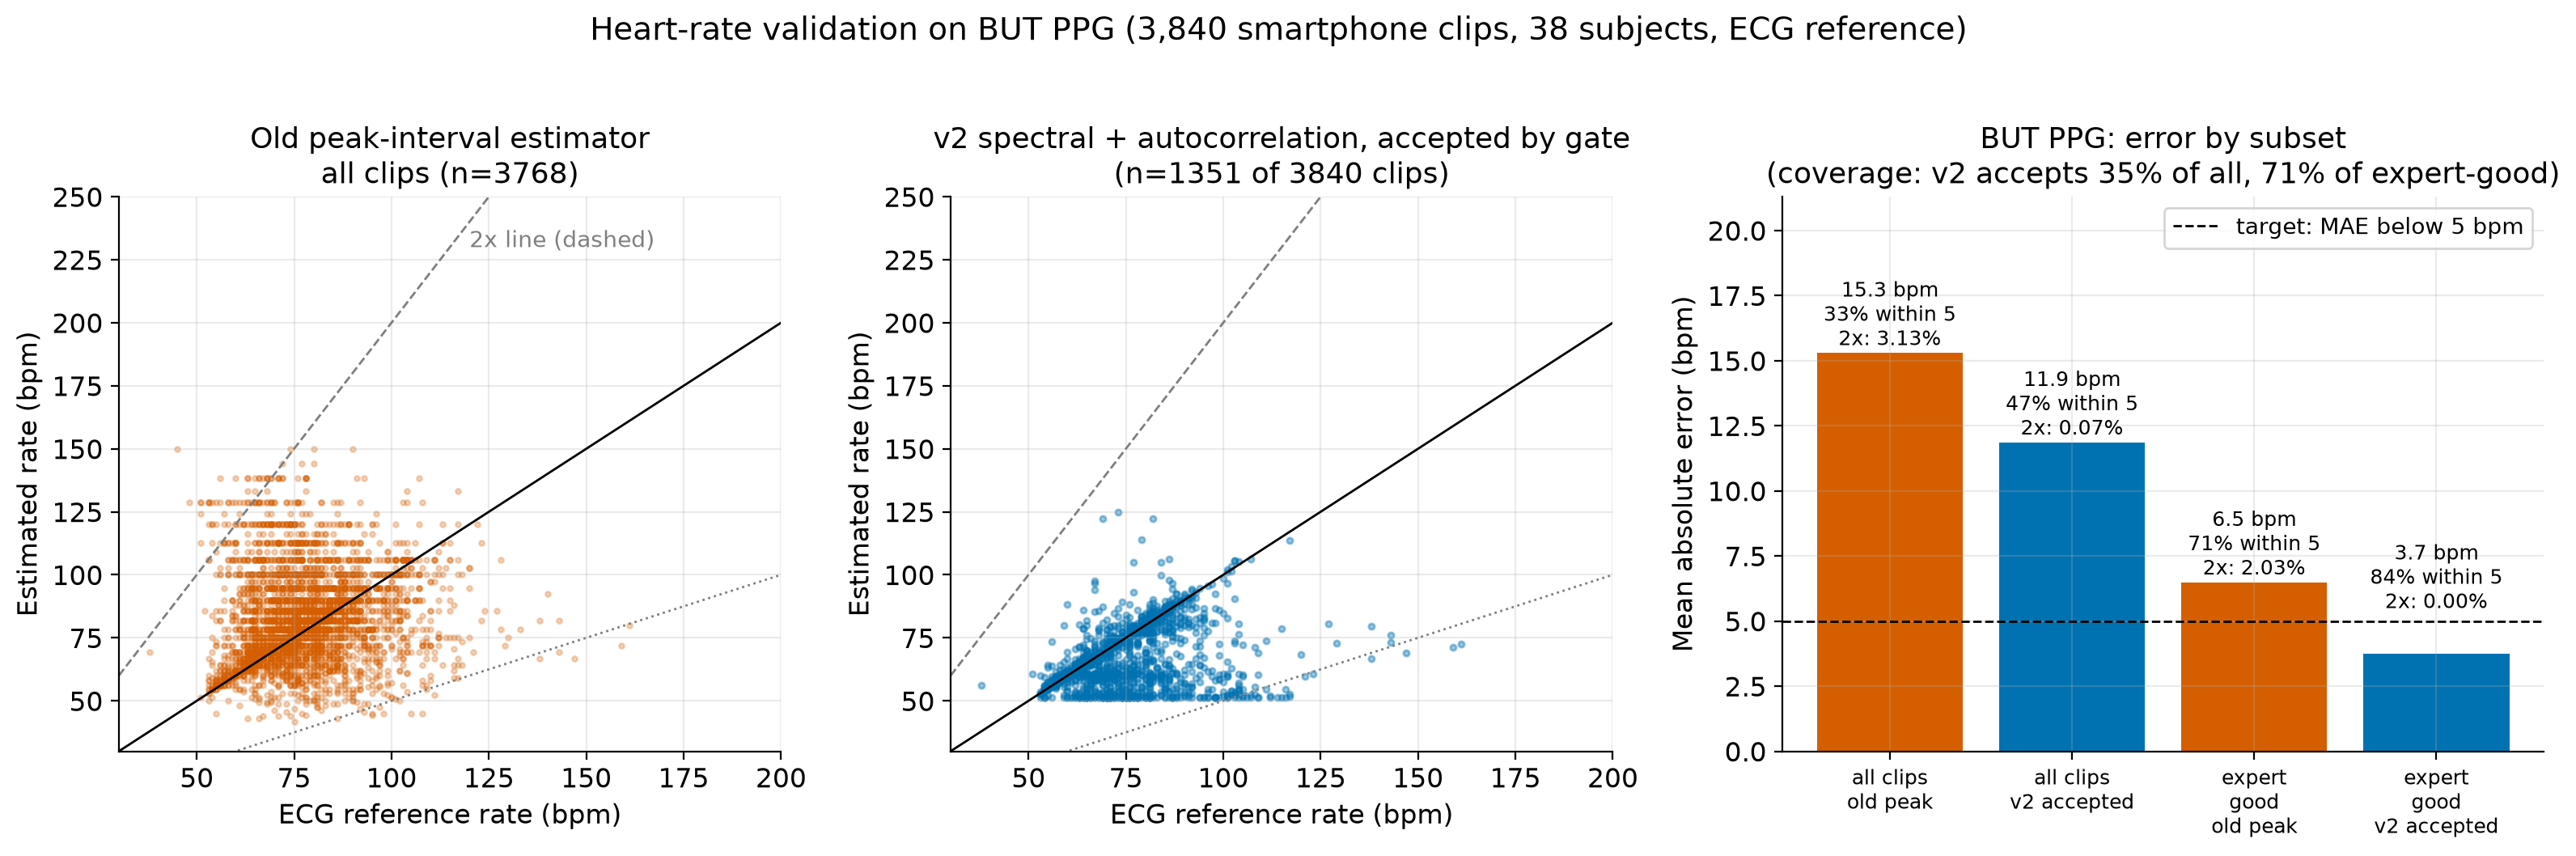
\includegraphics[width=0.84\linewidth]{../docs/figures/fig_hr_validation.png}
\caption{Heart-rate validation on BUT PPG against ECG (\code{results/hr_validation/HR_SUMMARY.csv}). Left: old peak-interval estimator, all clips. Middle: v2 estimator on the 1,351 of 3,840 clips its gate accepts. Right: MAE by subset. The gate trades coverage for accuracy.}\label{fig:hrval}
\end{figure}

\begin{figure}[tbp]
\centering
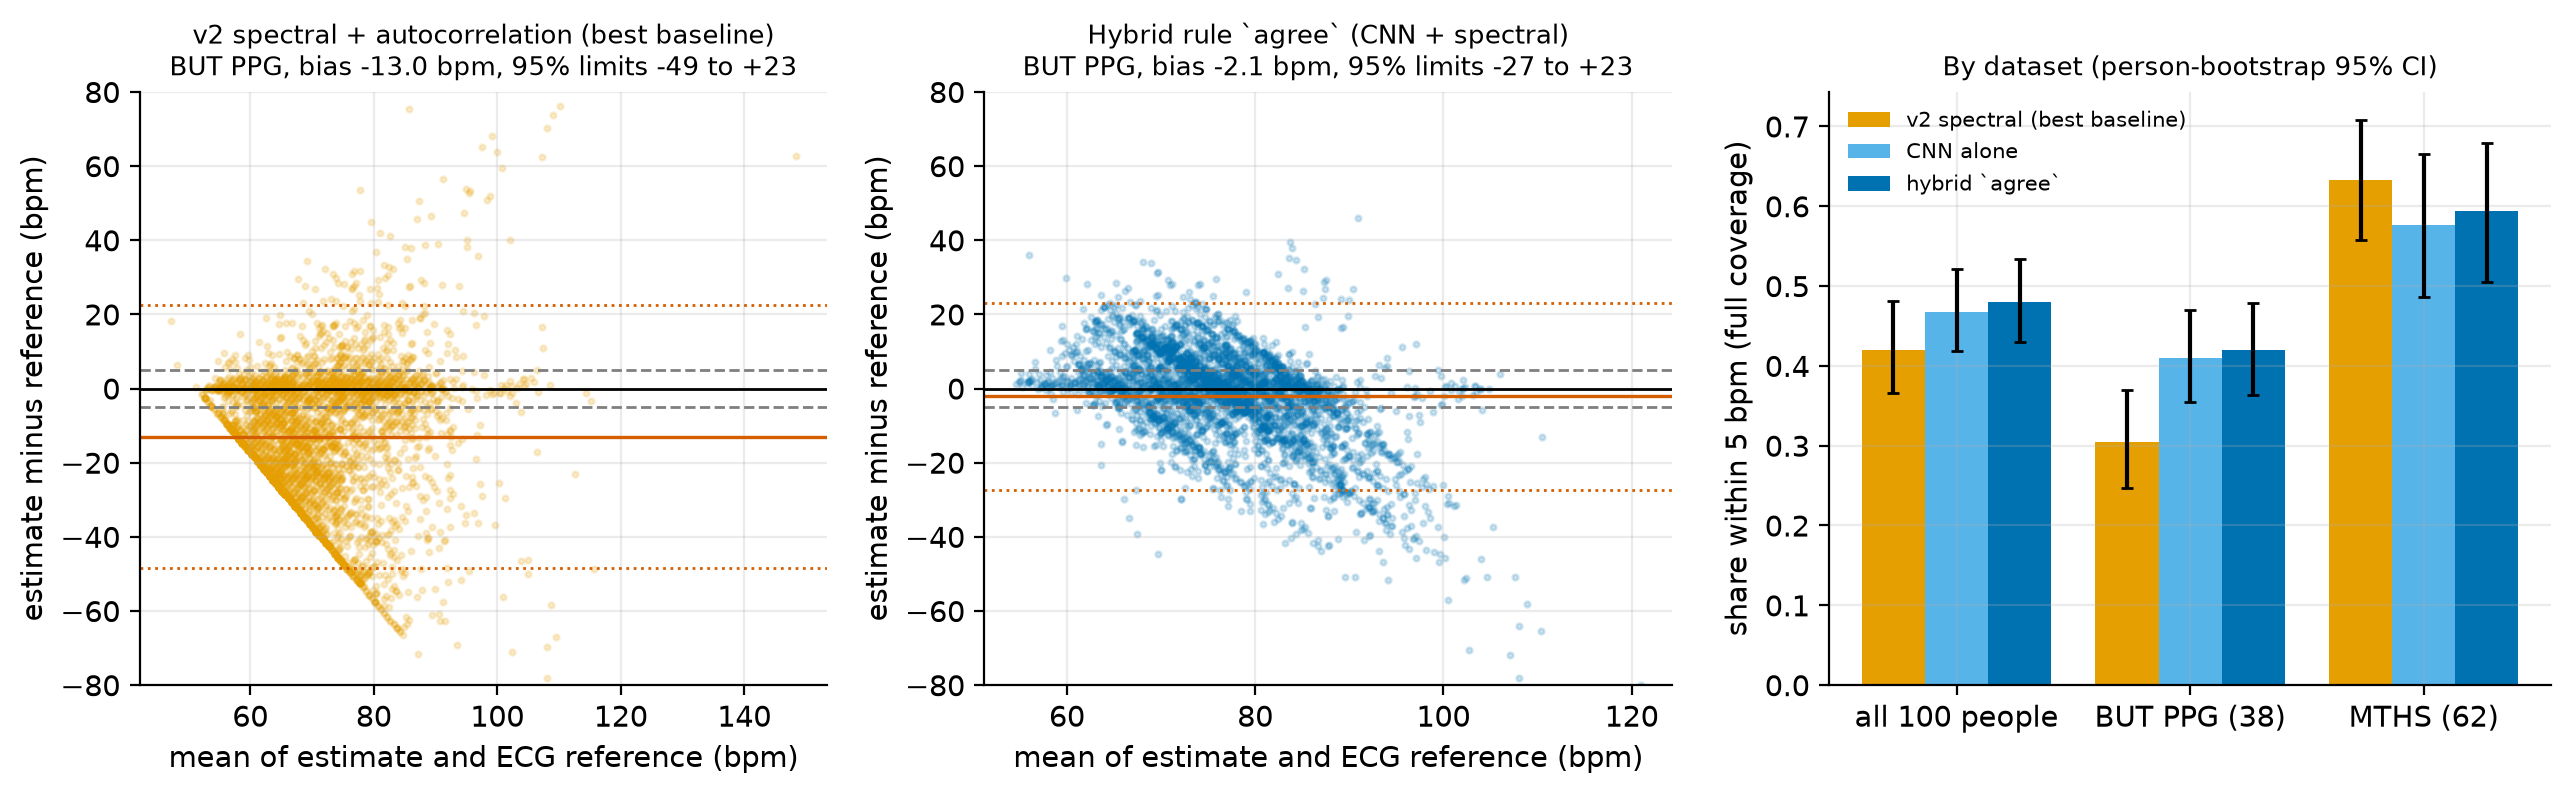
\includegraphics[width=0.84\linewidth]{../docs/figures/ml_hr_blandaltman.png}
\caption{Bland--Altman agreement with ECG on BUT PPG for the v2 spectral estimator (bias $-13.0$~bpm, 95\% limits $-49$ to $+23$; the diagonal edge is the 51~bpm floor) and the post hoc hybrid rule \code{agree} (bias $-2.1$~bpm, limits $-27$ to $+23$); dashed grey lines mark $\pm5$~bpm. Right: share within 5~bpm by dataset with person-bootstrap 95\% intervals.}\label{fig:ba}
\end{figure}

% =====================================================================
\section{Models}\label{sec:models}
Each model outputs per window a score $p$ for \spo{} below 90\%, a forced decision $\hat y=\mathbf{1}[p>0.5]$ and a choice to answer or abstain, shown as \emph{Normal vs your baseline}, \emph{Possible low oxygen: re-check with a pulse oximeter} or \emph{Unsure, re-measure}.

\subsection{Baseline: the logistic chain}\label{sec:chain}
The logistic chain v1 (``the chain'', TINY in some earlier figures) computes 19 features, each made baseline-relative by Eq.~\eqref{eq:base}: heart rate, $\ln$RMSSD and $\ln$SDNN of the inter-beat intervals, two respiratory rates (dominant 0.1 to 0.6~Hz frequency of the beat amplitude and interval series) and beat-amplitude variation; perfusion $\mathrm{pi}_c=\ln\operatorname{sd}(a_c)$; ratios of ratios $\mathrm{ror}_{cd}=\ln[\operatorname{sd}(a_c)/\operatorname{sd}(a_d)]$ for RG, RB and GB, slopes $\operatorname{cov}(a_c,a_d)/\operatorname{var}(a_d)$ for RG and RB, and 30~s versions of the RG slope and ratio; and DC absorbance $\mathrm{dc}_c=\overline{\ell_c}$. Two class-balanced logistic regressions on standardised inputs $z$ are averaged,
\begin{equation}
p_{\mathrm{chain}}=\tfrac12\big[\sigma(\alpha_0+\alpha_1 z_{\mathrm{HR}})+\sigma(\beta_0+\boldsymbol\beta^\top z)\big],\qquad \sigma(u)=1/(1+e^{-u}),
\end{equation}
with inverse regularisation $C=0.01$ and $C=0.1$: 62 numbers in all. A hand-set band answers \emph{Unsure} when $|p-0.5|<0.10$. The heart-rate rise alone reaches AUROC 0.855 on held-out windows. The fixed $C$ came from an earlier search on the same six people; with nested $C$ the chain scores \ChainNestedLzero{} \ChainNestedLzeroCI{} (Table~\ref{tab:clean1}).

\subsection{Colour model}\label{sec:colour}
The colour control is a class-balanced logistic regression ($C=0.1$) on the three baseline-relative log DC values, $p_{\mathrm{dc}}=\sigma(\gamma_0+\sum_{c}\gamma_c\,\widetilde{\mathrm{dc}}_c)$, $c\in\{R,G,B\}$. Deoxyhaemoglobin absorbs more red light than oxyhaemoglobin, so desaturation changes red DC relative to green and blue, while a constant attenuation of every channel cancels in Eq.~\eqref{eq:base}. It shows how much stress robustness needs no network.

\subsection{Self-supervised CNN}\label{sec:cnn}
The earlier engine added to the chain logit the residual of OxyNet, a one-dimensional residual CNN with 167,588 parameters: four stages of two residual blocks (widths 24 to 80, kernel 3, dilations 1 and 2), a 64-dimensional embedding, and a low-oxygen head that reads the window embedding minus the embedding of the person's first minute. Its input is 10 channels of 300 samples ($100\,a_c$ for R, G, B, frame-time delta, two baseline-relative per-beat ratio-of-ratios channels, a beat mask and three baseline-relative log DC channels) and a 9-value side vector. Pretraining is SimCLR contrastive learning \cite{chen2020} on the 299,754-window corpus with the NT-Xent loss
\begin{equation}
\mathcal L_{i,j}=-\ln\frac{\exp(\mathrm{sim}(z_i,z_j)/\tau)}{\sum_{k\ne i}\exp(\mathrm{sim}(z_i,z_k)/\tau)},\qquad\tau=0.2,
\end{equation}
for two augmented views $(i,j)$ of a window, batch 192, Adam at learning rate 0.002 and 2,500 steps, then an OpenOximetry warm-up and fine-tuning inside the folds. The loss falls from 5.28 to 2.10 and the positive view is retrieved 83\% of the time (Fig.~\ref{fig:ssl}); a ridge regression on the frozen embedding predicts Hoffman heart rate at 7.25~bpm MAE against 13.48 for a random encoder.


\begin{figure}[tbp]
\centering
\begin{minipage}[b]{0.56\linewidth}\centering
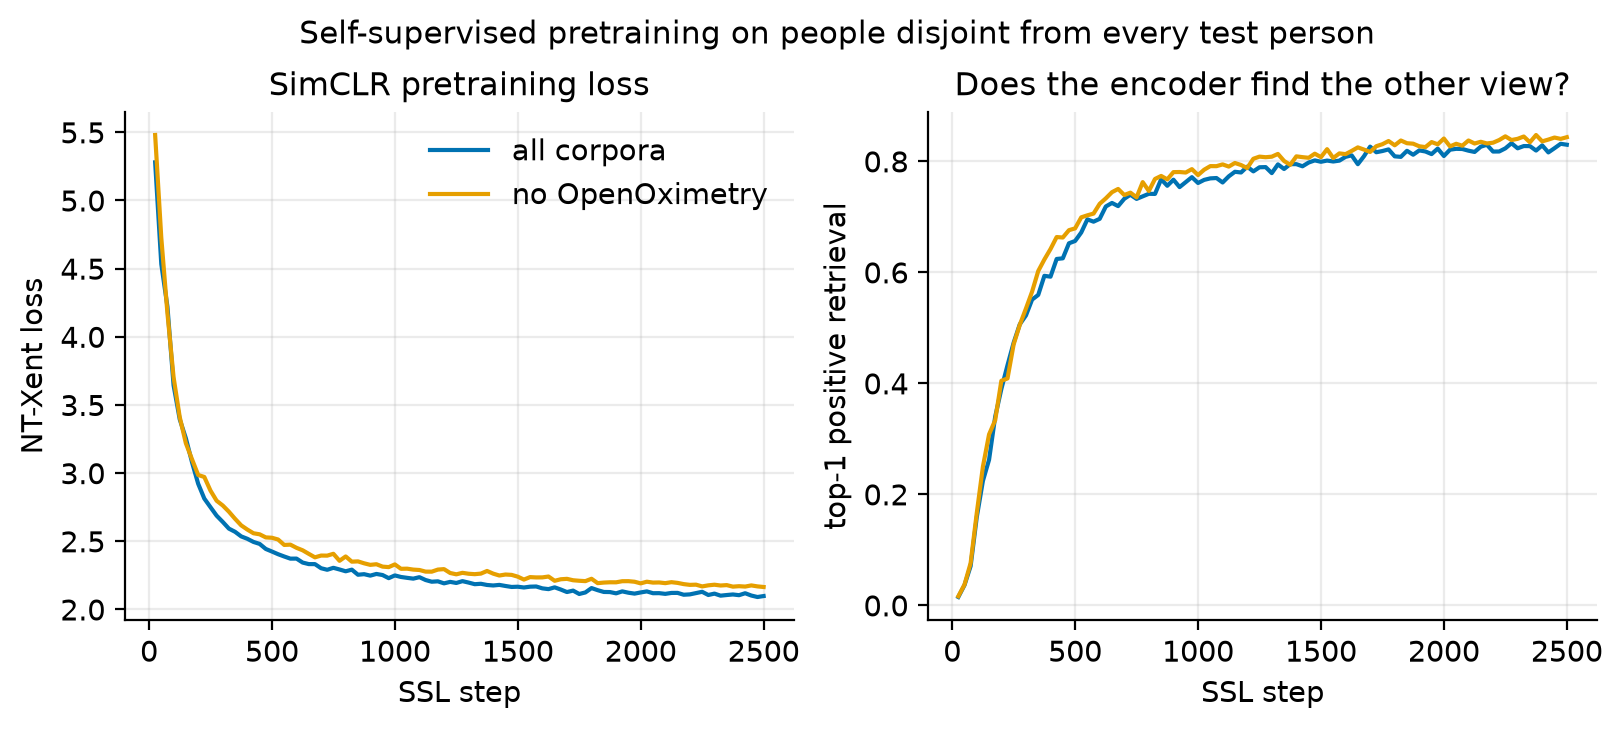
\includegraphics[width=\linewidth]{../docs/figures/ml_ssl_curves.png}
\end{minipage}\hfill
\begin{minipage}[b]{0.41\linewidth}
\caption{Self-supervised pretraining of OxyNet on people disjoint from every test person, with all corpora (299,754 windows) and without OpenOximetry (117,175). Left: NT-Xent loss. Right: top-1 retrieval of the positive view. Both runs learn the contrastive task equally well; the difference appears downstream (Fig.~\ref{fig:ablation}).}\label{fig:ssl}
\end{minipage}
\end{figure}

\subsection{PhotonTwin forward model}\label{sec:twin}
PhotonTwin renders each colour channel from the physical state of a finger: saturation $s$, blood volume fraction $f_b$, melanin fraction $f_m$, pulsatile swing $\alpha$ and source-to-detector separation $\rho$. The absorption is
\begin{equation}
\mu_a(\lambda)=f_b\,\tfrac{2.303\,c_{\mathrm{Hb}}}{64{,}500}\big[s\,\varepsilon_{\mathrm{HbO_2}}(\lambda)+(1-s)\,\varepsilon_{\mathrm{Hb}}(\lambda)\big]+f_m\,\mu_{a,\mathrm{mel}}(\lambda)+\mu_{a,\mathrm{base}}(\lambda),
\end{equation}
with the extinction $\varepsilon$ of Prahl \cite{prahl1998} and $c_{\mathrm{Hb}}=150$~g/l, and from Jacques \cite{jacques1998} ($\lambda$ in nm, cm$^{-1}$)
\begin{equation}
\mu_{a,\mathrm{mel}}=6.6\times10^{11}\lambda^{-3.33},\quad
\mu_s'=2\times10^{5}\lambda^{-1.5}+2\times10^{12}\lambda^{-4},\quad
\mu_{a,\mathrm{base}}=0.244+85.3\,e^{-(\lambda-154)/66.2}.
\end{equation}
Each spectrum is multiplied by a learned scalar, so the physics fixes the shape. The reflectance follows Farrell et al.\ \cite{farrell1992},
\begin{equation}
R(\rho)=\frac{a'}{4\pi}\Big[z_0\Big(\mu_{\mathrm{eff}}+\frac1{r_1}\Big)\frac{e^{-\mu_{\mathrm{eff}}r_1}}{r_1^2}+(z_0+2z_b)\Big(\mu_{\mathrm{eff}}+\frac1{r_2}\Big)\frac{e^{-\mu_{\mathrm{eff}}r_2}}{r_2^2}\Big],
\end{equation}
with $\mu_t'=\mu_a+\mu_s'$, $a'=\mu_s'/\mu_t'$, $z_0=1/\mu_t'$, $z_b=2A/(3\mu_t')$, $\mu_{\mathrm{eff}}=\sqrt{3\mu_a\mu_t'}$, $r_{1}^2=\rho^2+z_0^2$, $r_2^2=\rho^2+(z_0+2z_b)^2$ and $A=(1+R_{\mathrm{eff}})/(1-R_{\mathrm{eff}})$, $R_{\mathrm{eff}}=0.493$ for refractive index 1.4. A channel integrates over the camera sensitivity $S_c$, initialised from the 28-camera database of Jiang et al.\ \cite{jiang2013}, and a white-LED flash spectrum $E$:
\begin{equation}
\ln I_c=\ln\!\int S_c(\lambda)E(\lambda)R(\rho,\lambda)\,d\lambda,\qquad
d_c=\ln I_c\big(f_b(1+\alpha)\big)-\ln I_c(f_b).
\end{equation}
The pulsatile amplitude $d_c$ is a difference of log intensities, the quantity the features measure, so no modified Beer--Lambert step is needed. Sums use log-sum-exp, since blue reflectance underflows at 10~mm. A larger $\rho$ makes the DC fall faster in blue than in red and shifts the light within each band toward longer wavelengths, which moves the ratio-of-ratios calibration.

\subsection{Shipped model: PhotonDistill2}\label{sec:distill}
\paragraph{Features and student} PhotonDistill2 computes 39 causal features: the 19 chain features and 5 respiratory features over a trailing 60~s, both baseline-relative, and 15 absolute signal-quality features (per-channel pulsatile SNR, log perfusion and log DC, clipping, three quantisation measures, autocorrelation and beat fraction). Features are median-imputed, clipped at the training 0.5 and 99.5\% quantiles and standardised with training statistics. A multilayer perceptron
\begin{equation}
\mathbf h=\mathrm{ReLU}\big(W_2\,\mathrm{ReLU}(W_1\mathbf x+\mathbf b_1)+\mathbf b_2\big),\qquad (z,\hat u,a)=W_3\mathbf h+\mathbf b_3,\qquad \mathbf x\in\mathbb R^{39},\ \mathbf h\in\mathbb R^{H},
\end{equation}
outputs a low-oxygen logit $z$, an \spo{} estimate $\hat u\approx(\spo-90)/5$ that is never shown, and an abstain logit $a$ that predicts whether the low-oxygen head is right. Three students with $H=32,32,64$ (2,435, 2,435 and 6,915 parameters) are averaged, $p=\frac13\sum_k\sigma(z_k)$ and $g=\frac13\sum_k\sigma(a_k)$, and the model answers when $g\ge\tau=0.916$. At inference the students run alone in the browser (Fig.~\ref{fig:distill}).

\paragraph{Teachers and dim-flash augmentation} In every outer and inner fold, two teachers are refit on the training people: the chain gives soft targets on clean windows, and the colour model, fit on clean and augmented windows, gives soft targets on augmented copies. A gradient-boosted tree teacher was offered and chosen in 0 of 18 seed folds. Each training recording gets $K=4$ simulated distant-flash copies from the optics prior of Table~\ref{tab:prior}: PhotonTwin rendering, auto-exposure gain, a non-pulsatile leak, shot and read noise, quantisation and occasional loss of green or blue. The copies have their own random stream, asserted disjoint from every evaluation stream, and contain none of the effects of X1. Levels L1 to L5 of Section~\ref{sec:stress} lie inside this prior.

\begin{table}[tbp]
\centering
\caption{Optics prior of the dim-flash augmentation (training people only). $d_\rho$: extra flash-to-lens offset; $\rho_0$: recording separation; path scale: factor on $d_\rho$; $s$, $f_b$, $f_m$, $\alpha$: finger state; leak: fraction of red DC; $k_e$: electrons per digital number (DN).}\label{tab:prior}
{\footnotesize\setlength{\tabcolsep}{4pt}
\begin{adjustbox}{max width=\linewidth}
\begin{tabular}{@{}llllll@{}}
\toprule
Parameter & Prior & Parameter & Prior & Parameter & Prior \\
\midrule
$d_\rho$ (mm) & uniform(0, 12) & $f_m$ & log-uniform(0.01, 0.2) & $k_e$ (e$^-$/DN) & log-uniform($5\times10^4$, $10^6$) \\
$\rho_0$ (mm) & uniform(2.5, 4) & $\alpha$ & log-uniform(0.004, 0.016) & gain cap & log-uniform(128, 2048) \\
path scale & uniform(0.1, 0.3) & leak & uniform(0, 0.4) & exposure error & log-uniform(0.8, 1.25) \\
$s$ & uniform(0.85, 1) & leak tint & log-uniform(0.5, 2) & quantisation (DN) & log-uniform(1/128, 1/4) \\
$f_b$ & log-uniform(0.01, 0.04) & read noise (DN) & log-uniform(0.0005, 0.01) & green / blue lost & Bernoulli(0.15) each \\
\bottomrule
\end{tabular}
\end{adjustbox}}
\end{table}

\paragraph{Loss and nested selection} With label $y$, row weight $\omega$ (class-balanced; 1 clean, 0.25 augmented), teacher logit $t$ and temperature $T$,
\begin{equation}
\mathcal L=\omega\Big[\mathrm{BCE}\big(y,\sigma(z)\big)+\lambda_{\mathrm{kd}}T^2\,\mathrm{BCE}\big(\sigma(t/T),\sigma(z/T)\big)+0.3\,\mathrm{Huber}(\hat u-u)+0.5\,\mathrm{BCE}\big(\mathbf{1}[\hat y=y],\sigma(a)\big)\Big],
\end{equation}
with $u=(\spo-90)/5$, a detached correctness target, and Adam at $3\times10^{-3}$, batch 512. A two-stage grid is scored by leave-one-inner-person-out cross-validation on $0.5\,\mathrm{TM}_{\mathrm{clean}}+0.5\,\overline{\mathrm{TM}}_{\mathrm{aug}}$: teacher set, $\lambda_{\mathrm{kd}}\in\{8,16,32,\text{pure}\}$ and $T\in\{2,4\}$, then $H\in\{16,32,64\}$ and weight decay, with 15 or 30 epochs. Over the 18 seed folds it chose $\lambda_{\mathrm{kd}}=16$ in 7 and 32 in 9 (pure distillation never), and $H=64$ in 7. The threshold $\tau$ is the largest inner out-of-fold coverage at which accuracy $n_{\mathrm{correct}}/(n+1)$ and class-averaged accuracy both reach 0.90 (certified in 17 of 18 folds). Deployed weights are refit on all six people with each seed's modal recipe.

\begin{figure}[tbp]
\centering
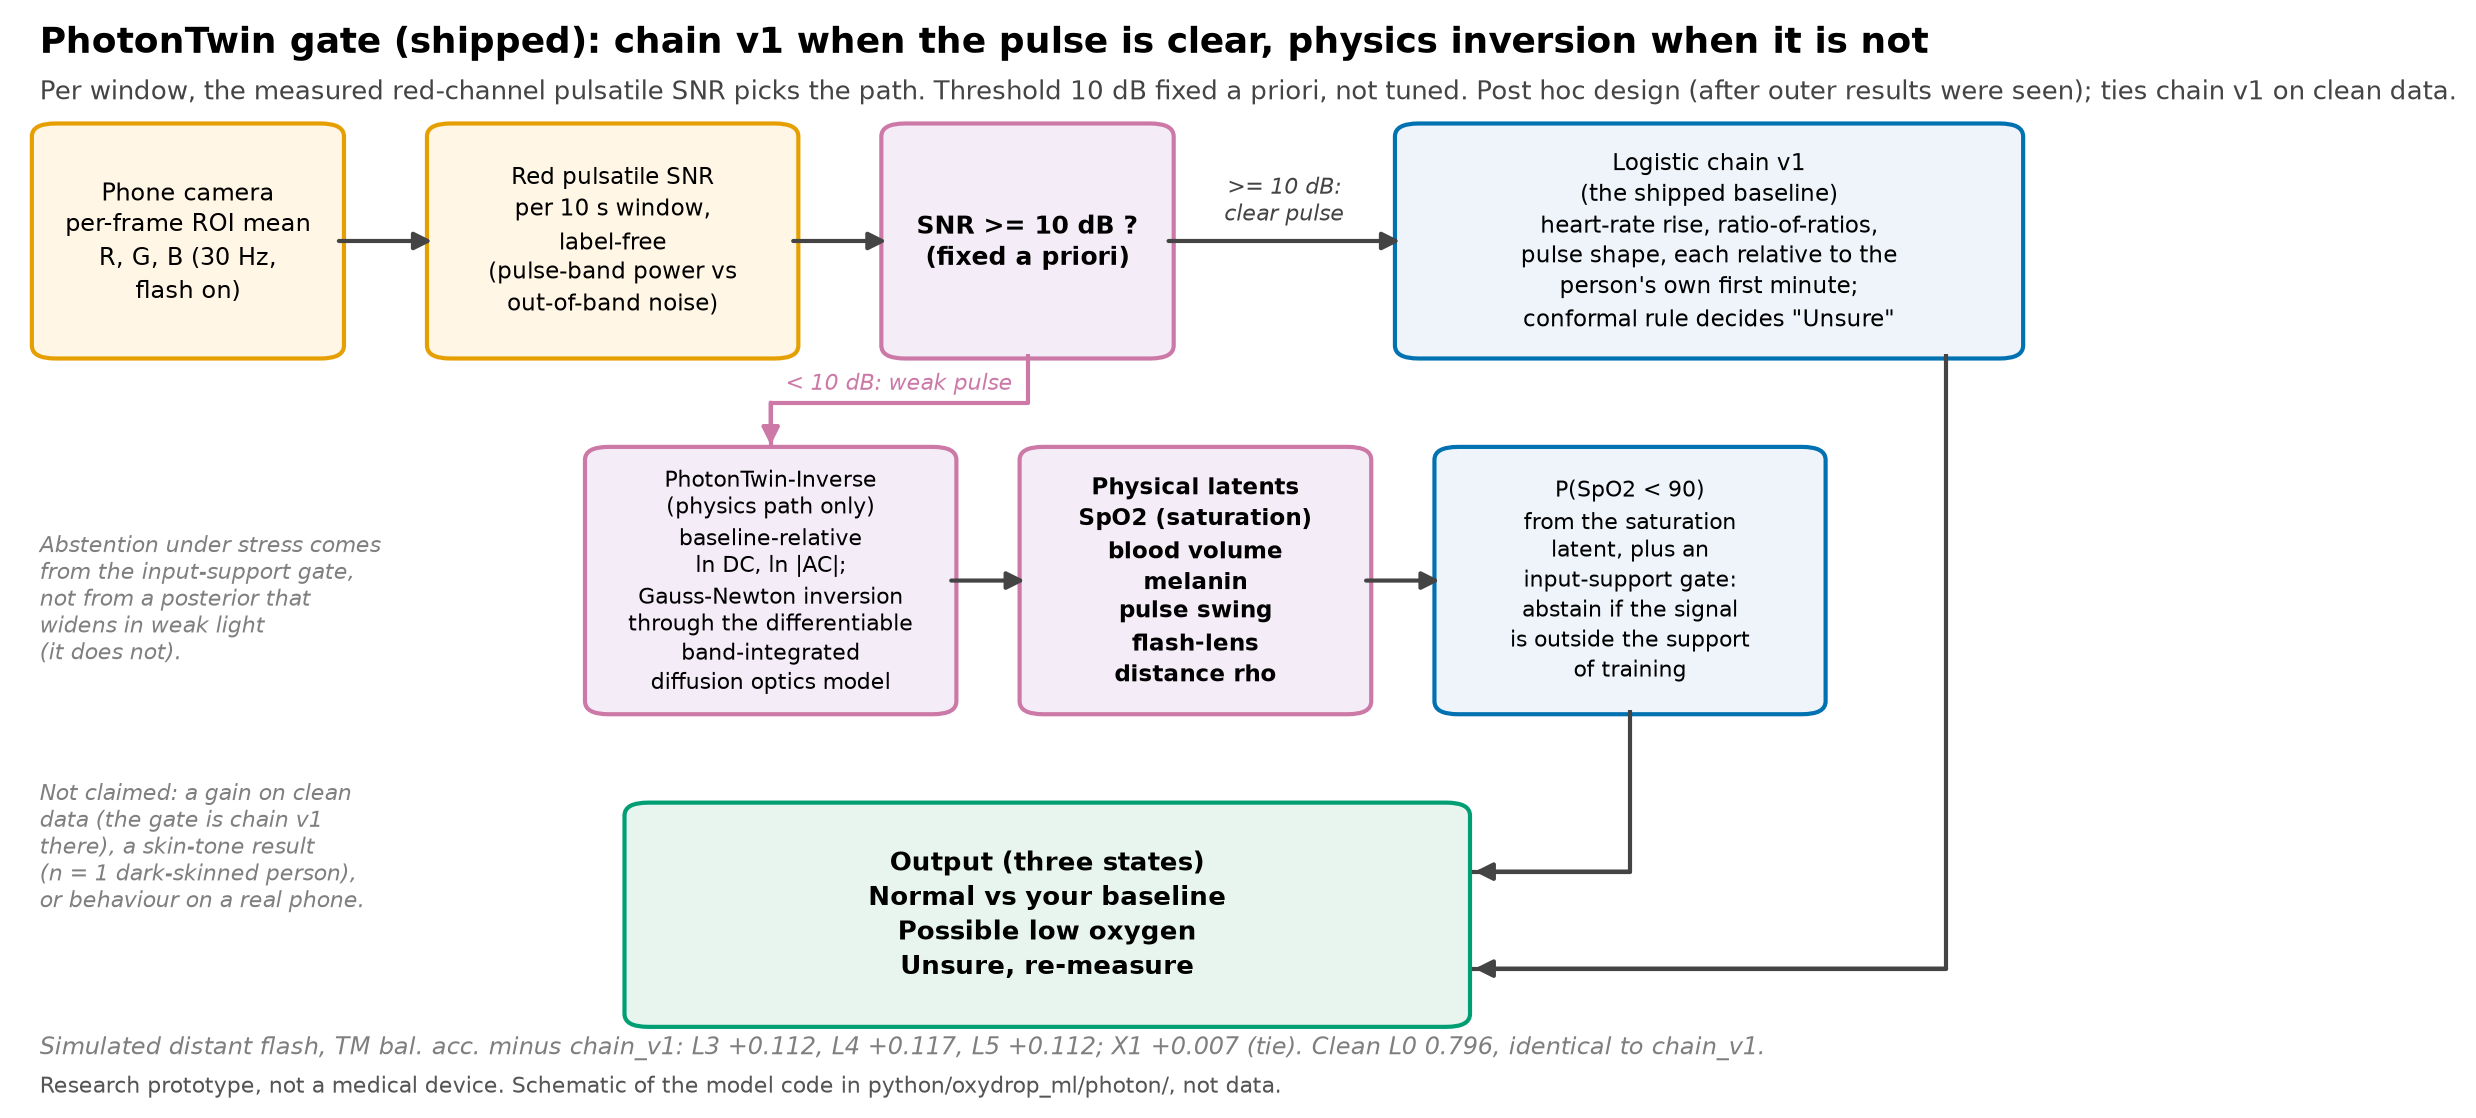
\includegraphics[width=0.9\linewidth]{../docs/figures/photon_architecture.png}
\caption{PhotonDistill2, the shipped model. Top: inference in the browser per 10~s window. Bottom: training only, inside each outer fold on five people; teachers and degraded copies never run at inference. Bottom numbers: LOSO results of Tables~\ref{tab:clean2} and~\ref{tab:stress}.}\label{fig:distill}
\end{figure}

\subsection{Conformal Unsure}\label{sec:conformal}
The earlier hybrid decided \emph{Unsure} by class-conditional split conformal prediction \cite{vovk2012,angelopoulos2023}. With nonconformity $s(w,k)=1-p_k(w)$, $q_k$ is the $\lceil(n_k+1)(1-\alpha)\rceil$-th smallest score of class $k$ among calibration windows of the five other people, and
\begin{equation}
\Gamma_\alpha(w)=\{k: s(w,k)\le q_k\};\qquad \{0\}\mapsto\text{Normal},\quad \{1\}\mapsto\text{Possible low},\quad \{0,1\}\text{ or }\varnothing\mapsto\text{Unsure},
\end{equation}
with $\alpha=0.10$ declared before any score. The shipped student abstains with its learned head instead. For the chain, widening the band $|p-0.5|<c$ raises accuracy on answered windows from 0.870 at full coverage to 0.925 at 85.1\% coverage (\code{results/table_c_coverage.csv}). With the conformal rule (Fig.~\ref{fig:conformal}) the deployed hybrid answers 74.5\% [60.1\%, 84.0\%] of windows at 89.5\% [79.4\%, 98.1\%], while the same step on the chain alone answers 92.5\% at 90.3\%. At the coverage of the chain's band (84.4\%), the hybrid scores 88.0\% against 93.9\%, $-5.9$ [$-17.1$, $+2.3$] points, a tie. Pooled class coverage is near target (91.3\% of hypoxic windows at the 90\% target), but person 1 has 51.3\% of its hypoxic windows called Normal: windows of different people are not exchangeable, and the guarantee fails per person.


\begin{figure}[tbp]
\centering
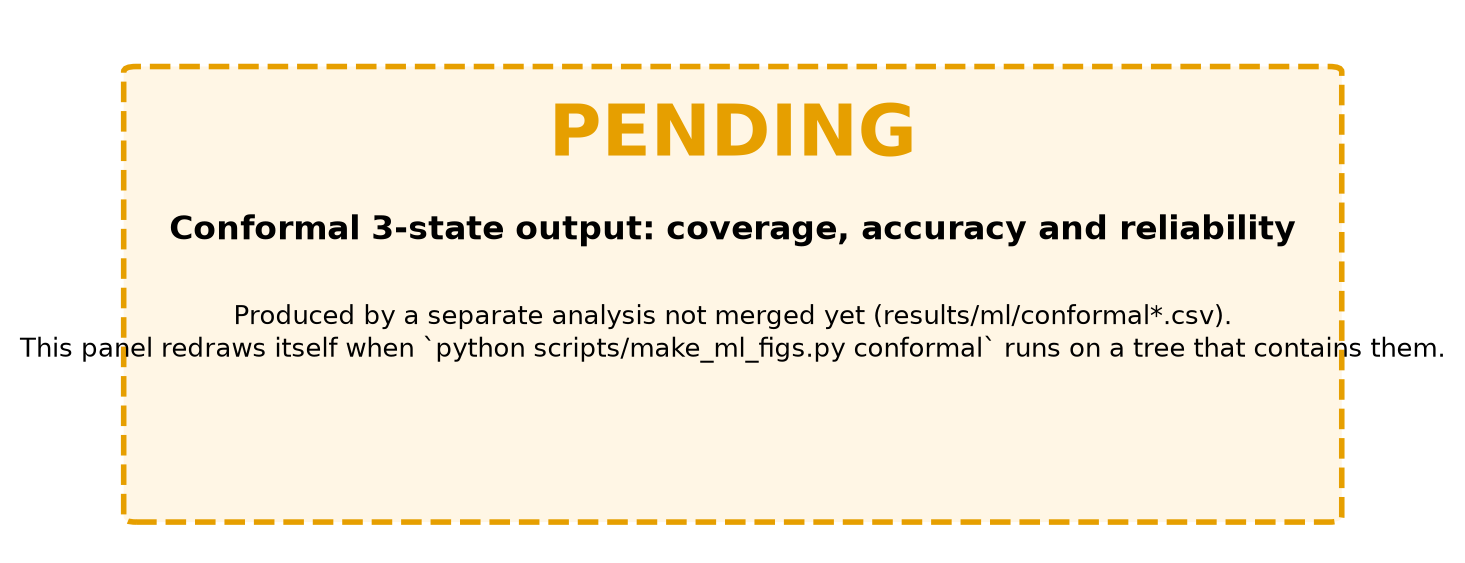
\includegraphics[width=0.74\linewidth]{../docs/figures/ml_conformal.png}
\caption{Conformal three-state output on Hoffman with thresholds from the other five people (\code{results/ml/conformal_*.csv}). Left: accuracy on answered windows against coverage as $\alpha$ varies, with person-bootstrap bands; dots mark $\alpha=0.10$, the star and cross the hand-set v1 and v2 bands. The chain alone dominates both hybrids. Right: hypoxic windows called Normal per person at $\alpha=0.10$; person 1 is far above the 10\% target.}\label{fig:conformal}
\end{figure}

% =====================================================================
\section{Evaluation Protocol}\label{sec:protocol}
\paragraph{Leave-one-person-out with nested folds} Each outer fold holds out one person with both hands, which share the reference at matched times; there is no window-level split. Hyperparameters, epochs, thresholds, distillation weights, teachers and ensemble members are chosen by person-grouped cross-validation on the five training people. Scalers, imputation values, teachers and conformal thresholds are fitted on training people only, and the held-out labels are read only to score. The headline is the three-seed ensemble. The pre-registration predates every learned-model result, and numbered amendments state what had been seen at each change.

\paragraph{No test leakage} Augmented copies come from training recordings only, pretraining uses only people who are never test people, and saved out-of-fold scores of other candidates were not used as teachers, because each came from a model trained on another fold's held-out person.

\paragraph{Time-matched balanced accuracy} \spo{} falls over time in a staircase protocol, so a clock-only predictor reaches 83.5\% plain accuracy and AUROC 0.819 here (\code{results/table_a_main.csv}). Windows are therefore grouped into 100~s bins of elapsed time, and a bin counts only if both classes have at least five windows and 8\% of the bin. With $m_k$ the smaller class count in bin $k$, and $\mathrm{tpr}_k$, $\mathrm{tnr}_k$ the sensitivity and specificity of the forced decision there,
\begin{equation}
\mathrm{TM}=\frac{\sum_k m_k(\mathrm{tpr}_k+\mathrm{tnr}_k)/2}{\sum_k m_k}.
\end{equation}
A clock-only predictor and the majority class both score 0.50. Abstention is scored separately.

\paragraph{Person bootstrap and paired differences} Intervals resample the six people $B=2{,}000$ times, with the same resamples for every model. For resample $b$ with people $\mathcal P^{(b)}$, $\Delta^{(b)}=\mathrm{TM}_{\mathrm{model}}(\mathcal P^{(b)})-\mathrm{TM}_{\mathrm{chain}}(\mathcal P^{(b)})$, and the 2.5th and 97.5th percentiles form the 95\% interval \cite{efron1979}. Six people allow only 462 distinct resamples, so the intervals are coarse. We also count the people whose own TM beats the chain's, with a one-sided sign test (6/6: $p=0.016$; 5/6: $p=0.109$; 4/6: $p=0.344$). A model \emph{beats} the chain only if the paired interval lies above 0, at least 5 of 6 people improve, its worst person is not below the chain's and its null control passes. An interval containing 0 is a \emph{tie}; one below 0 is a \emph{loss}.

\paragraph{Null controls and design rounds} Each full pipeline, inner search and teachers included, is retrained on labels permuted across training windows \cite{ojala2010}, usually with three draws; a mean TM above 0.55 fails. The chain refit on \ChainNullN{} permutations has mean \ChainNullMean{} (SD \ChainNullSD{}, range \ChainNullMin{} to \ChainNullMax{}), so the rule uses the mean. Round~1 was designed before any score on this harness, round~2 after round~1's outer results and round~3 after round~2's, each with a rule fixed before its first score. Round~3 replaced the round-2 winner only with a higher clean-light estimate, a paired difference to it with lower bound above $-0.02$, a mean paired stress gain over L3 to X1 of at least 0, and passed nulls.

% =====================================================================
\section{Results}\label{sec:results}
Numbers are from \code{results/photon/TABLE.csv} unless another file is named; intervals are 95\% person-bootstrap intervals.

\subsection{Clean light}
PhotonDistill2 scores \WinLzero{} \WinLzeroCI{} against \ChainLzero{} \ChainLzeroCI{} for the chain (Fig.~\ref{fig:barrel}a), a paired difference of \WinLzeroDiff{} \WinLzeroDiffCI{} with \WinLzeroBetter{} people better. By the rule above this is a tie: the model is on par with the chain and does not beat it. Its worst person scores \WinLzeroWorst{} against \ChainLzeroWorst{}, and its AUROC is \WinLzeroAuroc{} against \ChainLzeroAuroc{}. Tables~\ref{tab:clean1} and~\ref{tab:clean2} list every candidate. No model beats the chain on clean light. Against the round-2 model it replaced, PhotonDistill2 differs by \WinVsDistillLzero{} \WinVsDistillLzeroCI{}. Its null draws score \WinNullList{} (mean \WinNullMean{}); the post hoc PhotonTwin gate (null mean 0.584), PhotonNet (0.618) and OxySSL (0.643) fail the null rule.

The locked run trained on a CPU. A rerun of the same code on a Kaggle T4 GPU scored \DistillTwoGpuLzero{} \DistillTwoGpuLzeroCI{}, paired to the chain \DistillTwoGpuLzeroDiff{} \DistillTwoGpuLzeroDiffCI{}: a different float32 summation order changed which grid point won the inner search in 5 of 18 seed folds. We report the gap as seed and hardware variance. The rerun's interval lies just below 0, neither run beats the chain, and the app ships the locked run.

\begin{table}[tbp]
\centering
\caption{Clean light (L0), part 1: baselines, controls without a network, and round~1 (designed before any score on this harness). TM: time-matched balanced accuracy of the forced decision. $\Delta$: model minus chain on the same resampled people. Better: people whose own TM beats the chain's. Worst: TM of the worst person. Hybrid and CNN are converted from the earlier pipeline at L0 only.}\label{tab:clean1}
{\footnotesize\setlength{\tabcolsep}{4pt}
\begin{tabular}{@{}p{5.0cm}llcccc@{}}
\toprule
Model & TM [95\% CI] & $\Delta$ vs chain [95\% CI] & Verdict & Better & Worst & AUROC \\
\midrule
\multicolumn{7}{@{}l}{\emph{Baselines}} \\
Logistic chain v1 (reference) & \ChainLzero{} \ChainLzeroCI & reference & & & \ChainLzeroWorst & \ChainLzeroAuroc \\
\cleanrow{Logistic chain v1, $C$ by nested CV}{ChainNested}
\cleanrow{Hybrid (chain + CNN), nested}{Hybrid}
\cleanrow{CNN alone (OxyNet, 3 seeds)}{Cnn}
\multicolumn{7}{@{}l}{\emph{Controls (no network)}} \\
\cleanrow{DC-colour LR (3 values)}{DcLr}
\cleanrow{DC colour + AC optics LR}{DcRorLr}
\cleanrow{DC colour + $\Delta$HR LR}{DcHrLr}
\multicolumn{7}{@{}l}{\emph{Round 1}} \\
\cleanrow{PhotonTwin-Inverse}{TwinInv}
\cleanrow{PhotonTwin-Inverse, physics path only}{TwinInvNoResid}
\cleanrow{FlashGap}{Flashgap}
\cleanrow{OxyTrack (outer folds seen in development)}{Oxytrack}
\cleanrow{PhotonTwin gate (hand-coded, post hoc)}{TwinGate}
\cleanrow{FlashGap gate (post hoc)}{FlashgapGate}
\bottomrule
\end{tabular}}
\end{table}

\begin{table}[tbp]
\centering
\caption{Clean light (L0), part 2: rounds 2 and 3, designed after earlier held-out results had been seen. Columns as in Table~\ref{tab:clean1}. PhotonNet and OxySSL fail their null controls. Ens-3, a stack of three models, landed after the round-3 lock without null controls and was not eligible.}\label{tab:clean2}
{\footnotesize\setlength{\tabcolsep}{4pt}
\begin{tabular}{@{}p{5.0cm}llcccc@{}}
\toprule
Model & TM [95\% CI] & $\Delta$ vs chain [95\% CI] & Verdict & Better & Worst & AUROC \\
\midrule
\multicolumn{7}{@{}l}{\emph{Round 2 (trained end to end)}} \\
\cleanrow{PhotonDistill (round-2 winner, replaced)}{Distill}
\cleanrow{OxySeq}{Oxyseq}
\cleanrow{PhotonNet}{Photonnet}
\cleanrow{OxySSL}{Oxyssl}
\multicolumn{7}{@{}l}{\emph{Round 3 (scaled up)}} \\
\cleanrow{\textbf{PhotonDistill2 (shipped)}}{Win}
\cleanrow{PhotonDistill2, GPU rerun (seed variance)}{DistillTwoGpu}
\cleanrow{MultiDA}{Multida}
\cleanrow{PhotonNet-XL}{PhotonnetXl}
\cleanrow{Ens-3 (not eligible)}{EnsThree}
\bottomrule
\end{tabular}}
\end{table}



\paragraph{Reliability and confusion} On clean light the shipped model answers 3,896 of 5,644 windows (coverage \WinLzeroCov{}) and is right on 93.3\% of them; its all-window balanced accuracy is 0.866, so abstention removes the harder windows. The forced decision classifies 86.6\% of normal windows (2,079 of 2,400) and 86.6\% of low windows (2,809 of 3,244) correctly (Fig.~\ref{fig:barrel}b). The \spo{} head has an MAE of \WinLzeroMae{} points and is never shown.

\begin{figure}[tbp]
\centering
\begin{minipage}[b]{0.41\linewidth}\centering
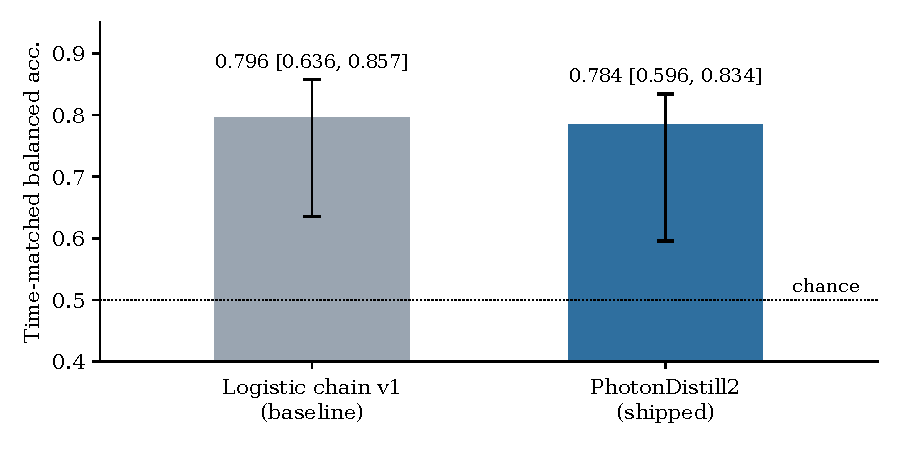
\includegraphics[width=\linewidth]{figures_ieee/fig_bar.pdf}\\{\small (a)}
\end{minipage}\hfill
\begin{minipage}[b]{0.57\linewidth}\centering
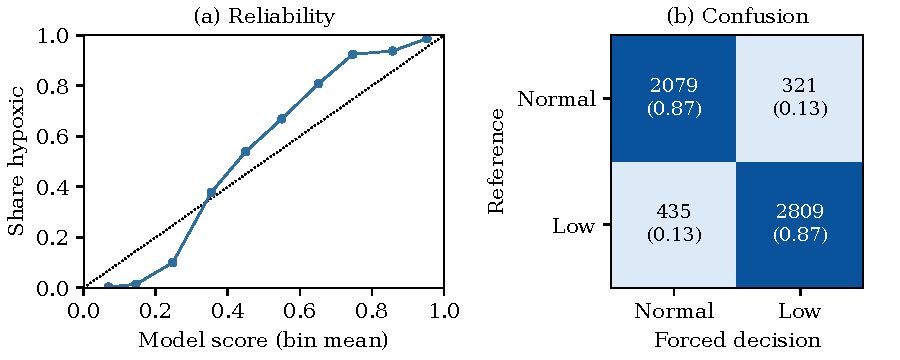
\includegraphics[width=\linewidth]{figures_ieee/fig_reliability.pdf}\\{\small (b)}
\end{minipage}
\caption{(a) Clean-light TM of the chain and PhotonDistill2 with 95\% person-bootstrap intervals; paired difference \WinLzeroDiff{} \WinLzeroDiffCI{}, a tie. (b) Pooled held-out predictions of PhotonDistill2 (5,644 windows): share of low windows per score bin (bins with at least 20 windows) and the confusion matrix of the forced decision with row fractions.}\label{fig:barrel}
\end{figure}

\paragraph{ROC and the train-versus-test gap} In an earlier scoring run of the same protocol (Fig.~\ref{fig:roc}) the chain has AUROC 0.942, the heart-rate rise alone 0.855 and the time-only clock 0.819. Comparing each model's score on its own training people with its held-out score (\code{results/ml/}), gradient-boosted trees on 26 hand-crafted features lose 0.170 and the chain 0.041.

\begin{figure}[tbp]
\centering
\begin{minipage}[b]{0.36\linewidth}\centering
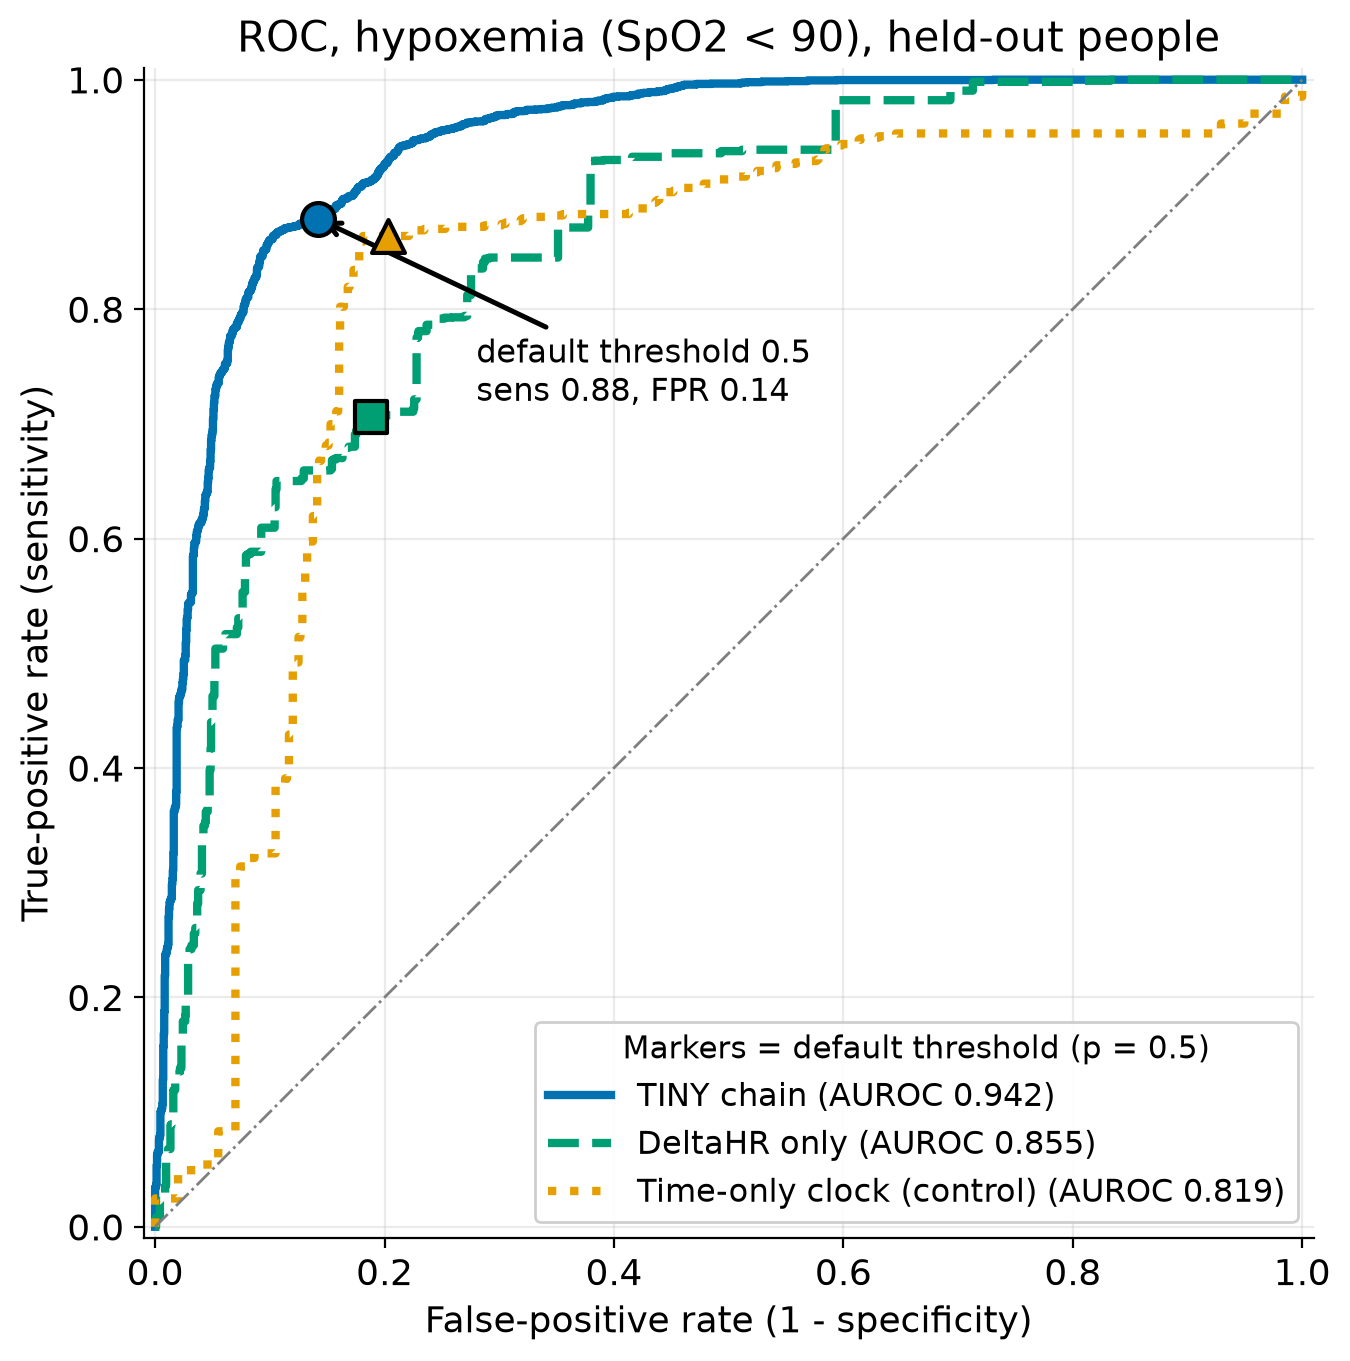
\includegraphics[width=\linewidth]{../docs/figures/fig_roc.png}
\end{minipage}\hfill
\begin{minipage}[b]{0.6\linewidth}
\caption{ROC of the chain (``TINY''), the heart-rate rise alone and the time-only clock on pooled held-out windows of an earlier scoring run (\code{results/table_a_main.csv}); markers are the 0.5 threshold. The clock's AUROC comes from the staircase, not from oxygen, which is why the headlines use TM.}\label{fig:roc}
\end{minipage}
\end{figure}

\paragraph{Per person} Per-person TM for persons 1 to 6 is 0.889, 0.458, 0.660, 0.711, 0.737 and 0.539 for the chain and 0.673, 0.500, 0.666, 0.714, 0.718 and 0.551 for PhotonDistill2 (\code{paper/tables/tab_person.tex}); the colour control is best on person 6 (0.869). The chain, the CNN and the hybrids show the same complementary errors, and no combiner learned from five people exploits them (Fig.~\ref{fig:pp}). In plain accuracy at the default threshold the chain's worst person is person 4 at 0.775 (\code{results/table_b_per_person.csv}), while the time-only clock reaches 0.54 to 0.96 per person from elapsed time alone. Person 4's slow resting pulse lies below the v2 heart-rate band.


\begin{figure}[tbp]
\centering
\begin{minipage}[b]{0.5\linewidth}\centering
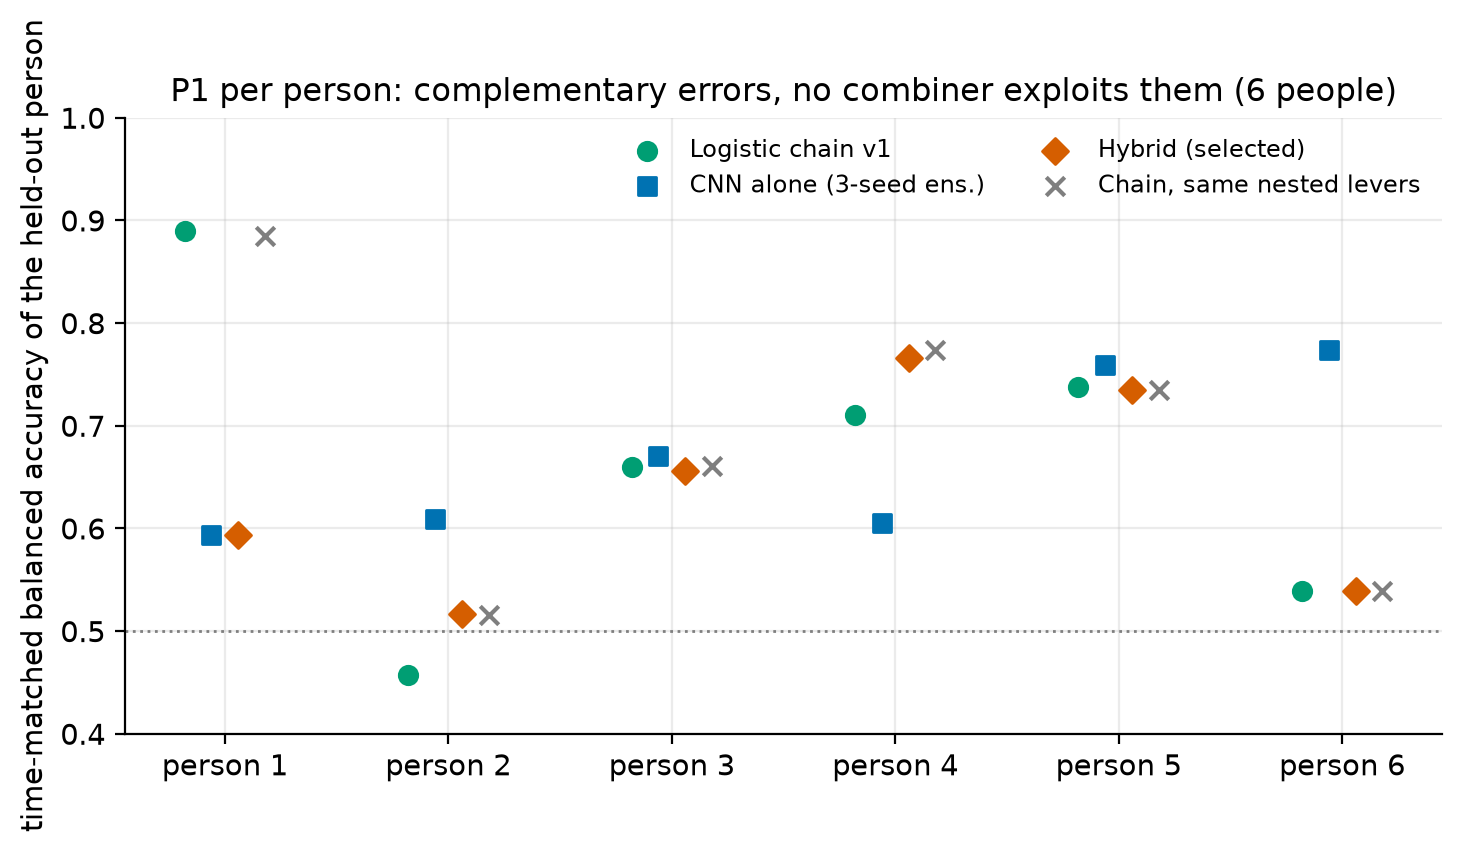
\includegraphics[width=\linewidth]{../docs/figures/ml_p1_per_person.png}
\end{minipage}\hfill
\begin{minipage}[b]{0.47\linewidth}
\caption{Clean-light TM of each held-out person for the chain, the CNN alone (three-seed ensemble), the per-person-selected hybrid and a chain refit with the same nested levers (\code{results/ml/}). The chain wins on person 1 and the CNN on person 6, but no combination chosen on five people captures both.}\label{fig:pp}
\end{minipage}
\end{figure}


\paragraph{Chain v1 against v2} The v2 chain replaced the beat counter with the gated estimator of Section~\ref{sec:hr} and required a pulse lock. On Hoffman this did not help (Fig.~\ref{fig:v1v2}, \code{results/eval_v1_vs_v2.csv}). Forced to answer every window, v2 scores 80.5\% accuracy against 87.5\% for v1, with worst person 0.49 against 0.81, and TM 0.771 against 0.796. With the abstention band, v1 answers 84.4\% of windows at 93.9\% and v2 68.0\% at 94.7\%. Person 4 rests at 43~bpm, below the 51~bpm floor, so v2 never locks on that person.

\begin{figure}[tbp]
\centering
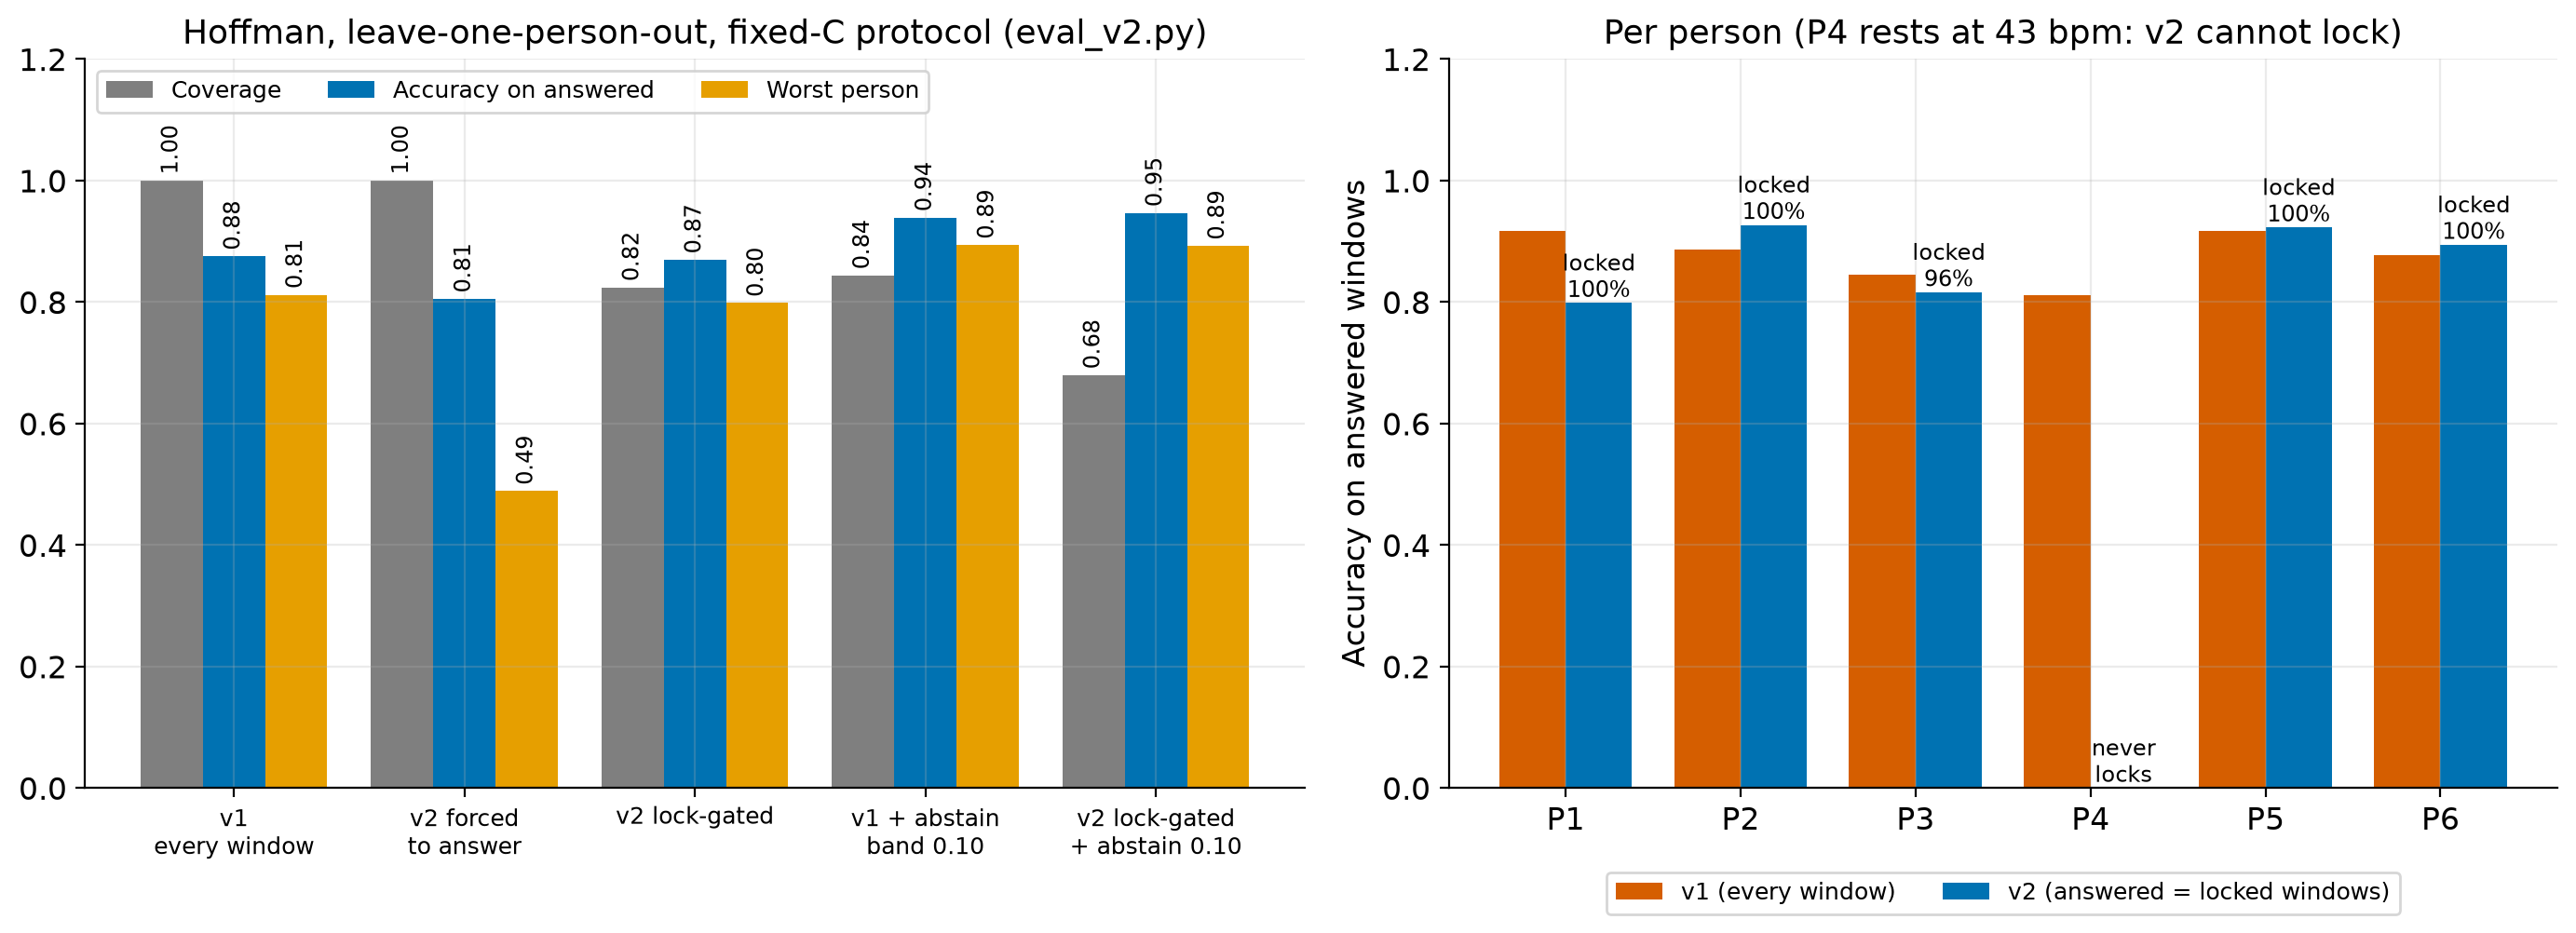
\includegraphics[width=0.7\linewidth]{../docs/figures/fig_v1_vs_v2.png}
\caption{Chain v1 (beat-counting heart rate) against v2 (gated spectral heart rate) on Hoffman, LOSO with fixed $C$ (\code{results/eval_v1_vs_v2.csv}). Left: coverage, accuracy on answered windows and worst person for five operating modes. Right: accuracy per person; v2 answers only windows with a pulse lock and never locks on person 4.}\label{fig:v1v2}
\end{figure}

\paragraph{Ablations} Removing the teachers from PhotonDistill drops clean-light TM from \DistillLzero{} to \DistillNoKdLzero{}, so distillation adds about 0.10; the first grid, before the post hoc widening, scored \DistillVoneLzero{}. OxySeq without test-time adaptation scores \OxyseqNoTtaLzero{} (against \OxyseqLzero{}), PhotonNet without its physics layer \PhotonnetNoPhysLzero{} (against \PhotonnetLzero{}), OxySSL with its pretraining used only as initialisation \OxysslInitLzero{} and without augmentation \OxysslNoAugLzero{} (against \OxysslLzero{}), and MultiDA on Hoffman rows only \MultidaHofonlyLzero{} (against \MultidaLzero{}). For OxyNet (Fig.~\ref{fig:ablation}), the OpenOximetry warm-up is the main source of skill: the full CNN scores 0.739 [0.574, 0.811], without OpenOximetry 0.577 and without any pretraining 0.550. Removing self-supervision, physics channels, augmentation or baseline conditioning moves TM by about the seed spread of 0.019, although removing baseline conditioning widens the train-versus-test gap from $-0.015$ to $+0.105$. Test-time BatchNorm adaptation hurt (0.638 against 0.752 for seed 0).


\begin{figure}[tbp]
\centering
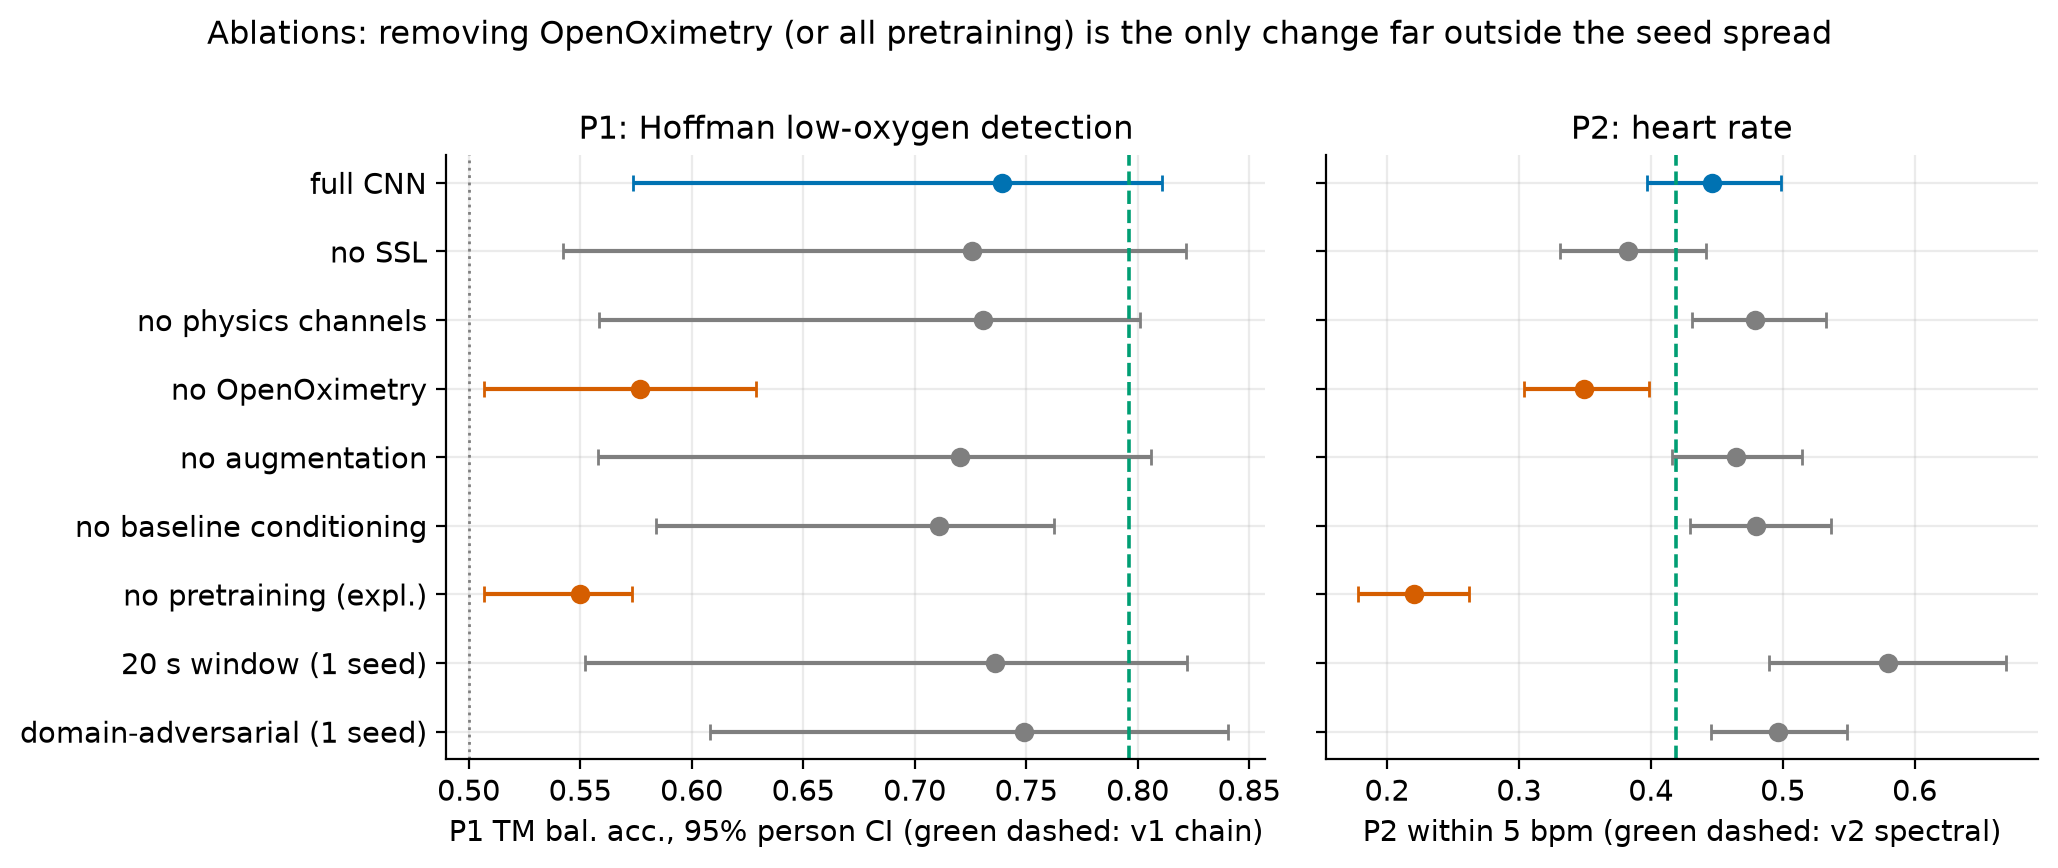
\includegraphics[width=0.7\linewidth]{../docs/figures/ml_ablation.png}
\caption{Ablations of OxyNet with 95\% person-bootstrap intervals (\code{results/ml/ablation_core.csv}). Left: low-oxygen TM on Hoffman (dashed: chain). Right: heart rate within 5~bpm (dashed: v2 spectral). Removing OpenOximetry or all pretraining is the only change far outside the seed spread. ``1 seed'' rows use a grouped protocol.}\label{fig:ablation}
\end{figure}

% =====================================================================
\section{Stress Test (Simulation)}\label{sec:stress}
\subsection{Design}
The stress test simulates a phone whose flash sits farther from the lens than on the recording phone; it measures no phone. Only the held-out recording is degraded, and models are not refit per level. On the per-frame ROI means the simulator (i)~splits each channel into DC (centred 5~s moving average) and pulsatile part; (ii)~renders a nominal finger ($s=0.97$, $f_b=0.02$, $f_m=0.03$) with PhotonTwin at $\rho_0=3$~mm and at $\rho_0+0.25\,d_\rho$, giving a DC attenuation $a_c$ and pulsatile gain $m_c$ per channel; (iii)~applies an auto-exposure gain $g=\min(1/a_R,1024)$; (iv)~adds a non-pulsatile leak, a fraction of the red light; (v)~adds shot noise $\sqrt{g(\text{signal}+\text{leak})/K}$ with $K=2\times10^5$ electrons per DN and read noise $0.002\,g$~DN; and (vi)~quantises to 1/32~DN. The path factor 0.25 was fixed from the input-side SNR before any model was scored on a degraded recording, since a semi-infinite medium over-attenuates a finger. Table~\ref{tab:stressdef} lists the levels; the median red-channel pulse SNR is \StressSNR{}~dB at levels 1 to 5. X1 uses the L3 optics and leak, then adds motion-like DC steps, AR(1) correlated noise ($\phi=0.7$), sample-and-hold frame drops and a per-channel tone curve (gamma 0.75, 0.80, 0.85). None of these is in the augmentation prior, so X1 is the only out-of-family level.

\begin{table}[tbp]
\centering
\caption{Simulated distant-flash levels (\code{results/photon/HARNESS.md}): added offset $d_\rho$, share of DC light kept per channel, pulsatile gain $m_c$, auto-exposure gain, leak fraction and read noise after gain. Blue dies first, red last.}\label{tab:stressdef}
\begin{adjustbox}{max width=\linewidth}% GENERATED from results/photon/HARNESS.md
{\footnotesize\setlength{\tabcolsep}{4pt}
\begin{tabular}{rrrrrrrrr}
\toprule
Level & $d_\rho$ (mm) & Red kept & Green kept & Blue kept & $m_c$ R / G / B & Gain & Leak & Read noise (DN) \\
\midrule
0 & 0 & 1 & 1 & 1 & 1.00 / 1.00 / 1.00 & 1 & 0 \% & 0.002 \\
1 & 2 & 0.171 & 0.14 & 0.103 & 1.01 / 1.00 / 0.77 & 6 & 2 \% & 0.0117 \\
2 & 4 & 0.0309 & 0.0207 & 0.012 & 1.03 / 1.00 / 0.74 & 32 & 5 \% & 0.0646 \\
3 & 6 & 0.00586 & 0.00322 & 0.00147 & 1.04 / 0.99 / 0.74 & 171 & 10 \% & 0.341 \\
4 & 8 & 0.00116 & 0.000522 & 0.000188 & 1.05 / 0.98 / 0.74 & 862 & 20 \% & 1.72 \\
5 & 10 & 0.000238 & $8.8\times10^{-5}$ & $2.49\times10^{-5}$ & 1.07 / 0.96 / 0.74 & 1024 (cap) & 35 \% & 2.05 \\
\bottomrule
\end{tabular}}
\end{adjustbox}
\end{table}

\subsection{Results}
The chain falls to \ChainLthree{} at L3, \ChainLfour{} at L4 and \ChainXone{} at X1, near chance, while it keeps answering 86 to 92\% of windows. The shipped model keeps \WinLthree{}, \WinLfour{} and \WinXone{} (Table~\ref{tab:stress}, Fig.~\ref{fig:stresscurve}), a paired gain of \WinLthreeDiff{} \WinLthreeDiffCI{} at L3, \WinLfourDiff{} \WinLfourDiffCI{} at L4 with \WinLfourBetter{} people better, \WinLfiveDiff{} \WinLfiveDiffCI{} at L5 and \WinXoneDiff{} \WinXoneDiffCI{} at X1 with \WinXoneBetter{} better (Fig.~\ref{fig:gain}). At L1 and L2 it is below the chain (\WinLone{} and \WinLtwo{} against \ChainLone{} and \ChainLtwo{}), ties by interval. As the light weakens it answers fewer windows (coverage \WinLzeroCov{} at L0, \WinLfiveCov{} at L5, \WinXoneCov{} at X1) at answered accuracy \WinLzeroAnsAcc{}, \WinLfiveAnsAcc{} and \WinXoneAnsAcc{}. The GPU rerun agrees (\DistillTwoGpuXone{} at X1).

The three-number colour control scores \DcLrXone{} at X1, a tie with the chain (\DcLrXoneDiff{} \DcLrXoneDiffCI{}), and the physics-only path of PhotonTwin-Inverse wins at every stress level while losing on clean light. Baseline-relative features cancel a constant attenuation by construction, so most of the stress robustness comes from the colour cue. A real phone with different gain control or colour processing could break that cancellation.

\begin{table}[tbp]
\centering
\caption{TM under simulated distant flash; paired difference to the chain [95\% interval]; small line: verdict and people better. L3 to L5 are in-simulator for models with the dim-flash augmentation; X1 is out of family. Chain TM: \ChainLthree{} (L3), \ChainLfour{} (L4), \ChainLfive{} (L5), \ChainXone{} (X1).}\label{tab:stress}
{\footnotesize\setlength{\tabcolsep}{3pt}
\begin{adjustbox}{max width=\linewidth}
\begin{tabular}{@{}p{4.0cm}llll@{}}
\toprule
Model & L3 & L4 & L5 & X1 (out of family) \\
\midrule
DC-colour LR (3 values, no network) & \stc{DcLr}{Lthree} & \stc{DcLr}{Lfour} & \stc{DcLr}{Lfive} & \stc{DcLr}{Xone} \\
PhotonDistill (round 2) & \stc{Distill}{Lthree} & \stc{Distill}{Lfour} & \stc{Distill}{Lfive} & \stc{Distill}{Xone} \\
\textbf{PhotonDistill2 (shipped)} & \stc{Win}{Lthree} & \stc{Win}{Lfour} & \stc{Win}{Lfive} & \stc{Win}{Xone} \\
PhotonDistill2, GPU rerun & \stc{DistillTwoGpu}{Lthree} & \stc{DistillTwoGpu}{Lfour} & \stc{DistillTwoGpu}{Lfive} & \stc{DistillTwoGpu}{Xone} \\
\bottomrule
\end{tabular}
\end{adjustbox}}
\end{table}

\begin{figure}[tbp]
\centering
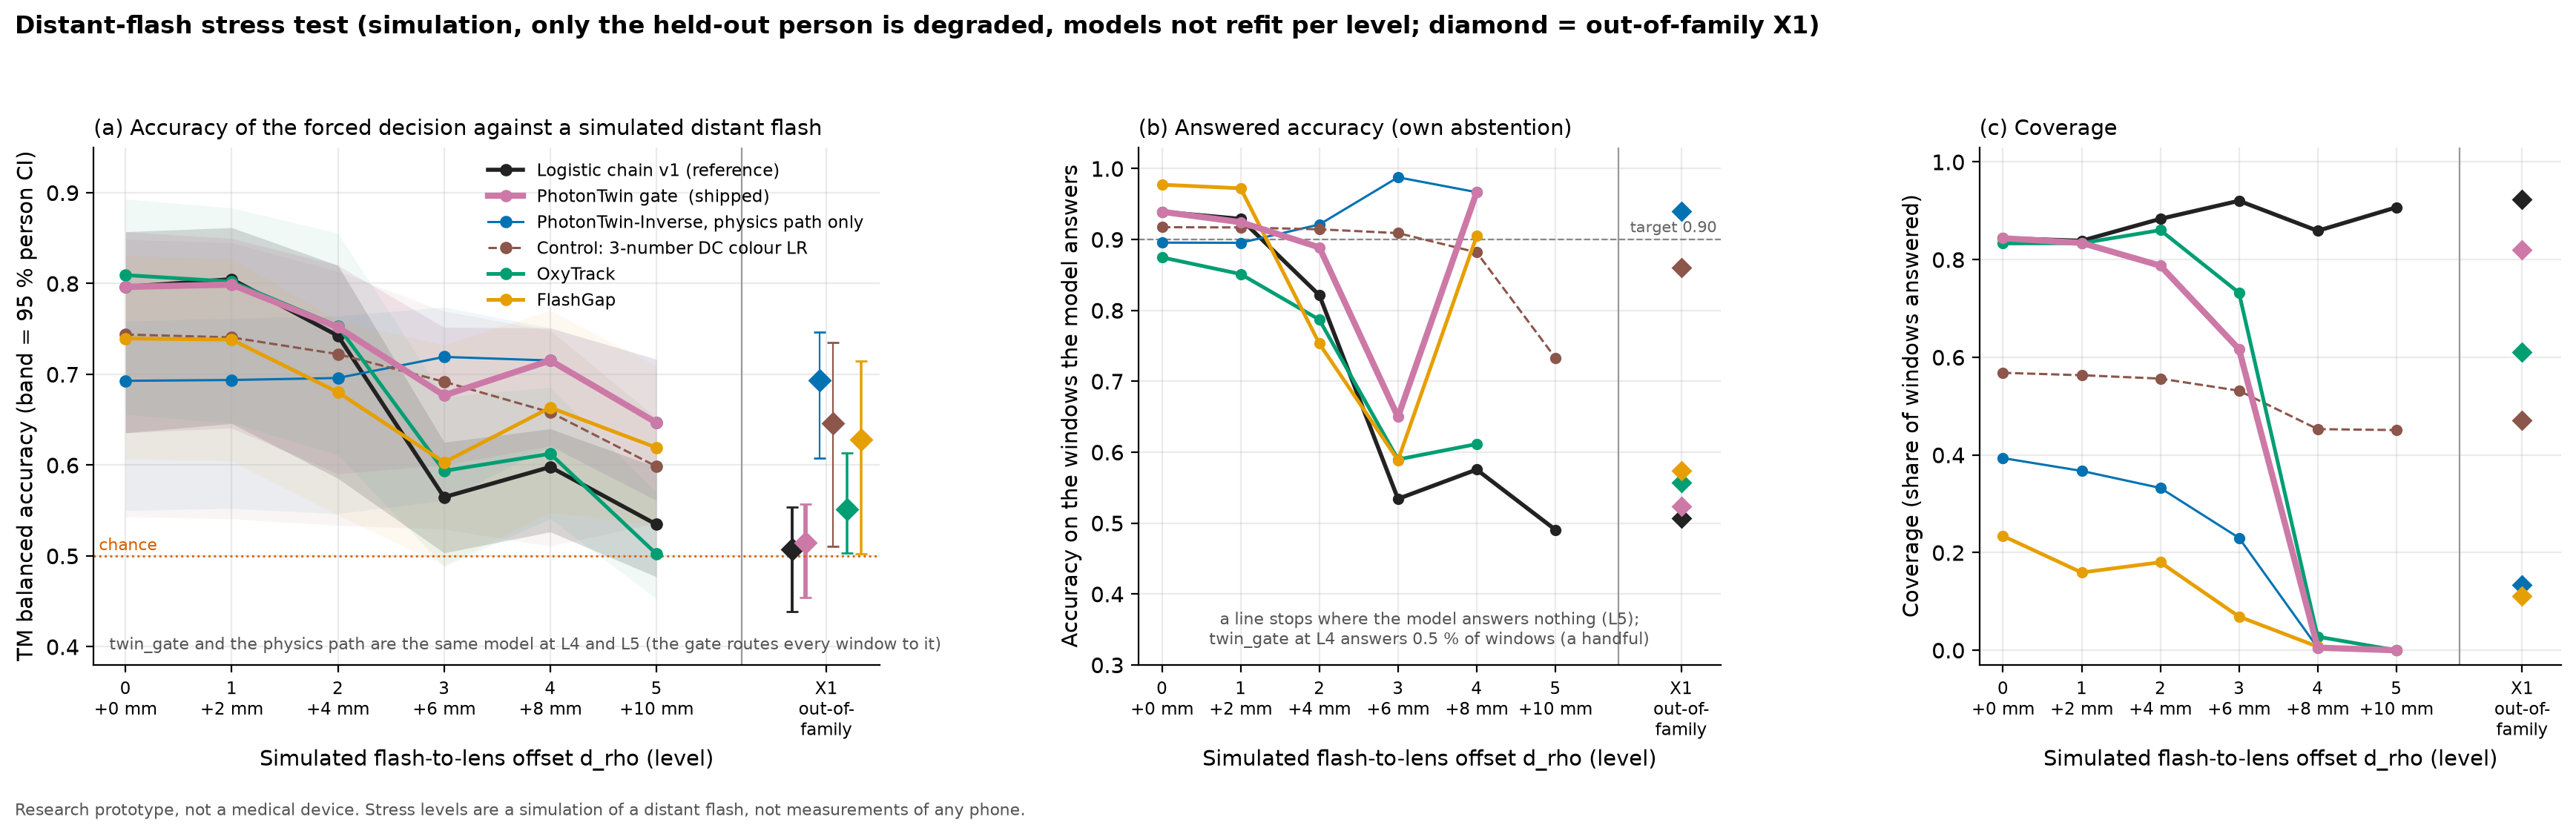
\includegraphics[width=0.94\linewidth]{../docs/figures/photon_stress_curve.png}
\caption{Simulated distant-flash stress, a simulation and not a phone measurement. Only the held-out person is degraded; diamonds are X1. (a) TM of the forced decision, with bands for the chain and the shipped model. (b) Accuracy on answered windows. (c) Coverage. The chain keeps answering at about chance; PhotonDistill2 answers fewer windows and keeps its answered accuracy near 0.9. The colour control (dashed) is nearly as robust.}\label{fig:stresscurve}
\end{figure}

\begin{figure}[tbp]
\centering
\begin{minipage}[b]{0.5\linewidth}\centering
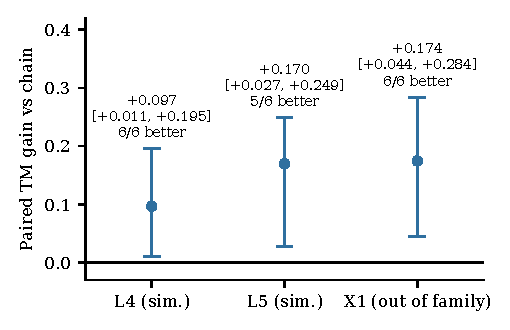
\includegraphics[width=\linewidth]{figures_ieee/fig_stress_gain.pdf}
\end{minipage}\hfill
\begin{minipage}[b]{0.47\linewidth}
\caption{Paired TM gain of PhotonDistill2 over the chain under simulated distant flash, with 95\% person-bootstrap intervals and people better. L4 and L5 are in-simulator; X1 is out of family. Simulation only.}\label{fig:gain}
\end{minipage}
\end{figure}

% =====================================================================
\section{Failure Analysis}\label{sec:failure}
\paragraph{Failure modes} Motion bursts, cold fingers, a weak far-flash signal and a clipped red channel each make the pulse unusable, and the app answers \emph{Unsure} for them (Fig.~\ref{fig:modes}). On real out-of-fold scores the scores lag the onset of desaturation, the main source of missed low windows.

\paragraph{Timeline of the worst person} Fig.~\ref{fig:timeline} follows the chain through two recordings of person 4 and one of person 5 (\code{results/timeline_notes.json}). On person 4's left hand the chain is right on 82.3\% of windows; its 79 false alarms come at reference values of 90.0 to 95.9\%, from 212~s, before the first value below 90 at 372~s. On the right hand accuracy is 72.7\%, with 107 missed low windows between 414 and 874~s and 29.8\% abstained. On person 5's left hand accuracy is 91.6\%, and the 30 false alarms sit at 90.0 to 91.6\%.

\begin{figure}[tbp]
\centering
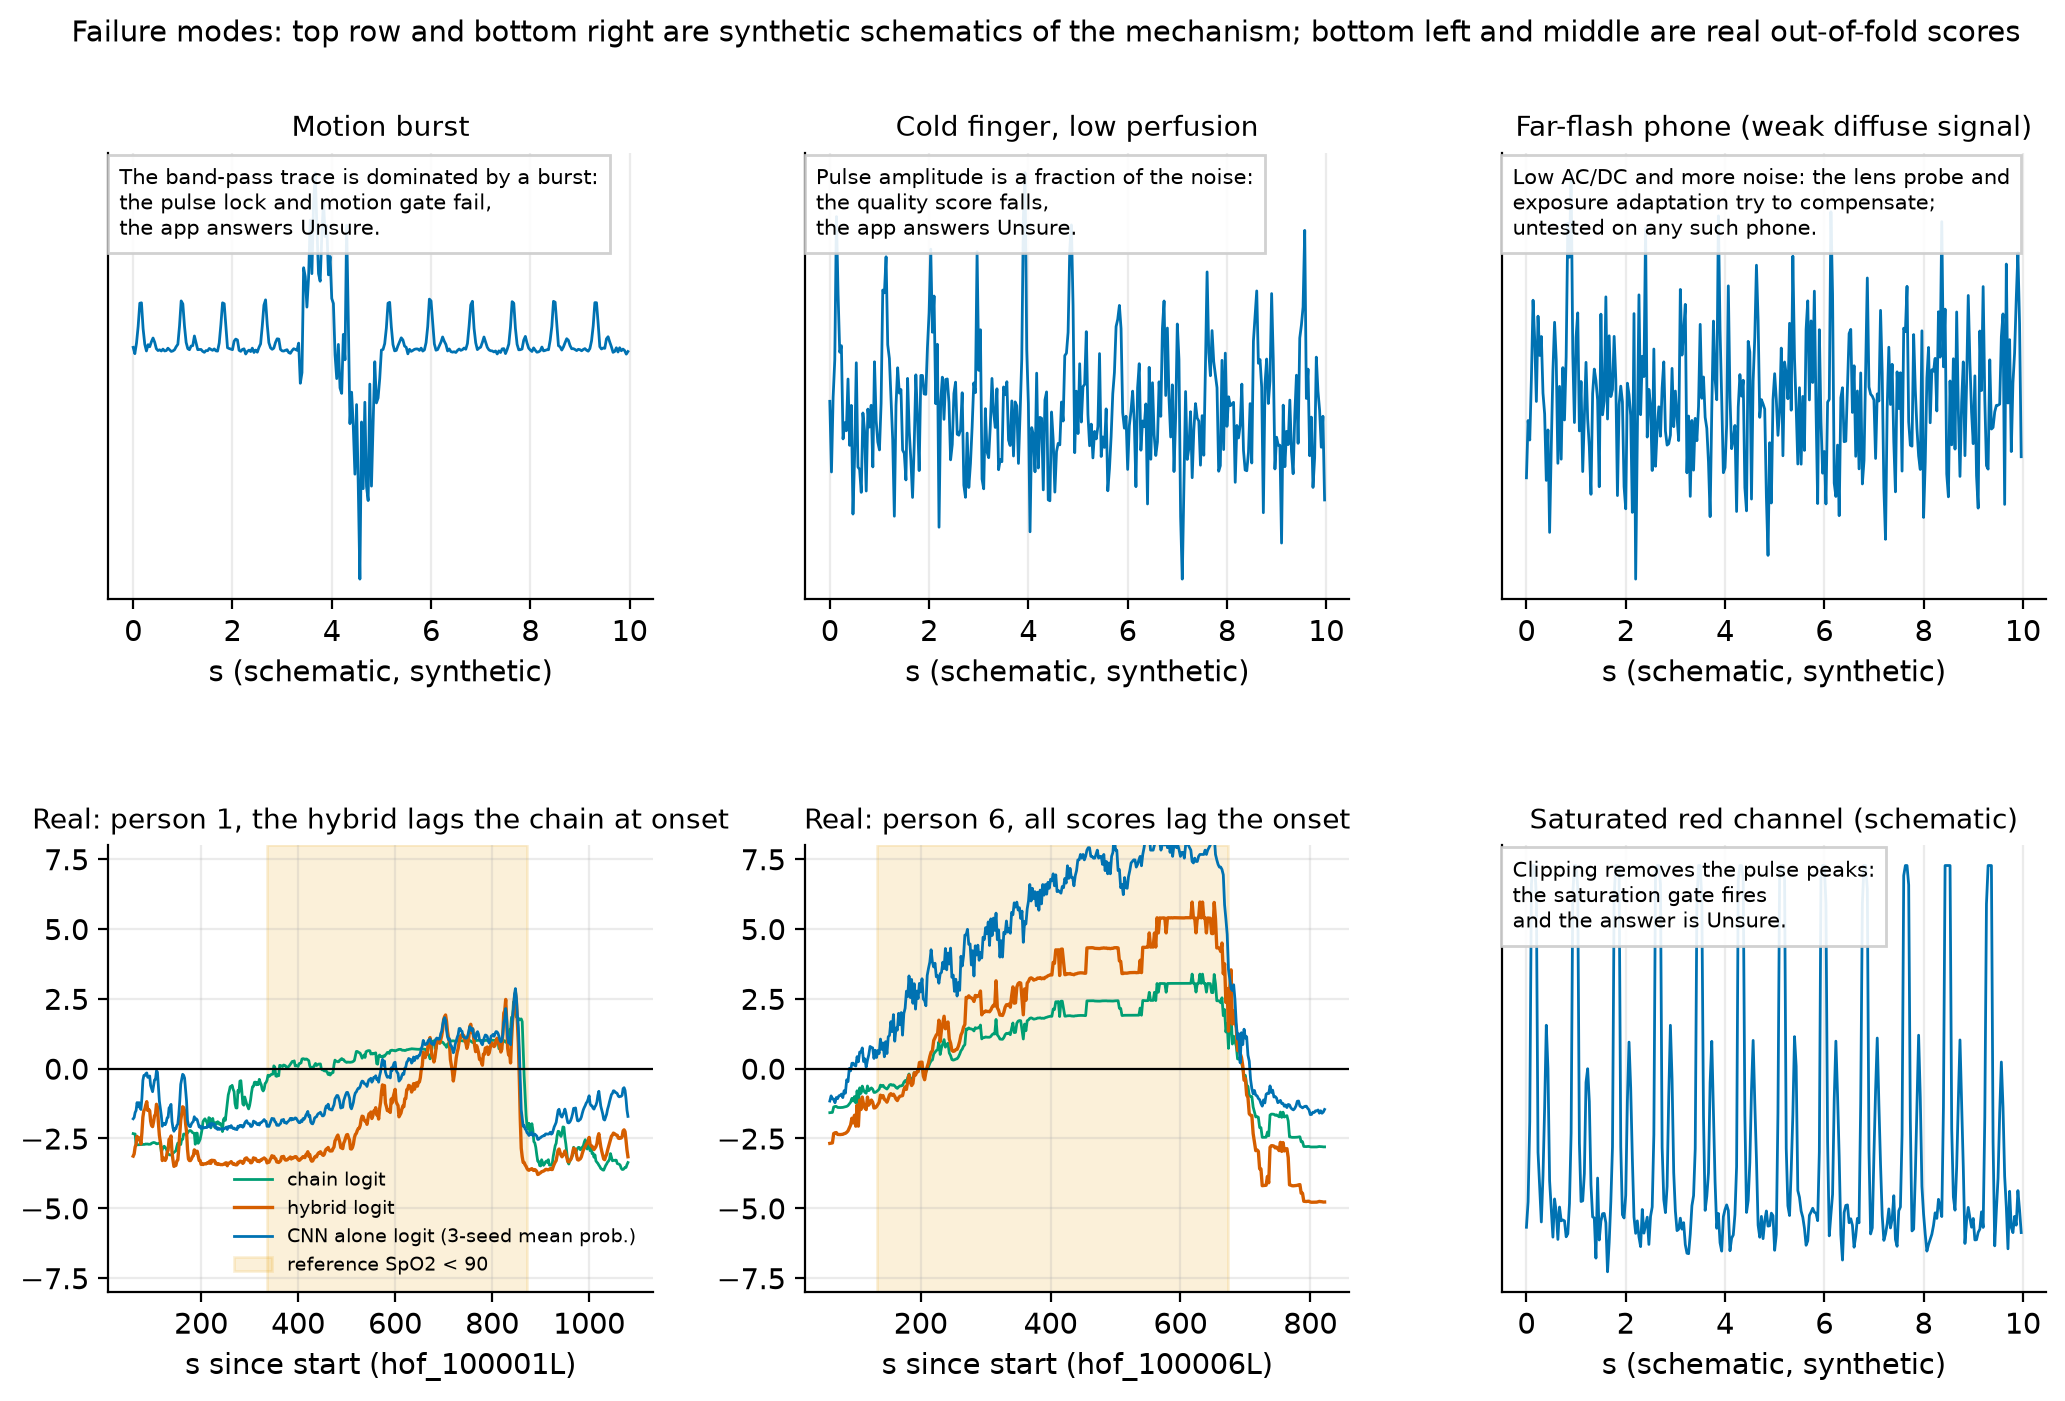
\includegraphics[width=0.54\linewidth]{../docs/figures/ml_failure_modes.png}
\caption{Failure modes. Top row and bottom right: synthetic schematics of the mechanism (motion burst, low perfusion, weak far-flash signal, clipped red channel). Bottom left and middle: real out-of-fold logits of the chain, the earlier hybrid and the CNN on recordings 100001L and 100006L, with the reference \spo{}~$<90$ interval shaded; scores lag the onset.}\label{fig:modes}
\end{figure}

\begin{figure}[tbp]
\centering
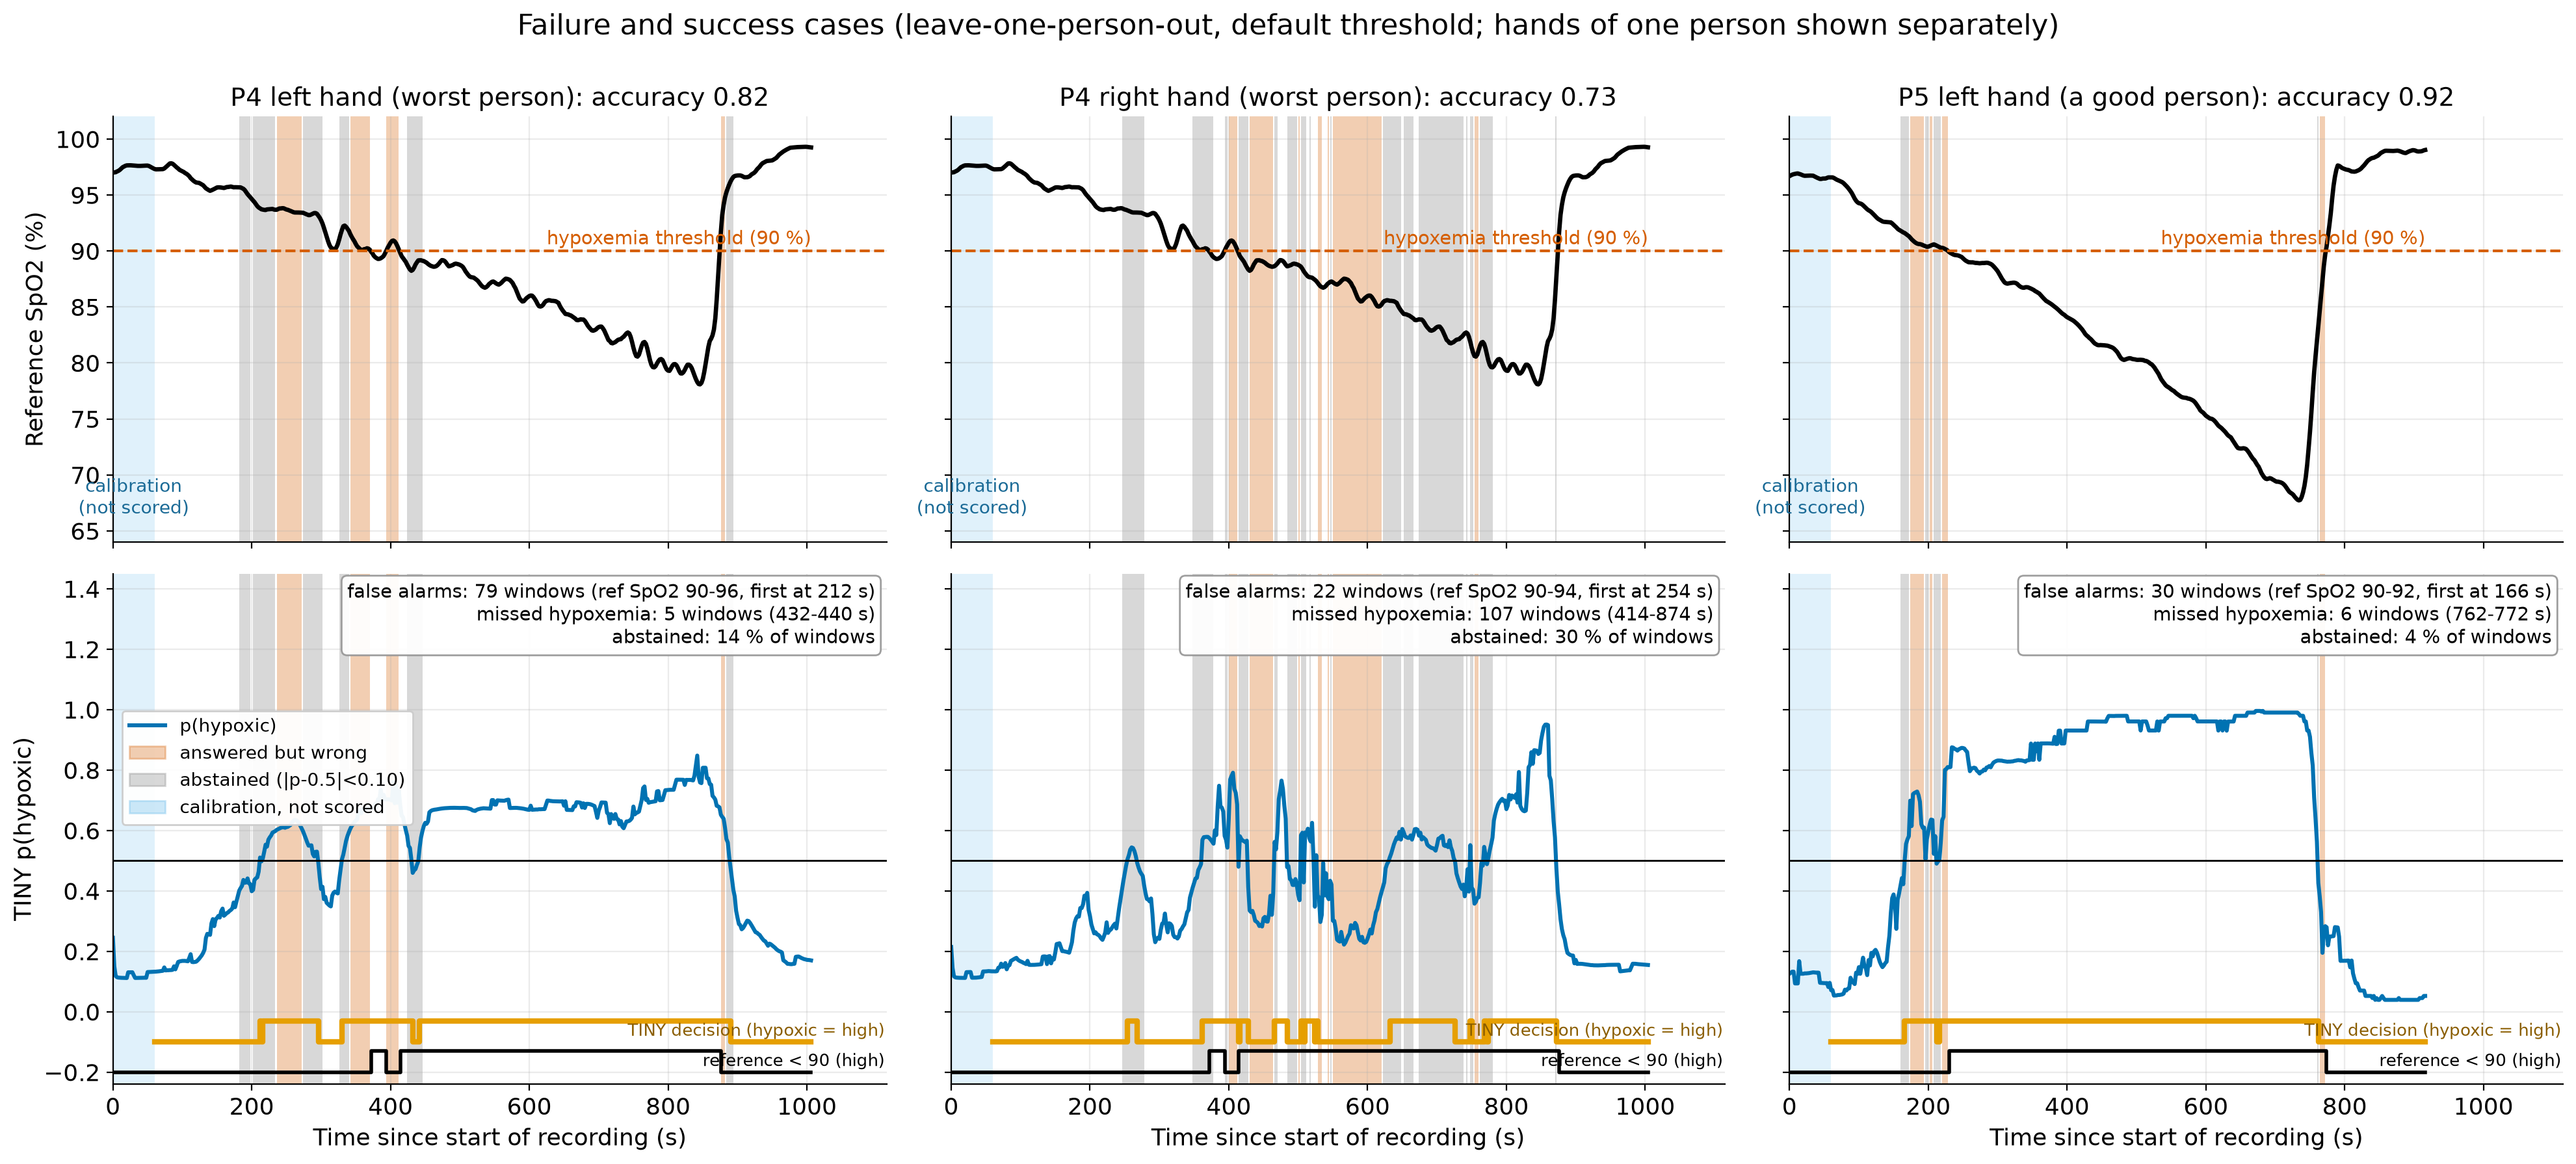
\includegraphics[width=0.88\linewidth]{../docs/figures/fig_timeline_failure.png}
\caption{Failure and success cases of the chain (``TINY''), LOSO at the default threshold, hands shown separately. Top: reference \spo{} and the 90\% line. Bottom: $p(\text{hypoxic})$, decision and reference label. Orange: answered but wrong; grey: abstained ($|p-0.5|<0.10$); blue: calibration minute. Person 4's right hand is missed for most of the desaturation; the left hand's false alarms precede the drop below 90\%.}\label{fig:timeline}
\end{figure}

\paragraph{Exercise false alarms} The heart-rate rise is not oxygen-specific. On the moshekam exercise recordings, with normal \spo{}, the heart-rate rule flags 68.4\% of normoxic windows over the 13 people with an extracted heart rate (63.4\% over all 14), against resting false-positive rates of 14.2\% for the chain and 18.8\% for the heart-rate rise alone on Hoffman (Fig.~\ref{fig:exercise}). The app therefore requires seated rest and a motion gate.

\begin{figure}[tbp]
\centering
\begin{minipage}[b]{0.46\linewidth}\centering
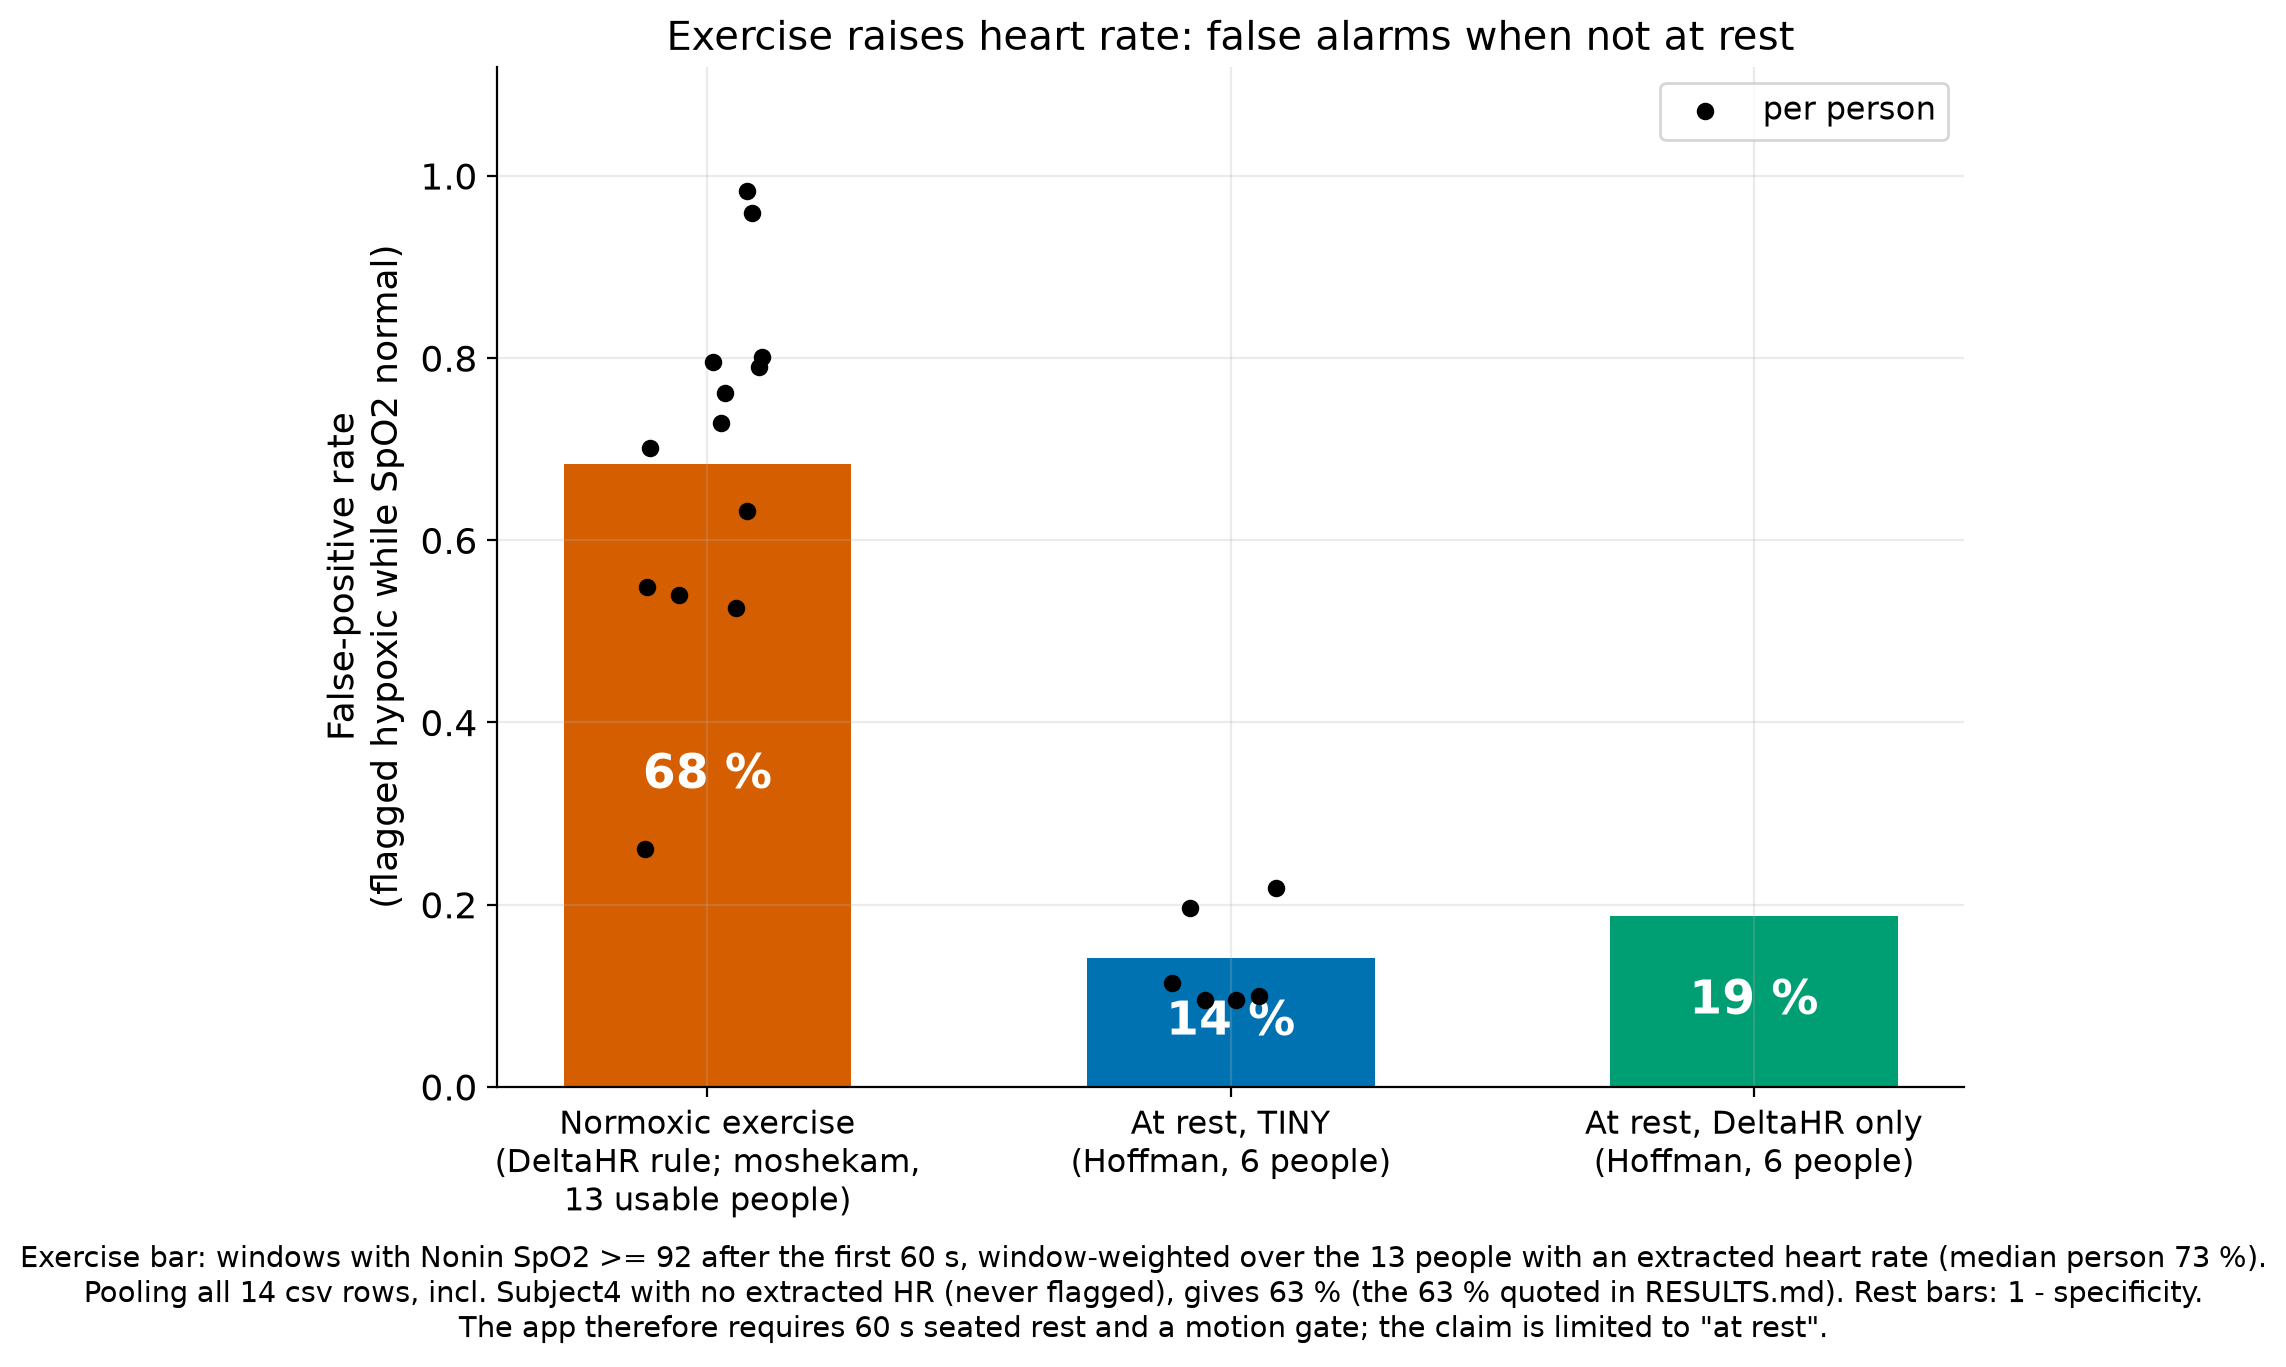
\includegraphics[width=\linewidth]{../docs/figures/fig_exercise_false_alarm.png}
\end{minipage}\hfill
\begin{minipage}[b]{0.51\linewidth}
\caption{Exercise raises heart rate and causes false alarms (\code{results/exercise_vs_rest_fpr.csv}). False-positive rate on normoxic windows for the heart-rate rule during exercise (moshekam, 13 people, dots per person) and for the chain and the heart-rate rise alone at rest (Hoffman, six people). The method is limited to people at rest.}\label{fig:exercise}
\end{minipage}
\end{figure}

\paragraph{Skin tone: the OpenOximetry analysis}\label{sec:skin} The Hoffman set has one dark-skinned participant, so no phone skin-tone claim is possible. On 34 OpenOximetry people held out of every stage (24 with arterial \sao{}, 33,001 windows; label lag 19~s [15, 27] learned on 63 training people), the CNN has an MAE of 2.94 [2.45, 3.50] points against 3.07 [2.60, 3.54] for the textbook rule $110-25R$ (paired $-0.13$ [$-0.47$, $+0.26$], a tie) and 7.38 for the training mean (\code{results/ml/openox_spo2_*.csv}). The dark-minus-light gap by ITA tertile is $+0.41$ [$-0.75$, $+1.63$] (7 against 6 people), a tie; Monk 7+ has 2 held-out people and is suppressed. The reference itself is biased (Fig.~\ref{fig:skin}): over 137 people with draws, the oximeter display minus \sao{} is $+1.77$ [$+0.64$, $+2.61$] points higher for Monk 7+ than Monk 1--3 (7 against 55 people) and $+1.10$ [$+0.65$, $+1.55$] for the darkest against the lightest ITA tertile, in the direction of earlier studies \cite{bickler2005,feiner2007,sjoding2020}. Phone labels come from pulse oximeters and inherit this bias; no phone claim follows from a contact sensor.

\begin{figure}[tbp]
\centering
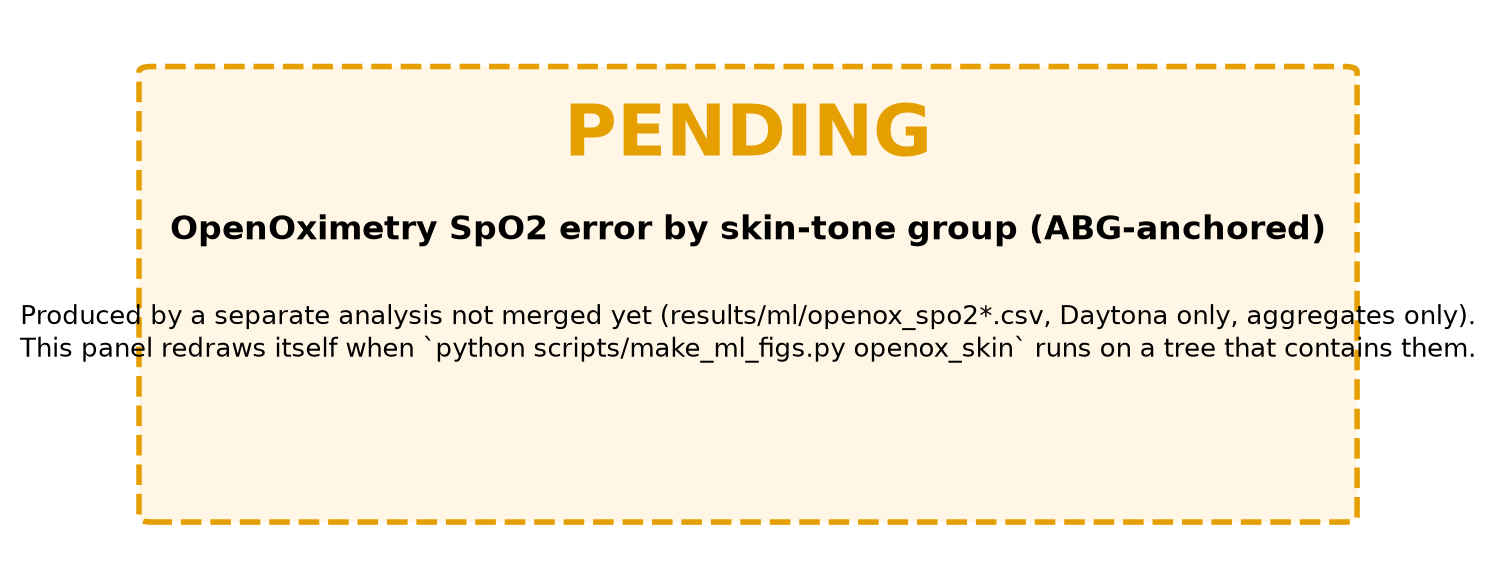
\includegraphics[width=0.66\linewidth]{../docs/figures/ml_openox_skin.png}
\caption{OpenOximetry contact red/infrared sensor with arterial blood gas; not a phone test, aggregates only. Left: \sao{} MAE by skin-tone group for the CNN and the textbook ratio-of-ratios on 24 held-out people; Monk 7+ (2 people) is suppressed. Right: oximeter display minus blood-gas \sao{} over all people with draws; the device over-reads more in darker skin.}\label{fig:skin}
\end{figure}

% =====================================================================
\section{Deployment}\label{sec:deploy}
\paragraph{In-browser runtime} The app is static files with no build step and works offline through a service worker. Every 2~s it computes the 39 features in JavaScript and runs the three students in a small dependency-free MLP runtime, with a median latency of about 15~ms per window in Chromium on a development laptop; phones are slower by an unmeasured factor. The chain stays behind \code{?engine=logistic} and the earlier hybrid behind \code{?engine=hybrid}, whose CNN runs in a Web Worker (16.4~ms per forward pass on the laptop) so that it never delays camera frames.

\paragraph{Parity tests} The results come from the Python code, so the app must compute the same numbers. Tests check the v1 and v2 chains, the heart-rate estimator, the CNN and the PhotonDistill2 engine against Python references on fixture recordings. The app forward pass reproduces the reference scores of the fixture windows to $2.4\times10^{-9}$ with identical answer flags, and the JavaScript and Python MLPs agree to about $10^{-13}$. An ONNX export matches the float64 reference to $1.3\times10^{-7}$ over 1,280 windows. A fake-camera browser test checks a good recording, a refused grey frame, two replays, and stalls that must flip to \emph{Unsure} or reject the calibration (\code{results/photon/EXPORT_CHECK.md}).

\paragraph{Privacy} Video never leaves the phone. Each frame is averaged to three numbers in the browser and discarded; the app stores and uploads nothing, and optional trace downloads go only to the user's own device. The model does not train on user data.

% =====================================================================
\section{Limitations}\label{sec:limits}
The test set has six people, 12 recordings and one phone model, all at rest in a laboratory protocol, with one dark-skinned participant, so we make no phone skin-tone claim. The effective sample is six people, so ``tie'' often means ``cannot distinguish''. All candidates after round 1 were designed after earlier held-out results on the same people had been seen (Amendments 6 to 8); PhotonDistill2's wider grid was chosen because the round-2 distillation weight hit the grid edge in every fold. Rounds 2 and 3 are therefore optimistic on clean light, and picking the round-3 winner by its point estimate adds an unquantified selection effect. PhotonDistill2's null and stress files landed at 20:16 CT, one minute after the 20:15 cutoff of the round-3 rule; the selection script flagged them as late, and the planner locked the model anyway and recorded the waiver.

The stress levels are a simulation with a design-chosen path scale, and L1 to L5 lie inside the augmentation prior. Real devices differ in exposure control, colour processing and flash spectrum, phones with a distant flash are untested, and capture on current iPhones is unreliable in our own use. The label is a pulse-oximeter reading, not arterial blood. The method measures a drop from the person's first minute and cannot tell whether the person was already low. Exercise, arrhythmia and a resting pulse below 51~bpm break the signal. No model in this study beats the chain on clean light.

\section{Ethics and Disclaimer}\label{sec:ethics}
This is a research prototype, not a medical device. It does not measure \spo{} and does not diagnose. ``Normal vs your baseline'' is never reassurance, because the model cannot detect that a person was already low during the baseline minute. A possible-low result is a prompt to re-check with a pulse oximeter or seek care; no one should delay care or replace a pulse oximeter or clinician with this app. It has not been validated on any phone or for any skin tone \cite{bickler2005,feiner2007,sjoding2020}. All human data come from public or credentialed datasets collected by others under their own consent procedures; OpenOximetry and MTHS results are published as aggregates only, and weights trained on their rows are shared for non-commercial research and education only.

\section{Conclusion and Future Work}\label{sec:conclusion}
On six people, a distilled network for phone-camera hypoxemia screening is on par with a logistic chain of hand-built features on clean light (\WinLzero{} against \ChainLzero{}, paired \WinLzeroDiff{} \WinLzeroDiffCI{}) and does not beat it. Under a simulated distant flash it keeps more accuracy than the chain (paired \WinXoneDiff{} \WinXoneDiffCI{} at the out-of-family level X1) and abstains more as the light weakens, but a three-number colour control explains most of that gain. We expect the harness to be the most reusable part. Next steps: record real phones with distant flashes to check the simulation against measurements; record more people across skin tones with arterial references; pre-register the next candidate and its rule before any score on new people and test it once; and add an independently established baseline so that a person already low at the start can be detected.

\section*{Acknowledgments}
We thank the authors of the Hoffman, MTHS, BUT PPG, OpenOximetry, PTT-PPG and BIDMC datasets, the maintainers of PhysioNet, and the authors of the published optical constants used by PhotonTwin.

{\footnotesize
\setstretch{1.0}
\bibliographystyle{IEEEtran}
\bibliography{oxydrop_ieee_refs}
}

\end{document}
